% This is the Reed College LaTeX thesis template. Most of the work
% for the document class was done by Sam Noble (SN), as well as this
% template. Later comments etc. by Ben Salzberg (BTS). Additional
% restructuring and APA support by Jess Youngberg (JY).
% Your comments and suggestions are more than welcome; please email
% them to cus@reed.edu
%
% See http://web.reed.edu/cis/help/latex.html for help. There are a
% great bunch of help pages there, with notes on
% getting started, bibtex, etc. Go there and read it if you're not
% already familiar with LaTeX.
%
% Any line that starts with a percent symbol is a comment.
% They won't show up in the document, and are useful for notes
% to yourself and explaining commands.
% Commenting also removes a line from the document;
% very handy for troubleshooting problems. -BTS

% As far as I know, this follows the requirements laid out in
% the 2002-2003 Senior Handbook. Ask a librarian to check the
% document before binding. -SN

%%
%% Preamble
%%
% \documentclass{<something>} must begin each LaTeX document
\documentclass[12pt,twoside,openany]{reedthesis}
% Packages are extensions to the basic LaTeX functions. Whatever you
% want to typeset, there is probably a package out there for it.
% Chemistry (chemtex), screenplays, you name it.
% Check out CTAN to see: http://www.ctan.org/
%%

\usepackage{setspace}
\usepackage{graphicx,latexsym}
\usepackage{amsmath}
\usepackage{amssymb,amsthm}
%\usepackage{longtable,booktabs,setspace}
\usepackage{longtable,booktabs,setspace, array}
\usepackage{chemarr} %% Useful for one reaction arrow, useless if you're not a chem major
\usepackage[hyphens]{url}
% Added by CII
\usepackage{hyperref}
\usepackage{lmodern}
\usepackage{float}
\floatplacement{figure}{H}
% End of CII addition
\usepackage{rotating}
% Next line commented out by CII
%%% \usepackage{natbib}
% Comment out the natbib line above and uncomment the following two lines to use the new
% biblatex-chicago style, for Chicago A. Also make some changes at the end where the
% bibliography is included.
%\usepackage{biblatex-chicago}
%\bibliography{thesis}


% Added by CII (Thanks, Hadley!)
% Use ref for internal links
\renewcommand{\hyperref}[2][???]{\autoref{#1}}
\def\chapterautorefname{Chapter}
\def\sectionautorefname{Section}
\def\subsectionautorefname{Subsection}
% End of CII addition

% Added by CII
\usepackage{caption}
\captionsetup{width=5in}
% End of CII addition

% \usepackage{times} % other fonts are available like times, bookman, charter, palatino

% Syntax highlighting #22
  \usepackage{color}
  \usepackage{fancyvrb}
  \newcommand{\VerbBar}{|}
  \newcommand{\VERB}{\Verb[commandchars=\\\{\}]}
  \DefineVerbatimEnvironment{Highlighting}{Verbatim}{commandchars=\\\{\}}
  % Add ',fontsize=\small' for more characters per line
  \usepackage{framed}
  \definecolor{shadecolor}{RGB}{248,248,248}
  \newenvironment{Shaded}{\begin{snugshade}}{\end{snugshade}}
  \newcommand{\AlertTok}[1]{\textcolor[rgb]{0.94,0.16,0.16}{#1}}
  \newcommand{\AnnotationTok}[1]{\textcolor[rgb]{0.56,0.35,0.01}{\textbf{\textit{#1}}}}
  \newcommand{\AttributeTok}[1]{\textcolor[rgb]{0.77,0.63,0.00}{#1}}
  \newcommand{\BaseNTok}[1]{\textcolor[rgb]{0.00,0.00,0.81}{#1}}
  \newcommand{\BuiltInTok}[1]{#1}
  \newcommand{\CharTok}[1]{\textcolor[rgb]{0.31,0.60,0.02}{#1}}
  \newcommand{\CommentTok}[1]{\textcolor[rgb]{0.56,0.35,0.01}{\textit{#1}}}
  \newcommand{\CommentVarTok}[1]{\textcolor[rgb]{0.56,0.35,0.01}{\textbf{\textit{#1}}}}
  \newcommand{\ConstantTok}[1]{\textcolor[rgb]{0.00,0.00,0.00}{#1}}
  \newcommand{\ControlFlowTok}[1]{\textcolor[rgb]{0.13,0.29,0.53}{\textbf{#1}}}
  \newcommand{\DataTypeTok}[1]{\textcolor[rgb]{0.13,0.29,0.53}{#1}}
  \newcommand{\DecValTok}[1]{\textcolor[rgb]{0.00,0.00,0.81}{#1}}
  \newcommand{\DocumentationTok}[1]{\textcolor[rgb]{0.56,0.35,0.01}{\textbf{\textit{#1}}}}
  \newcommand{\ErrorTok}[1]{\textcolor[rgb]{0.64,0.00,0.00}{\textbf{#1}}}
  \newcommand{\ExtensionTok}[1]{#1}
  \newcommand{\FloatTok}[1]{\textcolor[rgb]{0.00,0.00,0.81}{#1}}
  \newcommand{\FunctionTok}[1]{\textcolor[rgb]{0.00,0.00,0.00}{#1}}
  \newcommand{\ImportTok}[1]{#1}
  \newcommand{\InformationTok}[1]{\textcolor[rgb]{0.56,0.35,0.01}{\textbf{\textit{#1}}}}
  \newcommand{\KeywordTok}[1]{\textcolor[rgb]{0.13,0.29,0.53}{\textbf{#1}}}
  \newcommand{\NormalTok}[1]{#1}
  \newcommand{\OperatorTok}[1]{\textcolor[rgb]{0.81,0.36,0.00}{\textbf{#1}}}
  \newcommand{\OtherTok}[1]{\textcolor[rgb]{0.56,0.35,0.01}{#1}}
  \newcommand{\PreprocessorTok}[1]{\textcolor[rgb]{0.56,0.35,0.01}{\textit{#1}}}
  \newcommand{\RegionMarkerTok}[1]{#1}
  \newcommand{\SpecialCharTok}[1]{\textcolor[rgb]{0.00,0.00,0.00}{#1}}
  \newcommand{\SpecialStringTok}[1]{\textcolor[rgb]{0.31,0.60,0.02}{#1}}
  \newcommand{\StringTok}[1]{\textcolor[rgb]{0.31,0.60,0.02}{#1}}
  \newcommand{\VariableTok}[1]{\textcolor[rgb]{0.00,0.00,0.00}{#1}}
  \newcommand{\VerbatimStringTok}[1]{\textcolor[rgb]{0.31,0.60,0.02}{#1}}
  \newcommand{\WarningTok}[1]{\textcolor[rgb]{0.56,0.35,0.01}{\textbf{\textit{#1}}}}

% To pass between YAML and LaTeX the dollar signs are added by CII
\title{Regime Detection Measures for the Practical Ecologist}
\author{Jessica L. Burnett}
% The month and year that you submit your FINAL draft TO THE LIBRARY
\date{2019}
% \division{}
\advisor{Craig R. Allen}
\department{School of Natural Resources}
\institution{University of Nebraska-Lincoln}
\degree{Doctor of Philosophy}
%If you have two advisors for some reason, you can use the following
% Uncommented out by CII
\altadvisor{Dirac Twidwell}
% End of CII addition

%%% Remember to use the correct department!
% if you're writing a thesis in an interdisciplinary major,
% uncomment the line below and change the text as appropriate.
% check the Senior Handbook if unsure.
%\thedivisionof{The Established Interdisciplinary Committee for}
% if you want the approval page to say "Approved for the Committee",
% uncomment the next line
%\approvedforthe{Committee}

% Added by CII
%%% Copied from knitr
%% maxwidth is the original width if it's less than linewidth
%% otherwise use linewidth (to make sure the graphics do not exceed the margin)
\makeatletter
\def\maxwidth{ %
  \ifdim\Gin@nat@width>\linewidth
    \linewidth
  \else
    \Gin@nat@width
  \fi
}
\makeatother

\renewcommand{\contentsname}{Table of Contents}
% End of CII addition

\setlength{\parskip}{0pt}

% Added by CII

\providecommand{\tightlist}{%
  \setlength{\itemsep}{0pt}\setlength{\parskip}{0pt}}

\Acknowledgements{
Graduate school itself isn't hard, but the journey is. I have a lot of people and institutions to thank for their emotional, intellectual, financial, and other support. I wish to first highlight how \textbf{great it was to be a graduate student at this university and in the School of Natural Resources}. UNL has provided tremendous support at all levels of the university. Although I am not a fan of Nebraska's climate, I highly recommend this school to prospective students.
I thank my supervisors, Craig Allen and Dirac Twidwell, for providing me with this amazing opportunity and for supporting my growth as an independent researcherm and my committee members, Craig Allen, David Angeler, John De Long, Dirac Twidwell, and Drew Tyre for their support and advisement, but especially for their comprehensive examination--I found this process transformative, albeit very stress inducing. I also wish to thank Dirac for his comprehensive exam questions--I never knew how much I didn't know until I studied your recommendations. I also thank Craig for supporting my efforts to study and conduct research outside of our immediate geographical settings. Studying at the International Institute for Applied Systems Analysis was an amazing opportunity! I thank Brian Fath and Elena Rovenskaya for their advisement, members of the Applied Systems Analysis research group for their feedback on my research, and to the postdocs and YSSPers.
I would like to especially thank some of the amazing and brilliant \textbf{female scientists} in my life for their encouragement: Jane Anderson, Karen Bailey, Hannah Birge, Mary Bomberger Brown, Tori Donovan, Brittany Dueker, Allie Schiltmeyer, Katie Sieving, Erica Stuber, Becky Wilcox, Carissa Wonkka, and Lyndsie Wszola. I thank these women and others for their contributions to my professional development: David Angeler, Christie Bahlai, Mary Bomberger Brown, John Carroll, Jenny Dauer, John DeLong, Tarsha Eason, Brian Fath, Ahjond Garmestani, Chris Lepczyk, Frank La Sorte, Chai Molina, Zac Warren, Hao Ye and Peter Zebrowski. I owe thanks to Craig Allen and Kevin Pope for entertaining my many hours of discussion (interrogation?) regarding federal employment. I also thank fellow graduate students whom I hope I have forged strong and lasting connections: Hannah Birge, Tori Donovan, Caleb Roberts, Allie Schiltmeyer, and Lyndsie Wszola
I am one of the many graduate students afflicted with mental health ``disorders''. I am first grafteful to one friend (H) who unknowingly destigmatized mental health in my mind and wihtout whom I may not have sought treatment. I applaud students and faculty who have been outspoken regarding mental health related issues, and I am indebtted to my general practitioner and mental health advocate, Terry Thomas M.A., M.S.N., A.P.R.N.\\
\emph{Financial support}. This research was funded by the U.S. Department of Defense's Strategic Environmental Research and Development Program (project ID: RC-2510). The University of Nebraska-Lincoln (UNL) has been highy supportive in my doctoral studies and reserach. I am grateful for the generous of donors to the University of Nebraska Foundation, which provided me with two prestigious supplemental fellowships: Fling and Othmer. I also thank the Nelson Family (Nelson Memorial Fellowship) and the Institute of Agriculture and Natural Resources, who funded large portions of my academic and research-related travel. I thank the School of Natural Resources for their financial support in my conference travel. The U.S. National Academy of Sciences generously funded part of my travel to the International Institute for Applied Systems Analysis (IIASA). This financial support provided me not only with invaluabe opportunities to attend and present at national and international conferences and workshops, conduct research abroad, and network--this funding alleviated some financial pressures associated with graduate school which allowed a more refined focus on my dissertation research. The opportunities and experiences provided to me by each funding source were amazing, thank you.
Finally, to my partner of eight years--Schultzie--thank you for everything. Just kidding, thank you, Nat Price, you are amazing.
}

\Dedication{
To the end-users and researchers frustrated with jargon and lack of practical utility of ecological models and metrics. And to Mike Moulton, without whose support and encouragement many years ago two advanced degrees would likely not have been possible.
}

\Preface{

}

\Abstract{

}

% End of CII addition
%%
%% End Preamble
%%
%
\begin{document}

% Everything below added by CII
  \maketitle

\frontmatter % this stuff will be roman-numbered
\pagestyle{empty} % this removes page numbers from the frontmatter
  \begin{acknowledgements}
    Graduate school itself isn't hard, but the journey is. I have a lot of people and institutions to thank for their emotional, intellectual, financial, and other support. I wish to first highlight how \textbf{great it was to be a graduate student at this university and in the School of Natural Resources}. UNL has provided tremendous support at all levels of the university. Although I am not a fan of Nebraska's climate, I highly recommend this school to prospective students.
    I thank my supervisors, Craig Allen and Dirac Twidwell, for providing me with this amazing opportunity and for supporting my growth as an independent researcherm and my committee members, Craig Allen, David Angeler, John De Long, Dirac Twidwell, and Drew Tyre for their support and advisement, but especially for their comprehensive examination--I found this process transformative, albeit very stress inducing. I also wish to thank Dirac for his comprehensive exam questions--I never knew how much I didn't know until I studied your recommendations. I also thank Craig for supporting my efforts to study and conduct research outside of our immediate geographical settings. Studying at the International Institute for Applied Systems Analysis was an amazing opportunity! I thank Brian Fath and Elena Rovenskaya for their advisement, members of the Applied Systems Analysis research group for their feedback on my research, and to the postdocs and YSSPers.
    I would like to especially thank some of the amazing and brilliant \textbf{female scientists} in my life for their encouragement: Jane Anderson, Karen Bailey, Hannah Birge, Mary Bomberger Brown, Tori Donovan, Brittany Dueker, Allie Schiltmeyer, Katie Sieving, Erica Stuber, Becky Wilcox, Carissa Wonkka, and Lyndsie Wszola. I thank these women and others for their contributions to my professional development: David Angeler, Christie Bahlai, Mary Bomberger Brown, John Carroll, Jenny Dauer, John DeLong, Tarsha Eason, Brian Fath, Ahjond Garmestani, Chris Lepczyk, Frank La Sorte, Chai Molina, Zac Warren, Hao Ye and Peter Zebrowski. I owe thanks to Craig Allen and Kevin Pope for entertaining my many hours of discussion (interrogation?) regarding federal employment. I also thank fellow graduate students whom I hope I have forged strong and lasting connections: Hannah Birge, Tori Donovan, Caleb Roberts, Allie Schiltmeyer, and Lyndsie Wszola
    I am one of the many graduate students afflicted with mental health ``disorders''. I am first grafteful to one friend (H) who unknowingly destigmatized mental health in my mind and wihtout whom I may not have sought treatment. I applaud students and faculty who have been outspoken regarding mental health related issues, and I am indebtted to my general practitioner and mental health advocate, Terry Thomas M.A., M.S.N., A.P.R.N.\\
    \emph{Financial support}. This research was funded by the U.S. Department of Defense's Strategic Environmental Research and Development Program (project ID: RC-2510). The University of Nebraska-Lincoln (UNL) has been highy supportive in my doctoral studies and reserach. I am grateful for the generous of donors to the University of Nebraska Foundation, which provided me with two prestigious supplemental fellowships: Fling and Othmer. I also thank the Nelson Family (Nelson Memorial Fellowship) and the Institute of Agriculture and Natural Resources, who funded large portions of my academic and research-related travel. I thank the School of Natural Resources for their financial support in my conference travel. The U.S. National Academy of Sciences generously funded part of my travel to the International Institute for Applied Systems Analysis (IIASA). This financial support provided me not only with invaluabe opportunities to attend and present at national and international conferences and workshops, conduct research abroad, and network--this funding alleviated some financial pressures associated with graduate school which allowed a more refined focus on my dissertation research. The opportunities and experiences provided to me by each funding source were amazing, thank you.
    Finally, to my partner of eight years--Schultzie--thank you for everything. Just kidding, thank you, Nat Price, you are amazing.
  \end{acknowledgements}

  \hypersetup{linkcolor=black}
  \setcounter{tocdepth}{2}
  \tableofcontents

  \listoftables

  \listoffigures

  \begin{dedication}
    To the end-users and researchers frustrated with jargon and lack of practical utility of ecological models and metrics. And to Mike Moulton, without whose support and encouragement many years ago two advanced degrees would likely not have been possible.
  \end{dedication}
\mainmatter % here the regular arabic numbering starts
\pagestyle{fancyplain} % turns page numbering back on
% \doublespacing{} % Trying to set spacing between lines in body
\linespread{1} % Trying to set spacing between lines in body

\hypertarget{abstract}{%
\chapter*{Abstract}\label{abstract}}
\addcontentsline{toc}{chapter}{Abstract}

Identifying abrupt changes in the structure and functioning of systems, or system regime shifts, in ecological and social-ecological systems leads to an understanding of relative and absolute system resilience. Resilience is an emergent phenomenon of complex social-ecological systems, and is the ability of a system to absorb disturbance without reorganizing into a new state, or regime. Resilience science provides a framework and methodology for quantitatively assessing the capacity of a system to maintain its current trajectory (or to stay within a certain, and often desirable regime). If and when a system's resilience is exceeded, it crosses a threshold and enters into an alternate regime (or undergoes a regime shift).\\
I will use Fisher Information to detect regime shifts in time and space using avian community data obtained from the North American Breeding Bird Survey within the area east of the Rockies and west of the Mississippi River. Fisher Information is a technique that captures the dynamic of a system, and this metric will be calculated about a suite of bird species abundances aggregated to the route level for all possible time periods. Transmutation (aggregation error) about inclusion or exclusion of certain bird species, functional groups, and guilds will be analyzed. Efforts have been made to develop early warning indicators of regime shifts in ecosystems, however, for most ecosystems there is great uncertainty in predicting the risk of a regime shift, regarding both when and how long it will take to happen and if it can be recognized early enough to be avoided when desired. We will complement the use of Fisher Information with multiple discontinuity analyses about body mass distributions at the route-level to achieve the aim of identifying individual species that best serve as early-warning indicators of regime shifts. For those species found on the edges of body mass aggregations, we test the hypothesis that the background variance in their abundances (on Breeding Bird Survey routes) will increase more than those not observed at the edge of discontinuity aggregations. Identification of early-warning indicators of regime shifts in ecological systems allows management efforts to focus on a single or a small number of species that inform us about ecosystem resilience and trajectory.\\
These methods transcend the primary objective of the Breeding Bird Survey (to monitor population trends) and use this expansive dataset in such a way that information about ecosystem order, trajectory, and resilience emerge. Here, we utilize an expansive dataset (the Breeding Bird Survey) to make broad-scale estimations and predictions about ecosystem resilience, regime status and trajectory, and ecosystem sustainability. Identification of regime shifts and early-warning indicator species may afford us the ability to predict system regime shifts in time.

\hypertarget{intro}{%
\chapter{Introduction}\label{intro}}

Anthropogenic activity in the last few decades will continue to influence the interations within and among ecological systems worldwide. The complexity of and drivers of changes in coupled human-natural systems is consequently altered, further limiting our ability to detect and predict change and impacts of change (Liu et al., 2007; Scheffer, 2009). Early warning systems are developed to detect, and in some cases predict, abrupt changes in disparate systems {[}e.g.~cyber security {[}@{]}, infrastructure {[}@{]}, banking crises (Davis \& Karim, 2008), and agricultural systems{]}. The need to develop and improve early warning systems for natural and coupled human-natural systems is exacerbated by the consequences of climate change and globalization, especially when the human-related stakes are high.

Forecasting undesirable change is, arguably, the holy grail of ecology. Paired with an understanding of system interactions, a forecast isideal if it provides information with sufficient time to prevent or mitigate unwanted systemic change. Early warning systems (or early warning signals, or early warning indicators) have been developed and tested for some ecological systems data (especially marine fisheries time series and for nutrient loading in shallow lakes). Despite the quantitative methods proposed as early warning systems for ecological data (hereafter referred to as regime detection measures, RDMs), most are currently of limited practical utility. This paradox may be a consequence of existing ecological early warning systems (or other quantitative methods for identifying systemic change) having one or more of the following characteristics:
\begin{enumerate}
\def\labelenumi{\arabic{enumi}.}
\tightlist
\item
  not generalizable across systems or system types (especially when it requires a model or a determinsitic function to describe the system)
\item
  require a large number of observations
\item
  difficult to implement
\item
  difficult or to interpret
\item
  requires an understanding of the drivers of change
\item
  performs poorly under uncertainty
\item
  give no uncertaintiy around estimates (tying into interpretation issues)
\item
  cannot handle noisy data
\item
  ignores or does not sufficiently account for observation error
\item
  no baseline with which to compare results
\item
  no application/testing on empirical systems data
\item
  systems are subjectively bounded (i.e., components are chosen)
\item
  being overshadowed by semantics
\item
  are based on two observations (e.g., before-and-after)
\item
  cannot link the shift to potential drivers (i.e.~the method reduces the dimensionality such that it is unitless and/or loses all relevant information)
\end{enumerate}
Research focusing on the above areas as they relate to RDMs will contribute to the advancement and improvement of existing early warning systems, and will, hopefully, highlight methods which are useful and which are not to practitioners and decision makers.

The overarching aim of this dissertation is to advance our understanding of the utility and limitations of select early warning systems. Specifically, I focus on RDMs capable of analyzing multi-varaible data, including temporally- and spatially-explicit. Although the most widely-applied RDMs proposed in the ecological literature are those deveoped for and tested on single-variable time series (e.g., temperature or fisheries stock time series), the utility of these methods in multi-variable systems (data) is limited. Regime detection metrics for tracking and identifying changes in multivariable systems data are of greater use than single-variable RDMs in systems within which a change manifests dynamically and across multiple variables (e.g., species). Multivariable RDMs may also prove advantageous when the drivers of systemic change are unknown. Further, ecological systems are noisy, and ecological systems data are messy.

Although it's taken us many decades to produce realiable weather forecasts 5 days out (and climate is a low-number system..), ecologists produce regime detection methods with the promise of predicting high-dimensional ecosystem change in advance. Many of these RDMs are not models, like the weather forecasting models which have taken years to refine.

\hypertarget{dissertation-structure}{%
\subsection{Dissertation structure}\label{dissertation-structure}}

The chapters hereain are written as separate, publishable manuscripts. Where applicable, co-authors are listed in the front matter of the chapter. The dissertation comprises an introduction to the dissertation (Chapter \ref{intro}), a brief overview of early warning systems (or regime detection measures) for ecological systems data (Chapter \ref{rdmReview}), a detailed guide to Fisher Information as a RDM written for ecologists (Chapter \ref{fiGuide}), an application of Fisher Information to spatially-explicit data (Chapter \ref{fisherSpatial}), introduction of `new' RDM, Distance Travelled (Chapter \ref{distanceTravelled}), a study of data quality and data loss on select RDMs including Distance Travelled and Fisher Information (Chapter \ref{resampling}), and conclusions (Chapter \ref{conclusions}).

\hypertarget{glossary}{%
\section{Glossary}\label{glossary}}

Research surrounding regime shifts, threshold identification, change-point detection, bifurcation theory, etc. is muddled with jargon. Here, I provide a glossary (Table \ref{glossary}) for terms and concepts that may either be unfamiliar to the practical ecologist, or may have multiple meanings among and within ecological researchers and practitioners.

\hypertarget{rdmReview}{%
\chapter{A brief overview of ecological regime detection methods methods}\label{rdmReview}}

\hypertarget{introduction}{%
\section{Introduction}\label{introduction}}
\begin{quote}
\emph{If a regime shift occurs and no one detects it--is it a regime shift at all?}
\end{quote}
\begin{itemize}
\tightlist
\item
  \textbf{No} when a regime shift is defined as a change in a system which negatively impacts humans.
\item
  \textbf{Yes} when a regime shift is defined simply as a shift in the underlying strucutre of a system.
\end{itemize}
Long-lasting changes in the underlying structure or functioning of natural systems due to exogeneous forcings (also called regime shifts) is of interest to ecologists. The ability to identify and predict these shifts is particularly useful for systems which are actively managed, provide ecosystem services, or provide benefit to societiy. There exists a disparity among the number of methods proposed for detecting abrupt changes in ecological, oceanographic, and climatological systems and the studies evaluating these methods using empircal data. Despite the already large number of existing methods and models, new methods continue to permeate the literature. Although reviews of regime shift detection methods exist (Mac Nally, Albano, \& Fleishman, 2014, pp. @scheffer2015generic, @rodionov\_brief\_2005, @roberts2018early, @dakos2015resilience, @mantua\_methods\_2004, @litzow\_early\_2016, @kefi2014early, @andersen\_ecological\_2009, @boettiger\_early\_2013, @dakos\_resilience\_2015, @clements2018indicators, @filatova2016regime, @deyoung\_regime\_2008), the most comprehensive presentation of available methods as they is outdated (S. N. Rodionov, 2005)*\footnote{I also refer the reader to Kefi et al. (2014) and Yin, Leroux, \& He (2017) spatial methods, and to Ducré-Robitaille, Vincent, \& Boulet (2003) select tests for homogeneity in climate data.}

There is currently not a single, current resource to which the practical ecologist can refer when identifying or researching potential RDMs. Previous reviews of this literature vary in both the number and detail of the methods presented. This chapter is meant to serve as an addendum, of sorts, to previous reviews. Following the style of S. N. Rodionov (2005), I present a brief, yet exhaustive, over RDMs in the ecological literature. I then sugest next steps for ameliorating the plethora of RDMs in ecology.

\hypertarget{methods}{%
\section{Methods}\label{methods}}

Methods proposed as RSDMs are not easily identified using systematic literature review techniques for a few reasons. First, the terminology associated with regime shift detection methodologies is highly variable within and among fields. For example, the terms, \emph{regime shifts, regime changes and tipping points} are variably used in studies of ecological systems, whereas \emph{inhomogeneities} is common in meterology and climatology and \emph{structural change} is largely confined to econometrics. Although the definition of, e.g., a regime shift and a structural change vary across and within fields of study, some methods are shared.

Second, papers introducing a new method or approach to identifying regime shifts are not often proposed in publications that focus primarily on quantitative methodologies (e.g., \emph{Ecological Modelling}, \emph{Methods in Ecology and Evolution}) or in general ecology journals (e.g., \emph{Ecology}). Instead, they are often published in journals with audiences that may not necessarily overlap with typical searches of the ecological litearture (e.g., \emph{Entropy}, \emph{Progress in Oceanography}).

I conducted a systematic literature review to identify original papers introducing quantiative regime detection metrics (RDMs). Although the literature review was designed to detect as many methodological papers as possible, most methods of which I was previous aware were not identified in this search. Therefore, I filled the gaps using prior knowledge and an informal search using Google Scholar.
\#\#\# Identifying candidate articles

\hypertarget{web-of-science}{%
\subsubsection{Web of Science}\label{web-of-science}}

I first queried the Thomson-ISI Web of Science (WoS) database (on 06 March 2019) to identify articles which mention terms related to regime shifts, or abrupt changes, using the following boolean:
\textgreater{} TS=((`regime shift' OR `regime shifts' OR `regime change' OR `regime changes' OR `catastrophic change' OR `catastrophic shift' OR `catastrophic changes' OR `catastrophic shifts' OR `sudden change' OR `sudden changes' OR `abrupt shift' OR `abrupt shifts OR 'abrupt change' OR `abrupt changes' OR bistab* OR threshol* OR hystere* OR `phase shift' OR `phase shifts' OR `phase change' OR `phase changes' OR `step change' OR `step changes' OR `stepped change' OR `stepped changes' OR `tipping point' OR `tipping points' OR `stable states' OR `stable state' OR `state change' OR `state changes' OR `stark shift' OR `stark change' OR `stark shifts' OR `stark changes' `structural change' OR `structural changes' OR `change-point' OR `change point' OR `change-points' OR `change point' OR `break point' OR `break points' OR `observational inhomogeneity' OR `observational inhomogeneities') AND (`new method' OR `new approach' OR `novel method' OR `novel approach'))

where '*' indicates a wildcard.

Limiting the search to `Ecology' and `Biodiversity Conservation' (by adding AND WC=(Ecology OR `Biodiversity Conservation') to the above boolean) excludes many climatological and does not search the data science/computer science liteartures, where change-point analyses are abundant. However, because this dissertation is focused more on multivariate methods in ecology, this is not an issue.

Next, I filtered the results to identify articles which propose a `new' method by retaining papers which included at least one of the following phrases in the title and/or abstract:
\textgreater{} `new method', `novel method', `new approach', `new practical method', `new simple method', `new multivariate method', `new tool', `novel tool', `novel multivarte', `novel approach', `new numerical', `novel numerical', `new quantitative', `novel quantitative', `i introduce', `we introduce'

\hypertarget{prior-knowledge-and-snowball-method}{%
\subsubsection{Prior knowledge and snowball method}\label{prior-knowledge-and-snowball-method}}

Next, I removed articles from the above search (WoS) results based on both prior knowledge (in my personal database) and those highlighted in previous RDM-related review articles (Scheffer et al., 2015, pp. @rodionov\_brief\_2005, @roberts2018early, @dakos2015resilience, @mantua\_methods\_2004, @litzow\_early\_2016, @kefi2014early, @andersen\_ecological\_2009, @boettiger\_early\_2013, @dakos\_resilience\_2015, @clements2018indicators, @filatova2016regime, @deyoung\_regime\_2008).

\hypertarget{google-scholar}{%
\subsubsection{Google Scholar}\label{google-scholar}}

There was a high disparity among the number of methods of which I was previously aware and those identified in an initial Web of Science review. In an attempt to collect as many new methods as possible, I conducted an informal search of the Google Scholar database, which is notoriously broader in scope. The length of boolean for the Google Scholar database is limited by the number of characters. Unfortunately, this, coupled with the wide breadth of Google Scholar's search boundaries, limits the capacity to which Google Scholar can be used to refine the literature to a manageable number of articles. For these reasons I arbitrarily skimmed the titles of the first 25 pages of the Google Scholar results (25 pages = 250 articles). It should be noted that the order of terms appearing in the boolean are regarded as the order of desired relevancy. I used the following boolean:
\textgreater{} (`regime shift' OR `regime change' OR `tipping point') AND (`new method' OR `new approach' OR `novel method' OR `novel approach')

\hypertarget{additional-filtering}{%
\subsubsection{Additional filtering}\label{additional-filtering}}

In addition to using the abovementioned search booleans, I excluded the following types of articles: those which proposed a combination of previously-used methods (e.g., PCA combined with other techniques, see Kong et al. (2017), Seddon, Froyd, Witkowski, \& Willis (2014), Vasilakopoulos, Raitsos, Tzanatos, \& Maravelias (2017)) as a `novel' method; those making relatively minor methodological updates/additions to existing methods (Zhou \& Shumway, 2008; but see K. Nicholls et al., 2011 for an addition of variable optimization to the method in @nicholls\_detection\_2011 that was not included in the results); and articles proposing new methodologies in mathematical journals (Byrski \& Byrski, 2016, p. @salehpour2011line) that have yet to be associated with or tested ecological data, or suggested to be useful for empirical data.
\begin{figure}

{\centering 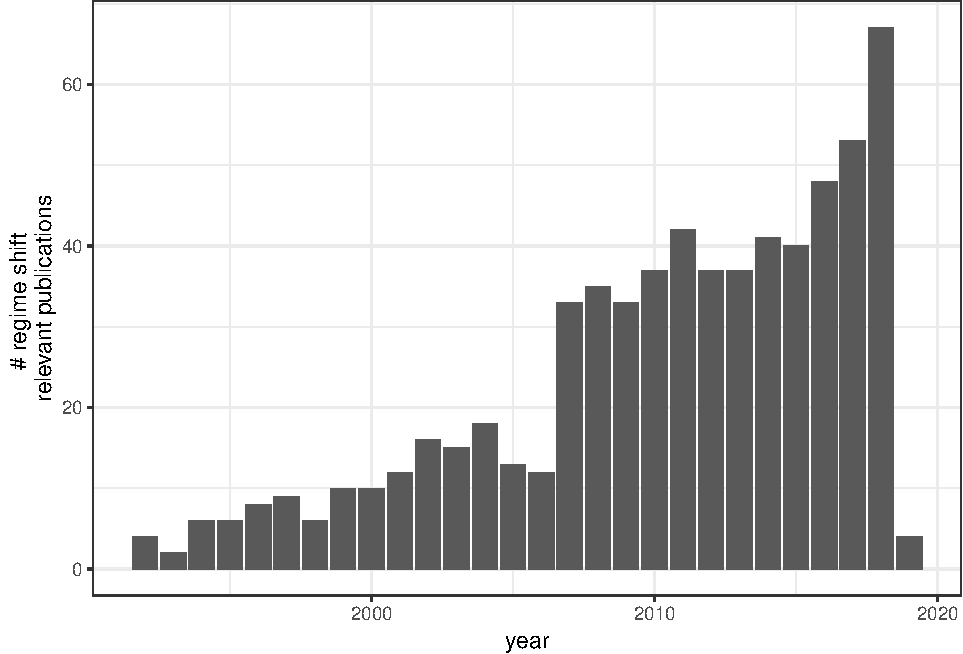
\includegraphics[width=0.85\linewidth]{_myDissertation_files/figure-latex/wosRegimePubsByYear-1} 

}

\caption{Number of publications by year in fields 'Ecology' and 'Biodiversity Conservation' which included terms related to 'regime shift' (total = 654).}\label{fig:wosRegimePubsByYear}
\end{figure}
\hypertarget{results}{%
\section{Results}\label{results}}
\begin{figure}

{\centering 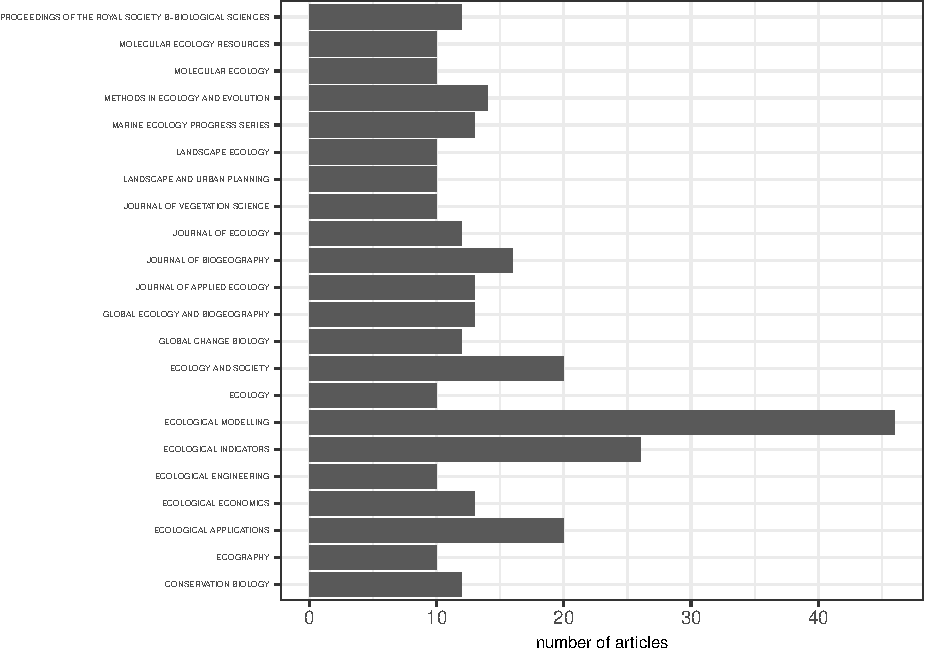
\includegraphics[width=0.85\linewidth]{_myDissertation_files/figure-latex/wosRegimePubsByJrnlmin10Pubs-1} 

}

\caption{Distribution of the 'regime shift' articles for journals with at least 10 articles.}\label{fig:wosRegimePubsByJrnlmin10Pubs}
\end{figure}
\hypertarget{web-of-science-1}{%
\subsection{Web of Science}\label{web-of-science-1}}

The search boolean for WoS boolean \emph{not} including restriction to fields (WC) `Ecology' and `Conservation Biology' yielded over 20,000 results. Restricting to the abovementioned fields created a manageable database from which to filter. This search yielded 2,776 articles. 654 of these papers included terms relating to `regime shifts' (Figure \ref{fig:wosRegimePubsByYear}), many appearing in the journal \emph{Ecological Modelling} (Figure \ref{fig:wosRegimePubsByJrnlmin10Pubs}). The rate of publication of `regime shift' articles is not strongly correlated with the rate of papers published in `Ecology' and `Biodiversity Conservation' fields (Figure \ref{fig:wosRegimePubsByYearwithNumEcolPubs}).
\begin{figure}

{\centering 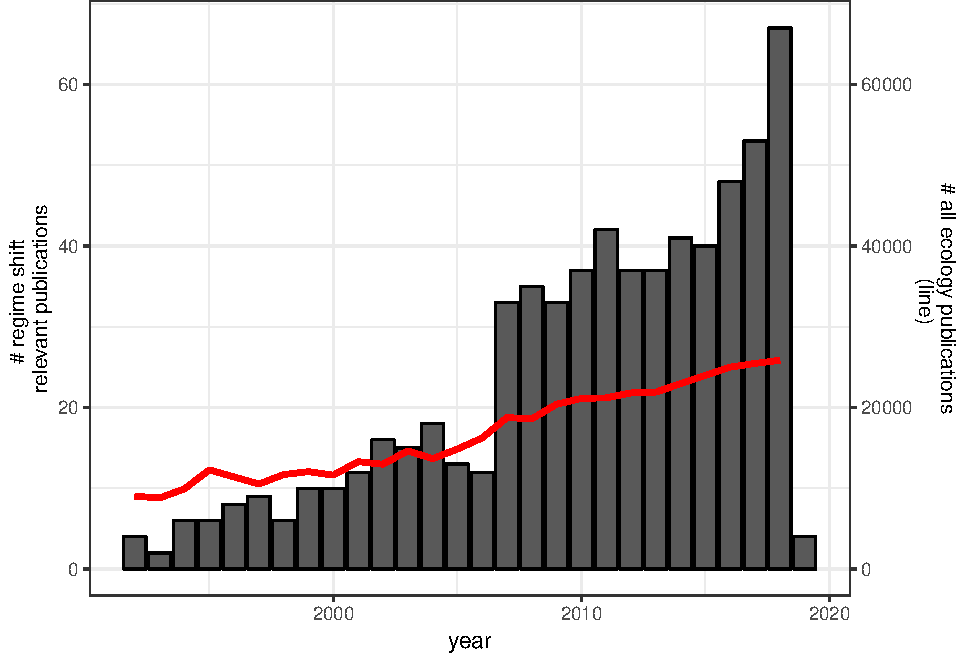
\includegraphics[width=0.85\linewidth]{_myDissertation_files/figure-latex/wosRegimePubsByYearwithNumEcolPubs-1} 

}

\caption{Number of publications by year in fields 'Ecology' and 'Biodiversity Conservation' which included terms related to 'regime shift' (total = 654).}\label{fig:wosRegimePubsByYearwithNumEcolPubs}
\end{figure}
Filtering this WoS results to include only articles mentioning terms related to `new method' yielded 202 articles. After removing prior knowledge, only 93 articles remained to be reviewed `by hand' (i.e., reading the entire paper). Only 2 `new' methods were identified from the WoS search (\ref{fig:rdmReviewFlow}).

\hypertarget{google-scholar-and-prior-knowledge}{%
\subsection{Google Scholar and prior knowledge}\label{google-scholar-and-prior-knowledge}}

Of the 250 articles scanned in Google Scholar, I retained 3 methods. I was previously aware of an additional 68 articles containing `new' methods (\ref{fig:rdmReviewFlow}).
\begin{figure}

{\centering \includegraphics[width=0.85\linewidth]{_myDissertation_files/figure-latex/rdmReviewFlow-1} 

}

\caption{Flowchart of the litearture review process for identifying new regime detection methods. *Only the first ten pages (250 articles) of Google Scholar results were examined. Node shapes: folder = unfiltered articles; box = articles actively filtered; diamond = number of articles with new methods.}\label{fig:rdmReviewFlow}
\end{figure}
\hypertarget{list-of-new-methods}{%
\subsection{List of new methods}\label{list-of-new-methods}}
\begin{longtable}{lll}
\caption{\label{tab:methodsMetricsListTab1}Longtable}\\
\toprule
method & type1 & label2\\
\midrule
\endfirsthead
\caption[]{\label{tab:methodsMetricsListTab1}Longtable \textit{(continued)}}\\
\toprule
method & type1 & label2\\
\midrule
\endhead
\
\endfoot
\bottomrule
\endlastfoot
Autocorrelation at-lag-1 & metric & @vincent1998technique\\
Autoregressive coefficient of AR(1) & metric & @held2004detection\\
Inverse of AR(1) coefficient & metric & @carpenter2008leading\\
Detrended fluctuation analysis & metric & @livina2007modified\\
Spectral density & metric & @kleinen2003potential\\
\addlinespace
Spectral ratio & metric & @biggs2009turning\\
Spectral exponent & metric & @andersen\_ecological\_2009\\
Standard deviation & metric & @carpenter2006rising\\
Coefficient of variation (CV) & metric & @carpenter2006rising\\
Skewness & metric & @guttal2008changing\\
\addlinespace
Kurtosis & metric & @biggs2009turning\\
Conditional heteroskedasticity & metric & @seekell2011conditional\\
BDS test & metric & @carpenterBrock2011early\\
Time-varying AR(p) model & model & @ives2012detecting\\
Nonparametric drift-diffusion-jump model & model & @carpenter2011early\\
\addlinespace
Potential analysis & model & @ives2012detecting\\
Fourier Analysis & NA & @carpenter2010early\\
T-test & metric & @ducre2003comparison\\
Bayesian approaches & model & @jo2016bayesian\\
Mann-whitney U-test & metric & @mauget2003multidecadal\\
\addlinespace
Wilcoxon rank-sum & metric & @karl1987approach\\
Pettitt test & metric & @pettitt1979non\\
Mann-Kendall test & metric & @goossens1987recognize\\
LePage test & metric & @yonetani1993detection\\
Standard normal homoegeneity & metric & @alexandersson1986homogeneity\\
\addlinespace
Regression-based models & model & @solow1987testing\\
Oerleman's method & metric & @oerlemans1978objective\\
Cumulative deviation test (CUSUM) & metric & @buishand1982some\\
Signal-to-noise ratio & metric & @NA\\
Intervention Analysis & metric & @francis1994decadal\\
\addlinespace
STARS & metric & @buishand1982some\\
MCMC & NA & @NA\\
Quickest detection method (Shiryaev<d0>Roberts statistic) & metric & @moustakides2009numerical\\
Variance Index & metric & @brock\_variance\_2006\\
Spectrum indicator & metric & @NA\\
\addlinespace
Wavelet analysis (decomposition) & NA & @cazelles2008wavelet\\
Downton-Katz test & metric & @karl1987approach\\
Rodionov method & metric & @rodionov\_sequential\_2005\\
Nikiforiv method & metric & @NA\\
Average standard deviates & metric & @ebbesmeyer19911976\\
\addlinespace
Fisher Information & metric & @fath\_regime\_2003\\
Vector-autoregressive method & NA & @solow\_test\_2005\\
Lanzante method & NA & @lanzante1996resistant\\
Free-knot splines \& piecewise linear modelling & NA & @gal2010novel\\
Self-exciting threshold autoregressive state-space model SETARSS(p) & model & @tong1990nonlinear\\
\addlinespace
Smooth transition autoregressive model & model & @see gal2010novel\\
Moving detrended fluctuation analysis (MDFA) & metric & @he2008new\\
Nearest-neighbor statistics & metric & @pawlowski\_identification\_2008\\
Clustering, various & NA & @NA\\
dimension reduction techniques (e.g., PCA) & metric & @NA\\
\addlinespace
Sequential tests/moving windows & metric & @NA\\
Online dynamic linear modelling +  time\_varying autoregressive state\_space models (TVARSS) & models & @parparov2017quantifying\\
Stability Index of the Ecological Units & metric & @parparov2015quantifying\\
Generalized model & model & @lade2012early\\
Threshold Indicator Taxa ANalysis (TITAN) & metric & @baker2010new\\
\addlinespace
Convex model & model & @qi2016resilience\\
Probability density function entropy method & metric & @pawlowski\_identification\_2008\\
Method 1-TBD & NA & @manly2006two\\
method-fuzzy synthetic evaluation (FSE) & NA & @wang2011application\\
Method 2-TBD & NA & @manly2006two\\
\addlinespace
Zonal thresholding & metric* & @yin2017methods\\
Characteristic length scale (CLS) estimation & attractor reconstruction & @NA\\
two-phase regression & metric of a model & @easterling1995new\\
shiftogram & model & @groger2011analyses\\*
\end{longtable}
Using my prior knowledge of the relevant litearture, referring to previous review articles, and searching both Web of Science and Google Scholar, I identified 64 unique RDMs (Figure \ref{fig:rdmReviewFlow}; Table \ref{methodsMetricsListTab1}).
\begin{figure}

{\centering 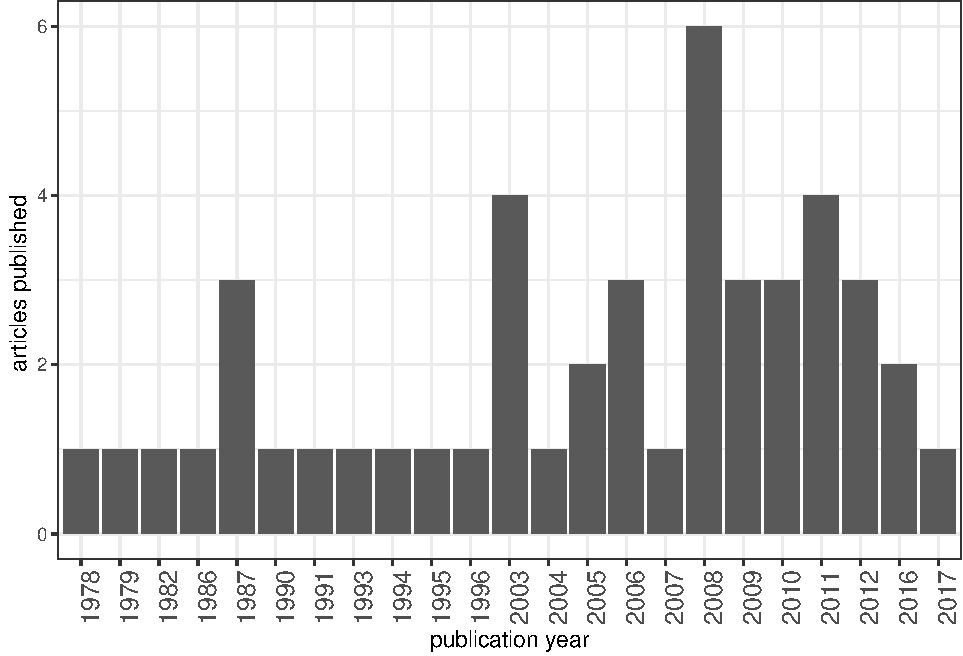
\includegraphics[width=0.85\linewidth]{_myDissertation_files/figure-latex/jrnlYearFig-1} 

}

\caption{Number of methods publisheed over time.}\label{fig:jrnlYearFig}
\end{figure}
\hypertarget{discussion}{%
\section{Discussion}\label{discussion}}

In this chapter I highlighted the plethora of regime detection metrics (RDMs) proposed in the literature for analyzing ecological data (Table \ref{methodsMetricsListTab1}). Although multiple reviews of RDMs exist, they are not comprehensive in their survey of the possible methods. Most reviews have summarized various aspects of RDMs. For example, Roberts et al. (2018) summarizes methods capable of handling multiple (c.f. a single) variable, and Dakos et al. (2015b) review only methods designed to detect the phenomenon of critical slowing down. Here, I did not discriminate--rather, I present an exaustive list of the plethora of methods proposed for detecting ecological detect regime shifts, \emph{sensu lato}, providing a much-needed update to collection provided by S. N. Rodionov (2005), and other review papers (Mac Nally et al., 2014, pp. @scheffer2015generic, @rodionov\_brief\_2005, @roberts2018early, @dakos2015resilience, @mantua\_methods\_2004, @litzow\_early\_2016, @kefi2014early, @andersen\_ecological\_2009, @boettiger\_early\_2013, @dakos\_resilience\_2015, @clements2018indicators, @filatova2016regime, @deyoung\_regime\_2008).

\hypertarget{barriers-to-identifying-new-rdms}{%
\subsection{Barriers to identifying new RDMs}\label{barriers-to-identifying-new-rdms}}

Clearly, as was shown in this chapter (Figure \ref{fig:rdmReviewFlow}), a systematic review of the ecological literature will likely not yield anywhere near a comprehensive list of the RDMs proposed and/or used. This disaparity may be due to both my search methods and to the current state of regime shift research in ecology.

First, my review restricted articles to articles suggesting they were introducing a `new method' as n RDM. Avoiding this potential barrier would have required I review the titles, abstracts, and bodies of over 22,000 articles (Figure \ref{fig:rdmReviewFlow}). Alternatively, this may also be ameliorated by searching the relevant literature for \emph{applications} of RDMs to ecological data, however, I suspect this would similarly yield a large number of articles to review.

Next, only a handful of methods have been introduced to the mainstream methodological journals in ecology (e.g., \emph{Ecological Modelling}, \emph{Methods in Ecology and Evolution}; Figure \ref{fig:jrnlDistFig}). Although many mainstream publications (e.g., \emph{Science}, \emph{Ecology Letters}) include applications of some of the methods identified in this chapter (Table \ref{methodsMetricsListTab1}), I argue that celebrity and `new and shiny' (Steel, Kennedy, Cunningham, \& Stanovick, 2013) methods may influence which methodological articles are printed in these popular journals.
\begin{figure}

{\centering 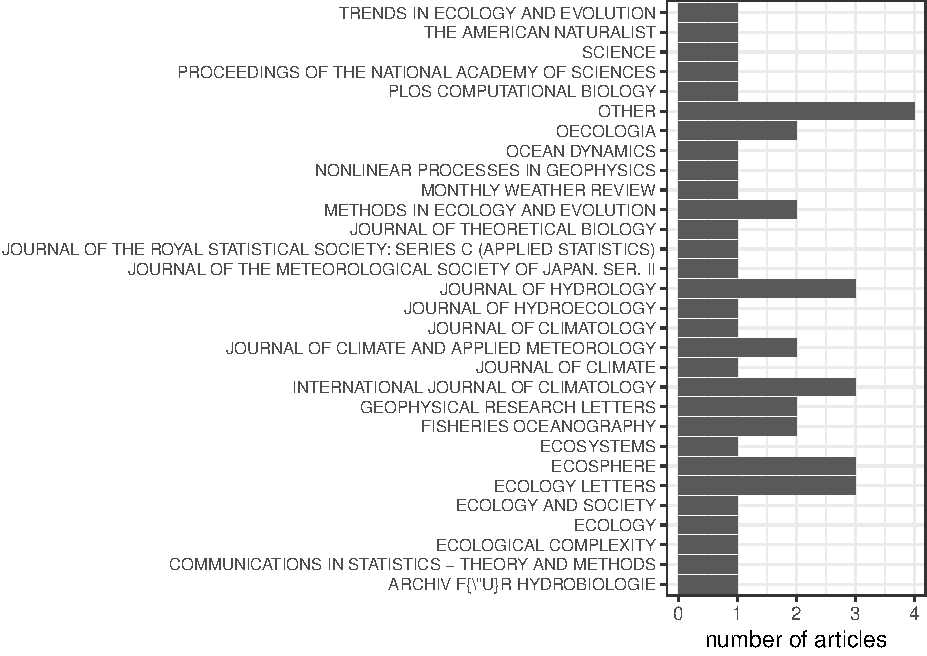
\includegraphics[width=0.85\linewidth]{_myDissertation_files/figure-latex/jrnlDistFig-1} 

}

\caption{Distribution of identified methods across publications. Note: books, reports, and articles without original reference coded as 'Other'}\label{fig:jrnlDistFig}
\end{figure}
A critical survey of potetial and realized applications of these methods would be useful for highlighting the needs of future research and methodological improvements. Many of the methods presented in Table \ref{methodsMetricsListTab1} have either not been applied to empirical data at all, or were tested only once (often but not always in the article introducing the method). Some methods, especially those dubbed `early warning indicators' (variance, autoregressive model coefficients) have become relativley mainstream in their application to empirical data, however, have been shown to be less robust to noisy and nonlinear systems data (Burthe et al., 2016) and systems not exhibiting catstrophic shifts (Dutta, Sharma, \& Abbott, 2018). Most other methods have yet to be rigorously tested on noisy, high dimensional, empirical data. Further, the methods which are not mainstream but have been applied to one of these data types have not any statistical indicators associated with confirming the existence and location of the regime shift.

As shown this chapter, identifying RDMs using traditional literature review techniques may prove difficult. Many of the methods identified in my review were not identified using Web of Science or Google Scholar--rather, I was either previously aware of most of the methods, and many others were highlighted in previous RDM reviews {]}. To facilitate this process, an online, comprehensive database may prove useful to the practical ecologist.

\hypertarget{reducing-the-barriers-to-rdms}{%
\subsection{Reducing the barriers to RDMs}\label{reducing-the-barriers-to-rdms}}

To make the regime detection methods (RDMs) more available and transparent to the practical ecologist, I recommend the following:
1. consitent use of fewer methods
1. persistent collection and maintenance of baseline data (reference data)
1. an on-line database of all RDMs
- open-sourced
- linked to the original sources (in ecology and statistics or mathematics)
- linked to applications
1. a critical review of the current state of RDMs in ecology
- including methodological advancements
- especially highlighting where the method fails to perform
- including historical tracking of specific methods to identify which may need to be retired, rather than resuscitated
1. more empirical applications of these methods (especially of those only tested on toy and experimental data)
1. relation of RDMs in ecology to other fields (computer science, data science, climatology and oceanography)

I suggest below a suite of questions which may provide useful in a critical review of the characteristics, rigor, and promise of RDMs in the context of ecological data analysis.
\begin{longtable}{>{\bfseries}l|>{\raggedright\arraybackslash}p{30em}}
\caption{\label{tab:nextStepsTab}Potential questions for a comprehensive review of the ecological regime detection metrics literature.}\\
\toprule
Type & Questions\\
\midrule
Methodological & What are the major assumptions about the distribution?\\
 & Does the method explicitly assume stationarity? If not, can it handle non-stationary processes?\\
 & Does the performance of the method change with non-stationarity?\\
 & Can the method handle unstructured data (information)?\\
 & Does the regime shift need to be identified *a priori*?\\
\addlinespace
 & Can the method handle multiple regime shifts?\\
 & Does the performance of the method change with non-stationarity?\\
 & What types of regime shifts can the method detect (e.g., stochastic resonance, slow-fast cycles, noise-induced transition)?\\
 & Is it a model- or metric-based method?\\
 & Does it have forecasting potential?\\
\addlinespace
 & Can the method handle uneven sampling?\\
 & What are the minimum data requirements (resolution, extent, number of observations)?\\
 & How does the method handle missing data (e.g., new invasions)?\\
 & Does the method assume Eulerian or Lagrangian processes?\\
Ecological & Has the method been tested on empirical data? If so, to what rigor?\\
\addlinespace
 & What is the impact of losing state variables on long-term predictions (e.g., species extinction)?\\
 & Can the method identify drivers?\\
 & What assumptions does the method make about the system?\\
 & What types of regime shifts are possible in the system?\\
 & Are regime shift(s) suspected *a priori*?\\
\addlinespace
 & What lag(s) exist in the data (system)?\\
 & Would a positive forecast change management action?\\
 & Do predictions translate to other systems?\\
 & Can we interpolate data if necessary? If so, what does this mean for inference?\\
 & In which discipline(s) beyond ecology has the method been tested?\\
\bottomrule
\end{longtable}
\hypertarget{fiGuide}{%
\chapter{A guide to Fisher Information for Ecologists}\label{fiGuide}}

\emph{This chapter is intended for submission to the publication \emph{Methods in Ecology and Evolution}.\footnote{Co-authors include: N.B. Price, A.J. Tyre, C.R. Allen, T. Eason, D.G. Angeler, and D. Twidwell}}

\hypertarget{abstract-1}{%
\section{Abstract}\label{abstract-1}}

Ecological regime shifts are increasingly prevalent in the Anthropocene. The number of methods proposed to detect these shifts are on the rise yet few are capable detecting regime shifts without a priori knowledge of the shift or are capable of handling high-dimensional and noisy data. A variation of Fisher Information (FI) in a dataset was proposed as a method for detecting changes in the orderliness of ecological systems. Although FI has been described in multiple research articles, previous presentations do not highlight a key component of FI that may make the metric easier to understand by practitioners. We use a two-species predator prey model to describe the concepts required to calculate FI. We hope this work will serve as a useful explanation of the FI metric for those seeking to understand it in the ecological systems and regime shifts.

\hypertarget{introduction-1}{%
\section{Introduction}\label{introduction-1}}

Changes in the feedback(s) governing ecosystem processes can trigger unexpected and sometimes undesirable responses in environmental conditions (Scheffer, Carpenter, Foley, Folke, \& Walker, 2001; Walther et al., 2002). Ecologists often refer to such changes as regime shifts, but this term is used interchangeably in the literature with state change, state transition, or alternative state (Andersen et al., 2009). Climate change and globalization are triggering novel and unexpected changes in ecosystems, and the rapidity with which these changes occur make predictive modeling difficult. Although detecting regime shifts becomes more difficult as we increase the extent and complexity of the system in question , advances in the collection and analysis of ecological data may improve our ability to detect impending regime shifts in time for intervention (Jorgensen \& Svirezhev, 2004).

Although multiple quantitative approaches are proposed as regime shift detection methods ,few are consistently applied to terrestrial ecological data. We classify a regime shift detection methods (DMs) broadly as either model-based or model-free (Boettiger \& Hastings, 2012; Dakos et al., 2012; Hastings \& Wysham, 2010). Model-based methods incorporate mathematical (mechanistic) representations of the system (Hefley, Tyre, \& Blankenship, 2013) and carry strict assumptions, which are often violated by real systems (Abadi, Gimenez, Arlettaz, \& Schaub, 2010). In addition to assumption violations nullifying parts of the model, model misspecification may yield spurious results {[}Perretti, Munch, \& Sugihara (2013).

Model-free (or metric-based detectin ethods (e.g., descriptive statistics, cross-correlation mapping) require fewer assumptions to implement than do model-based DMs (Dakos et al., 2012). The most widely used model-free methods for detecting ecological regime shifts include descriptive statistics of one or a few components of a system, such as variance, skewness, and mean value (Andersen et al., 2009; Mantua, 2004; S. Rodionov \& Overland, 2005) and composite measures which handle multivariable data, including principal components analysis (Petersen et al., 2008), clustering algorithms (Beaugrand, 2004), exergy (Fath \& Cabezas, 2004), and Fisher Information (Cabezas \& Fath, 2002; Karunanithi, Cabezas, Frieden, \& Pawlowski, 2008).

Fisher Information, hereafter FI is a model-free composite measure of any number of variables (Fisher, 1922), and is proposed as an early warning signal for ecological regime shift detection system sustainability (Mayer, Pawlowski, Fath, \& Cabezas, 2007, p. @karunanithi\_detection\_2008, Eason and Cabezas 2012, Eason et al.~2014a). Three definitions of FI exist:
I. A measure of the ability of the data to estimate a parameter.\\
II. The amount of information extracted from a set of measurements (Roy Frieden, 1998).\\
III. A measure representing the dynamic order/organization of a system (Cabezas \& Fath, 2002).

The application of FI to complex ecological systems was posed as part of the `Sustainable Regimes Hypothesis,' stating a system is sustainable, or is in a stable dynamic state, if over some period of time the average value of FI does not drastically change (Cabezas \& Fath, 2002). This concept can be described using an ecological example. Consider the simple diffusion of a population released from a point source at \(t = 0\). This process can be described by a bivariate normal distribution, \(p(x,y\vert t)\). As the time since release (as \(t\) increases) increases the spread of the distribution, \(p(x,y\vert t)\), becomes larger (less concentrated about the mean) because the animals have moved further from the release location. FI will decrease in value as t increases, because \(p(x,y\vert t)\) contains less information (higher uncertainty) about where the animals will be located. As \(t \rightarrow \infty\), the animals will be relatively uniformly distributed across the environment and \(p(x,y\vert t)\) will carry no information about the location of the animals. Consequently, as \(t \rightarrow \infty\), FI will approach zero. This system is not in a stable dynamic state because FI is decreasing with time.

In contrast, imagine a population varying around a carrying capacity following a simple logistic growth model. As long as the average system parameters (r and K and their variances) are stationary (not changing with time), then the logarithm of population size will have a normal distribution (check this!!!might need some different model). The FI measured over any selected window of time will be constant, indicating that the system is in a stable dynamic state. A perturbation to the population size due to disturbance will also not affect FI, as long as the disturbance does not change the distributions of r and K, and the perturbations themselves occur with some stationary probability distribution.

Although the concept of FI is firmly grounded in physics (Frieden, 1998), the concepts behind its application to ecological systems remain elusive to the average ecologist. We aim to elucidate the statistical concept of FI and the steps required to calculate it as a measure of `ecosystem order' and as a regime shift detection method (Cabezas \& Fath, 2002; Fath, Cabezas, \& Pawlowski, 2003). We believe a concise and accessible synthesis of the topic, along with reproducible code, will aid the ecologists' understanding of this metric and will advance our understanding of its usefulness as an indicator of ecological regime shifts. We reproduce the analyses presented in (Fath et al., 2003) and Mayer et al. (2007) to fully explain these concept of and steps for calculating this form of Fisher Information. We hope this work will serve as a useful explanation of the FI metric for those seeking to understand it in the ecological regime shift context and will stimulate research using this and other multivariate, model-free, and composite measures to understand ecological regime shifts.

\hypertarget{on-fisher-information}{%
\subsection{On Fisher Information}\label{on-fisher-information}}

Two methods exist for calculating Fisher Information (FI) as applied to ecological systems data, which we refer to as the \emph{derivatives-based} method, first appearing in Cabezas \& Fath (2002), and the \emph{binning} method, first appearing in Karunanithi et al. (2008). The binning method was proposed as an alternative to the derivatives-based method for handling noisy and sparse data, and requires additional calculations and system-specific decisions, and for these reasons we focus solely on the derivatives-based method. The general form of FI can be found in (Fath et al., 2003) and (Mayer et al., 2007), and although others can be found, we refer the reader to Cabezas \& Fath (2002) for a complete derivation of FI, and to @ref(\#fiBiblio) for applications of Fisher Information in other fields.

\hypertarget{notation}{%
\subsection{Notation}\label{notation}}

A capital letter (e.g., \(A\)) denotes a random variable; an asterisk superscript (\(^*\)) indicate a particular realization; \emph{bold notation} indicates that the state of the system is defined in more than one dimension.

\hypertarget{steps-for-calculating-fisher-information-fi}{%
\subsection{Steps for calculating Fisher Information (FI)}\label{steps-for-calculating-fisher-information-fi}}

To calculate FI for a system with more than one state variable, we first estimate the probability of observing the system \(p(x)\) in a given state, \(x\), over time period \(T\). The probability density function, \(p(x)\), is then directly used to calculate the derivatives-based FI. We use bold notation to indicate that the state of the system is defined in more than one dimension (e.g., the state of a predator prey system is defined in two dimensions by the number of predators and number of prey). Here, we describe these steps and present the numerical calculation of FI using a two-species predator-prey model {[}Fath et al. (2003); mayer\_applications\_2007{]}, hereafter referred to as the `model system':
\begin{equation} 
  dx_1 = g_{1}x_{1}(1-\frac{x_1}{k})- \frac{l_{12} x_{1} x_{2}}{1+\beta x_{1}} \\
  dx_2 = \frac{g_{21}x_1 x_2}{1+\beta x_1} - m_2 x_2)
  \label{eq:predprey}
\end{equation}
The specified parameters for the model system are \(g_1=m_2=1\), \(l_12=g_12 = 0.01\) , \(k=625\) ,and \(\beta=0.005\) (see Fath et al., 2003; Frieden \& Gatenby, 2007; Mayer et al., 2007). The initial conditions (predator and prey abundances) for the model system were not provided in the original references. Using package \emph{deSolve} in Program R (v 3.3.2) to solve the model system \eqref{eq:predprey} we found \(x_1 = 277.7815\) and \(x_1= 174.551\) provided reasonable results. We found that a complete cycle of the system corresponds to approximately 11.145 time units.
\begin{figure}

{\centering 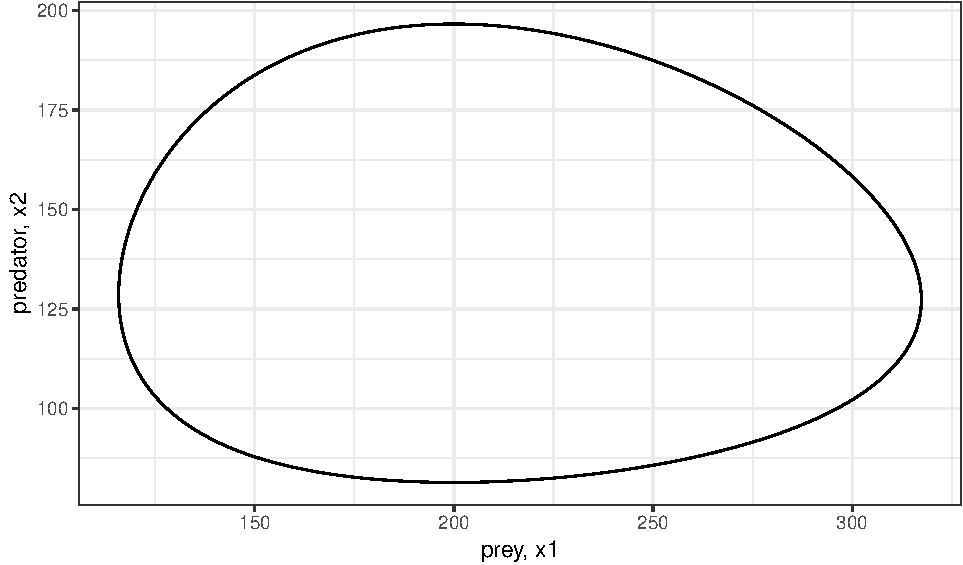
\includegraphics[width=0.85\linewidth]{_myDissertation_files/figure-latex/pp1Period-1} 

}

\caption{Phase space plot of two-species Lotka-Volterra predator-prey system over a single period (~11.145 time units.}\label{fig:pp1Period}
\end{figure}
\hypertarget{concepts-behind-the-calculations}{%
\subsection{Concepts behind the calculations}\label{concepts-behind-the-calculations}}

Although the numerical steps for calculating the derivatives-based FI are relatively straightforward, the concepts required to interpret the measure in the context of multiple variables is more complex. Here, we thoroughly discuss the concepts and assumptions behind FI calculation. Below, steps do not represent steps within the calculation, they represent the major concepts required

\hypertarget{step-1.-probability-of-observing-the-system-in-a-particular-state-px}{%
\subsubsection{\texorpdfstring{\textbf{Step 1. Probability of observing the system in a particular state, \(p(x)\)}}{Step 1. Probability of observing the system in a particular state, p(x)}}\label{step-1.-probability-of-observing-the-system-in-a-particular-state-px}}
\begin{figure}

{\centering 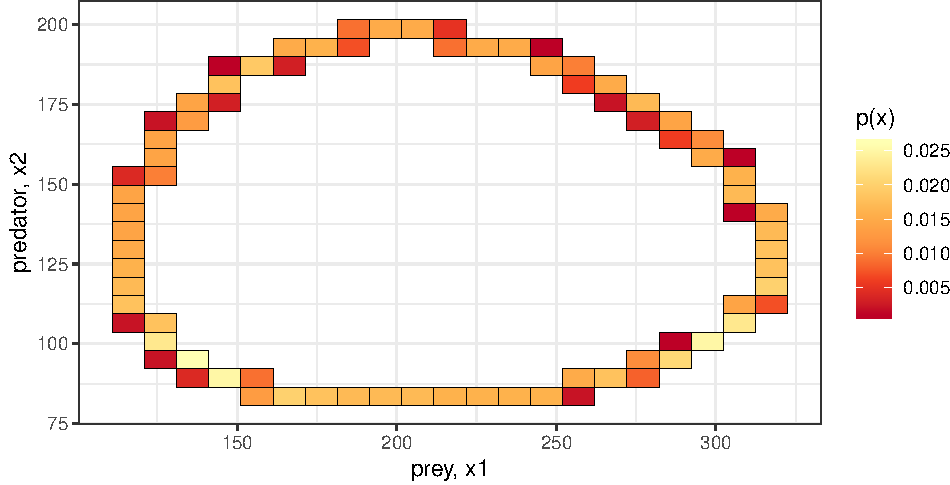
\includegraphics[width=0.85\linewidth]{_myDissertation_files/figure-latex/2D-hist-1} 

}

\caption{A 2-dimensional histogram of the probability of observing a system in a particular state, $p(x)$, of the 2-species Lotka-Volterra predator prey system over a single period (~11.145 time units).}\label{fig:2D-hist}
\end{figure}
Fisher Information (FI) is defined with respect to a probability distribution. In the derivatives-based method, FI is calculated for a probability of observing a system (as defined by one or more state variables) in a particular state, \(p(x)\), over some period of time, (\(0 to t_{end}\)). In other words \(p(x)\) is the probability that, at a specific point in time (\(t_{obs}^*\)) we will observe the system in a particular state, \(x^*\). The time at which we observe the system is a random variable, \(t_{obs} ~ Uniform(0,t_{end})\). To be clear, the study system is assumed to be deterministic and we assume no observation error, however, the observed state of the system, \(x(T_{obs})\), is a random variable because it is a function of the random observation time, \(x^*= x(t_{obs}^*)\). The state of the model system, x, is defined in two dimensions by the number of predators and the number of prey \eqref{eq:predprey} and is easily visualized \ref{fig:pp1Period}.Therefore, the probability of observing a particular state is a two-dimensional joint distribution \ref{fig:2d-hist}.

A single state of the model system is defined by the number of predators and prey at a given point in time such that for any given point in time \(x(t)=[x_1 (t),x_2 (t)]\). At some random time between 0 and \(t_{end}\) {[}\(T_{obs} ~ Uniform(0,t_{end})\){]} we can count the number of predators and the number of prey to determine the state of the model system. We must assume the system is deterministic and there is no observation error. We can then calculate the probability of observing a particular predator and prey abundance combination, \(p(x)\). Under these assumptions, the only possible states of the system are defined by the system's observed trajectory, the model parameters, and the initial conditions. Therefore, the support of the probability distribution \ref{fig:2D-hist} is the trajectory of the system.
\begin{figure}

{\centering 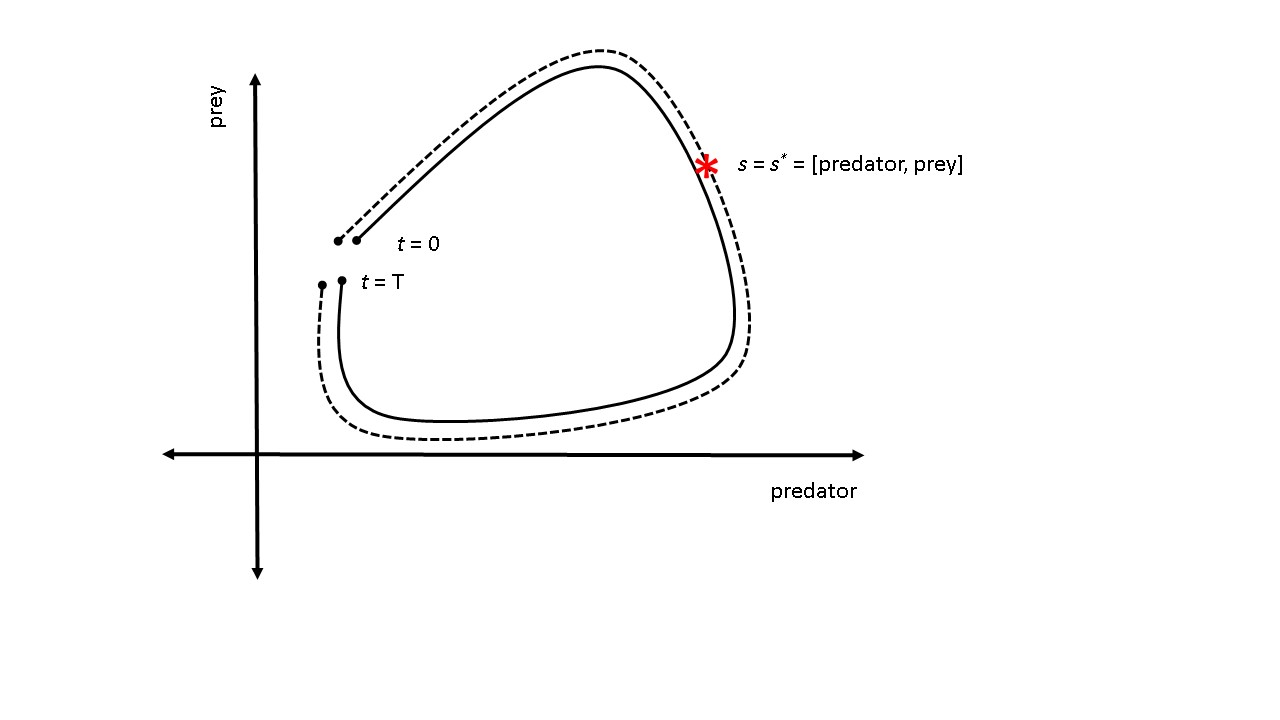
\includegraphics[width=0.85\linewidth]{./chapterFiles/fiGuide/figures/stringFig} 

}

\caption{A single cycle of a hypothetical two-species system over time period $t = 0$ to $t = T$. $s^*$ is the state of the system at some point in time. The dotted line represents the distance travelled by the system in phase space over its trajectory during time $(0, T)$.}\label{fig:stringFig}
\end{figure}
\hypertarget{step-2.-distance-traveled-by-the-system-s}{%
\subsubsection{\texorpdfstring{\textbf{Step 2.} Distance traveled by the system, \(s\)}{Step 2. Distance traveled by the system, s}}\label{step-2.-distance-traveled-by-the-system-s}}

Distance traveled by the system, s. We can now move from an n-dimensional representation of the probability distribution to a one-dimensional representation. To better understand this, imagine placing a string over the path of the entire trajectory from \(0 to t_{end}\) \ref{fig:stringFig}. If we know the number of predators and prey at a particular point in time \((t_{obs}^*)\) then we can mark that location on the string (see asterisk in \ref{fig:stringFig}. Next, imagine picking up the string and laying the string flat along a ruler. The length, s, of the entire string measures the total distance traveled by the system in phase space. The mark we made on the string (denoted \(*\)) lies at a distance \(s^*\) between 0 and \(s\). We call this length the distance traveled by the system, \(s^*\). In this context, \(s^*\) in phase space represents a measure of cumulative change in state. We note that the distance traveled in phase space increases monotonically with time. If the system never revisits the same state (i.e., the trajectory never overlaps or intersects itself), then every unique system state (i.e., point on the trajectory) is mapped to a unique value of distance traveled. Therefore, \(p(x)\) (n-dimensional) is equivalent to the probability that the system is at distance s, i.e., \(p(x)=p(s)\), (where \(p(s)\) is one dimensional; Cabezas, Pawlowski, Mayer, \& Hoagland (2005)). However, if the system revisits previous states, then a unique system state may be mapped to different values of distance traveled and the relationship between \(p(x)\) and \(p(s)\) is not one-to-one. We calculated the distance traveled s of the model system over a single cycle (11.145 time units; \ref{fig:distSpeedAccel}.
\begin{figure}

{\centering 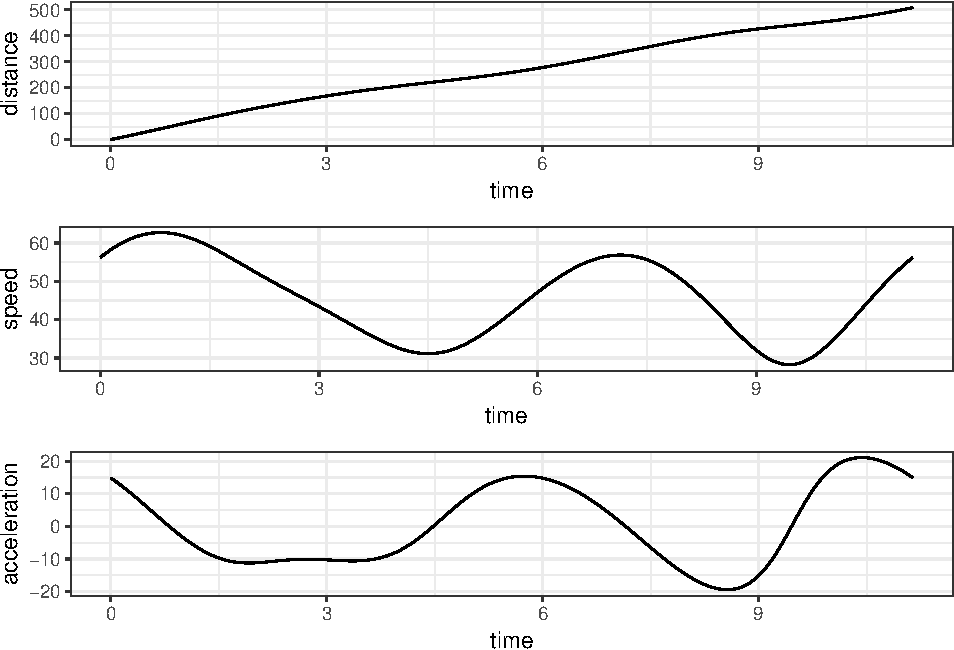
\includegraphics[width=0.85\linewidth]{_myDissertation_files/figure-latex/distSpeedAccel-1} 

}

\caption{From top to bottom, distance traveled in phase space, speed tangential to system trajectory, acceleration tangential to system trajectory.}\label{fig:distSpeedAccel}
\end{figure}
\hypertarget{step-3.-ps-as-a-function-of-the-rate-of-change-of-s}{%
\subsubsection{\texorpdfstring{\textbf{Step 3.} \(p(s)\) as a function of the rate of change of \(s\)}{Step 3. p(s) as a function of the rate of change of s}}\label{step-3.-ps-as-a-function-of-the-rate-of-change-of-s}}

In previous presentations of FI, the relationship between the state of the system (n-dimensional) and the distance traveled (1-dimensional) was not always emphasized (Cabezas \& Fath, 2002). Here we use x to denote the state of the system and s to denote the distance traveled to emphasize this distinction. If a system travels at a constant speed over the entire time period, then the system is equally likely to be in any state along the trajectory (\(s\) is linear and \(p(s)\) is uniform). Referring to our model system, if the number of predators and prey are linearly related, then the speed of the system is constant. For non-linear systems, the distribution above the string will not be uniform \ref{fig:stringFig}. Rather, it will change depending on the amount of time the system spends in each state. It follows that \(p(s)\) is proportional to the inverse of the rate of change of distance traveled (i.e., the speed along the path in phase space).

We will now demonstrate this using our model system as an example. Suppose the abundances of the predator and their prey in our model system predictably operate at carrying capacity. Over a relatively short period of time the prey abundance quickly declines after a severe weather event (a pulse disturbance; (Bender et al.~1984), but quickly recovers. Intuitively, the absolute rate of change at time points near the disturbance will be larger than during time periods long before or long after the disturbance. It is therefore more likely that the system will be (observed) in a state where prey and predators are operating approximately at carrying capacity than in a state with relatively low prey abundance. Mathematically, the time, \(t*\), at which we calculate the abundances of prey and predators is a uniform random variable, and the distance traveled by the system, \(s^*\), is a function of time, is differentiable, and monotonically increases. Therefore, the probability density function of the distance traveled \(p(s)=\frac{1}{T}\frac{1}{s'}\), where \(s'= \frac{ds}{dt}\) is the speed of the system (the speed tangential to the trajectory; the first derivative of the distance traveled; instantaneous rate of change of \(s\)). We calculated the speed (the first derivative; \ref{fig:distSpeedAccel} and acceleration (the second derivative; \ref{fig:distSpeedAccel} of the distance traveled s by the model system over a single cycle using function ode in package deSolve (Soetaert et al.~2010) in Program R (R Core Team 2016).

\hypertarget{step-4.-calculate-the-derivatives-based-fisher-information}{%
\subsubsection{\texorpdfstring{\textbf{Step 4.} Calculate the derivatives-based Fisher Information}{Step 4. Calculate the derivatives-based Fisher Information}}\label{step-4.-calculate-the-derivatives-based-fisher-information}}

Now that we understand how to calculate both the distance traveled, \(s\), and its probability density, \(p(s)\), calculating the derivatives-based FI is straightforward and computationally inexpensive \eqref{eq:fiDerivs}. There are several comparable equations for calculating the shift-invariant FI, and some may offer numerical advantages over others. Equation \eqref{eq:fiAdapted} is the general form and Equation \eqref{eq:fi73c} is the amplitude form for FI (in Mayer et al. (2007), respectively). Although these formulations are equivalent, \eqref{eq:fi73c} is most readily calculated when the differential equations for the system are known, obviating any advantage of a model-free metric.
\begin{equation}   
    I = \frac{1}{T} \int_0^T dt\left[\frac{s''^2}{s'^4}\right]^2 \\  
  \label{eq:fiDerivs}  
\end{equation}
\begin{equation} 
    I = \int \frac{ds}{p(s)}\left[\frac{dp(s)}{ds}\right]^2  \\
    \label{eq:fiAdapted}
\end{equation}
\begin{equation} 
    I = 4 \int ds\left[\frac{dq(s)}{ds}\right]^2 \\
\label{eq:fi73c}
\end{equation}
This article is interested in the Fisher Information calculated for a distribution of distance traveled, \(s\), by the entire system. We calculated the Fisher Information value using Equation \eqref{eq:fiDerivs} over a single period of the model system (\eqref{eq:predprey}). We calculated Fisher Information to be \(5.3\) x \(10^{-5}\) which is consistent with the results of Mayer et al.~(2007).

\hypertarget{case-study}{%
\section{Case Study}\label{case-study}}

Mayer et al.~(2007) calculated FI for a predator-prey system for several discrete values of carrying capacity of prey. The results of this study showed that FI was different for systems with different carrying capacities. However, this study did not address the central question of how FI changes during a regime shift. As an extension of the original study, we simulate a regime shift by modeling a situation where carrying capacity is abruptly decreased. To simulate an abrupt change in carrying capacity, we assume carrying capacity is described by Eq. 6 where \(k1\) is the initial carrying capacity, \(k2\) is the final carrying capacity, \(t*\) is the time of the regime shift, and alpha is a parameter that controls how quickly the regime shift occurs. The hyperbolic tangent function simulates a smooth, continuous change in carrying capacity while still allowing for the change to occur suddenly. To incorporate the change in carrying capacity into the system differential equations we define the rate of change of carrying capacity as given by \eqref{eq:mayerCase}.\\
\begin{equation}  
  k(t) = k_1  - 0.5(k_1-k_2)(\tanh(\alpha (t-t^*))+1)     \\
  k'(t) = 0.5\alpha (k_1-k_2)(\tanh(\alpha(t-t^*))^2 +1)      \\ 
\label{eq:mayerCase}
\end{equation}
\begin{figure}

{\centering 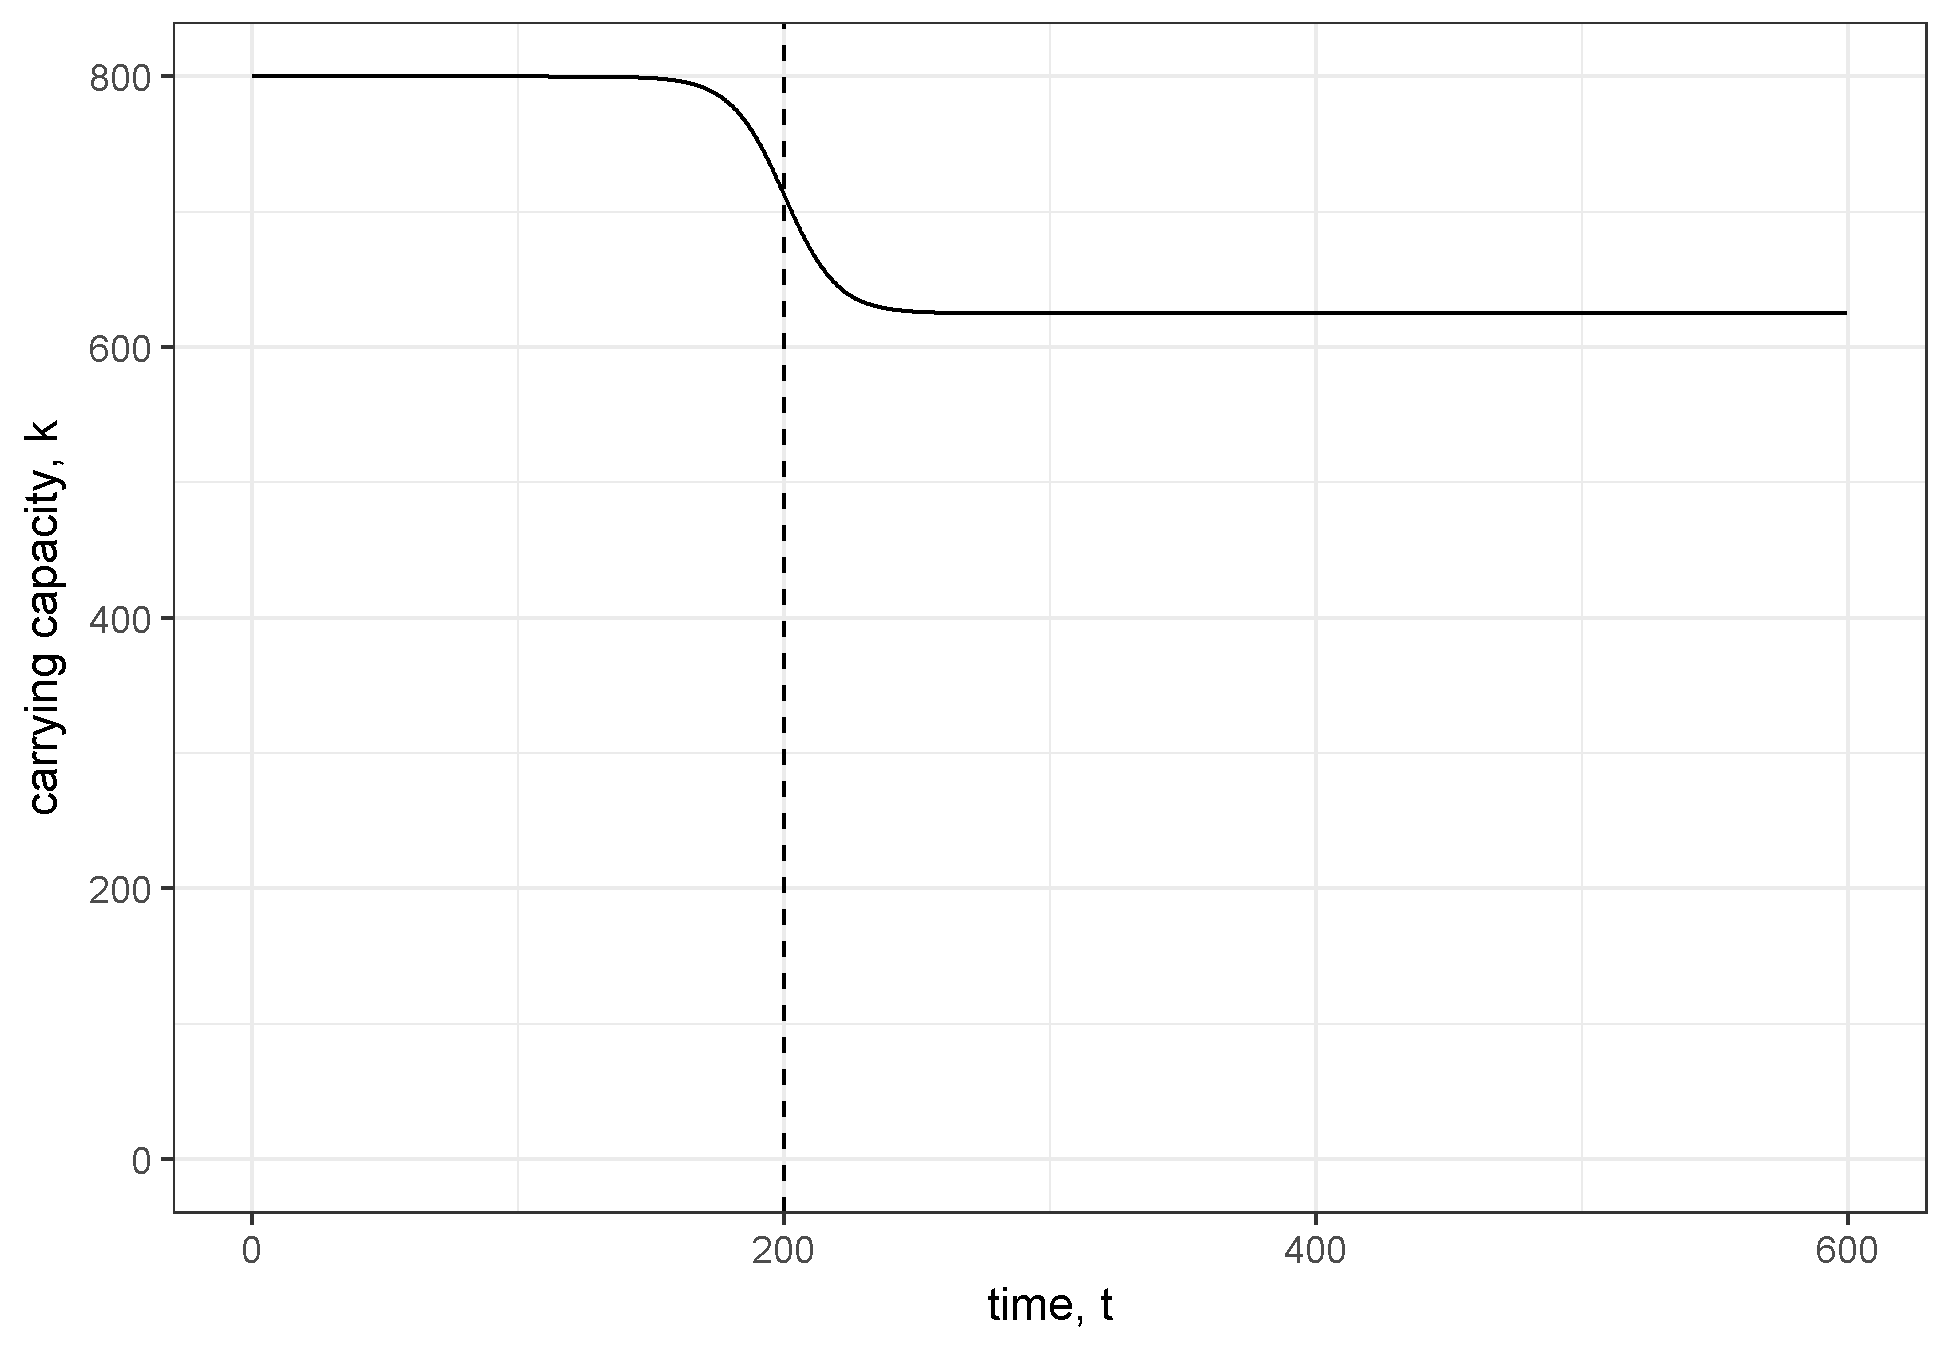
\includegraphics[width=0.85\linewidth]{./chapterFiles/fiGuide/figures/kByTime} 

}

\caption{Carrying capacity over time with a regime shift occuring around time 200.}\label{fig:kByTime}
\end{figure}
\begin{figure}

{\centering 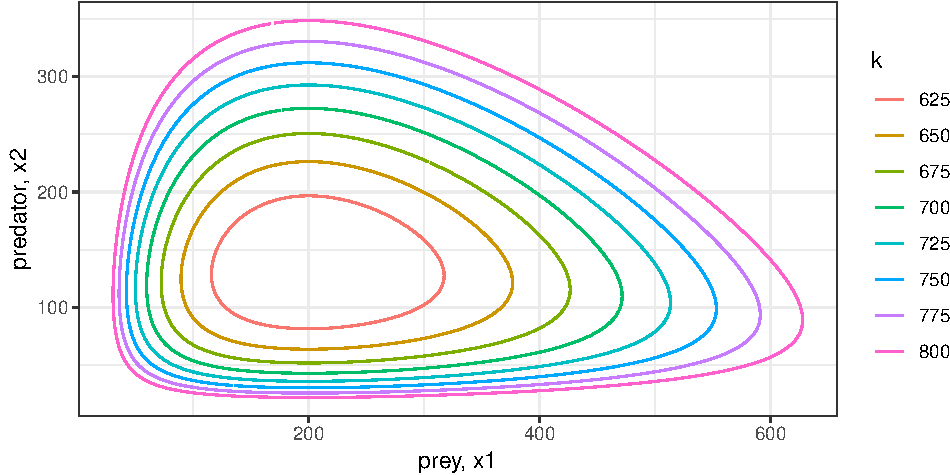
\includegraphics[width=0.85\linewidth]{_myDissertation_files/figure-latex/kTrajectories-1} 

}

\caption{Phase space plot of system trajectories for different values of k}\label{fig:kTrajectories}
\end{figure}
We assumed an initial carrying capacity of 800 and a final carrying capacity of 625 which corresponds to the range of carrying capacities explored by Mayer et al.~(2007). We simulated a time series of 600 time units with a regime change after 200 time units. We used an alpha value of 0.05. The time series for carrying capacity is shown in \ref{fig:kByTime} and the system trajectory in phase space is shown in \ref{fig:kTrajectories}. The distance travelled in phase space (i.e., cumulative change in state) is shown in \ref{fig:distOverTime} and the speed of the system (i.e., rate of change) is shown in \ref{fig:dsdtOverTime}.
\begin{figure}

{\centering 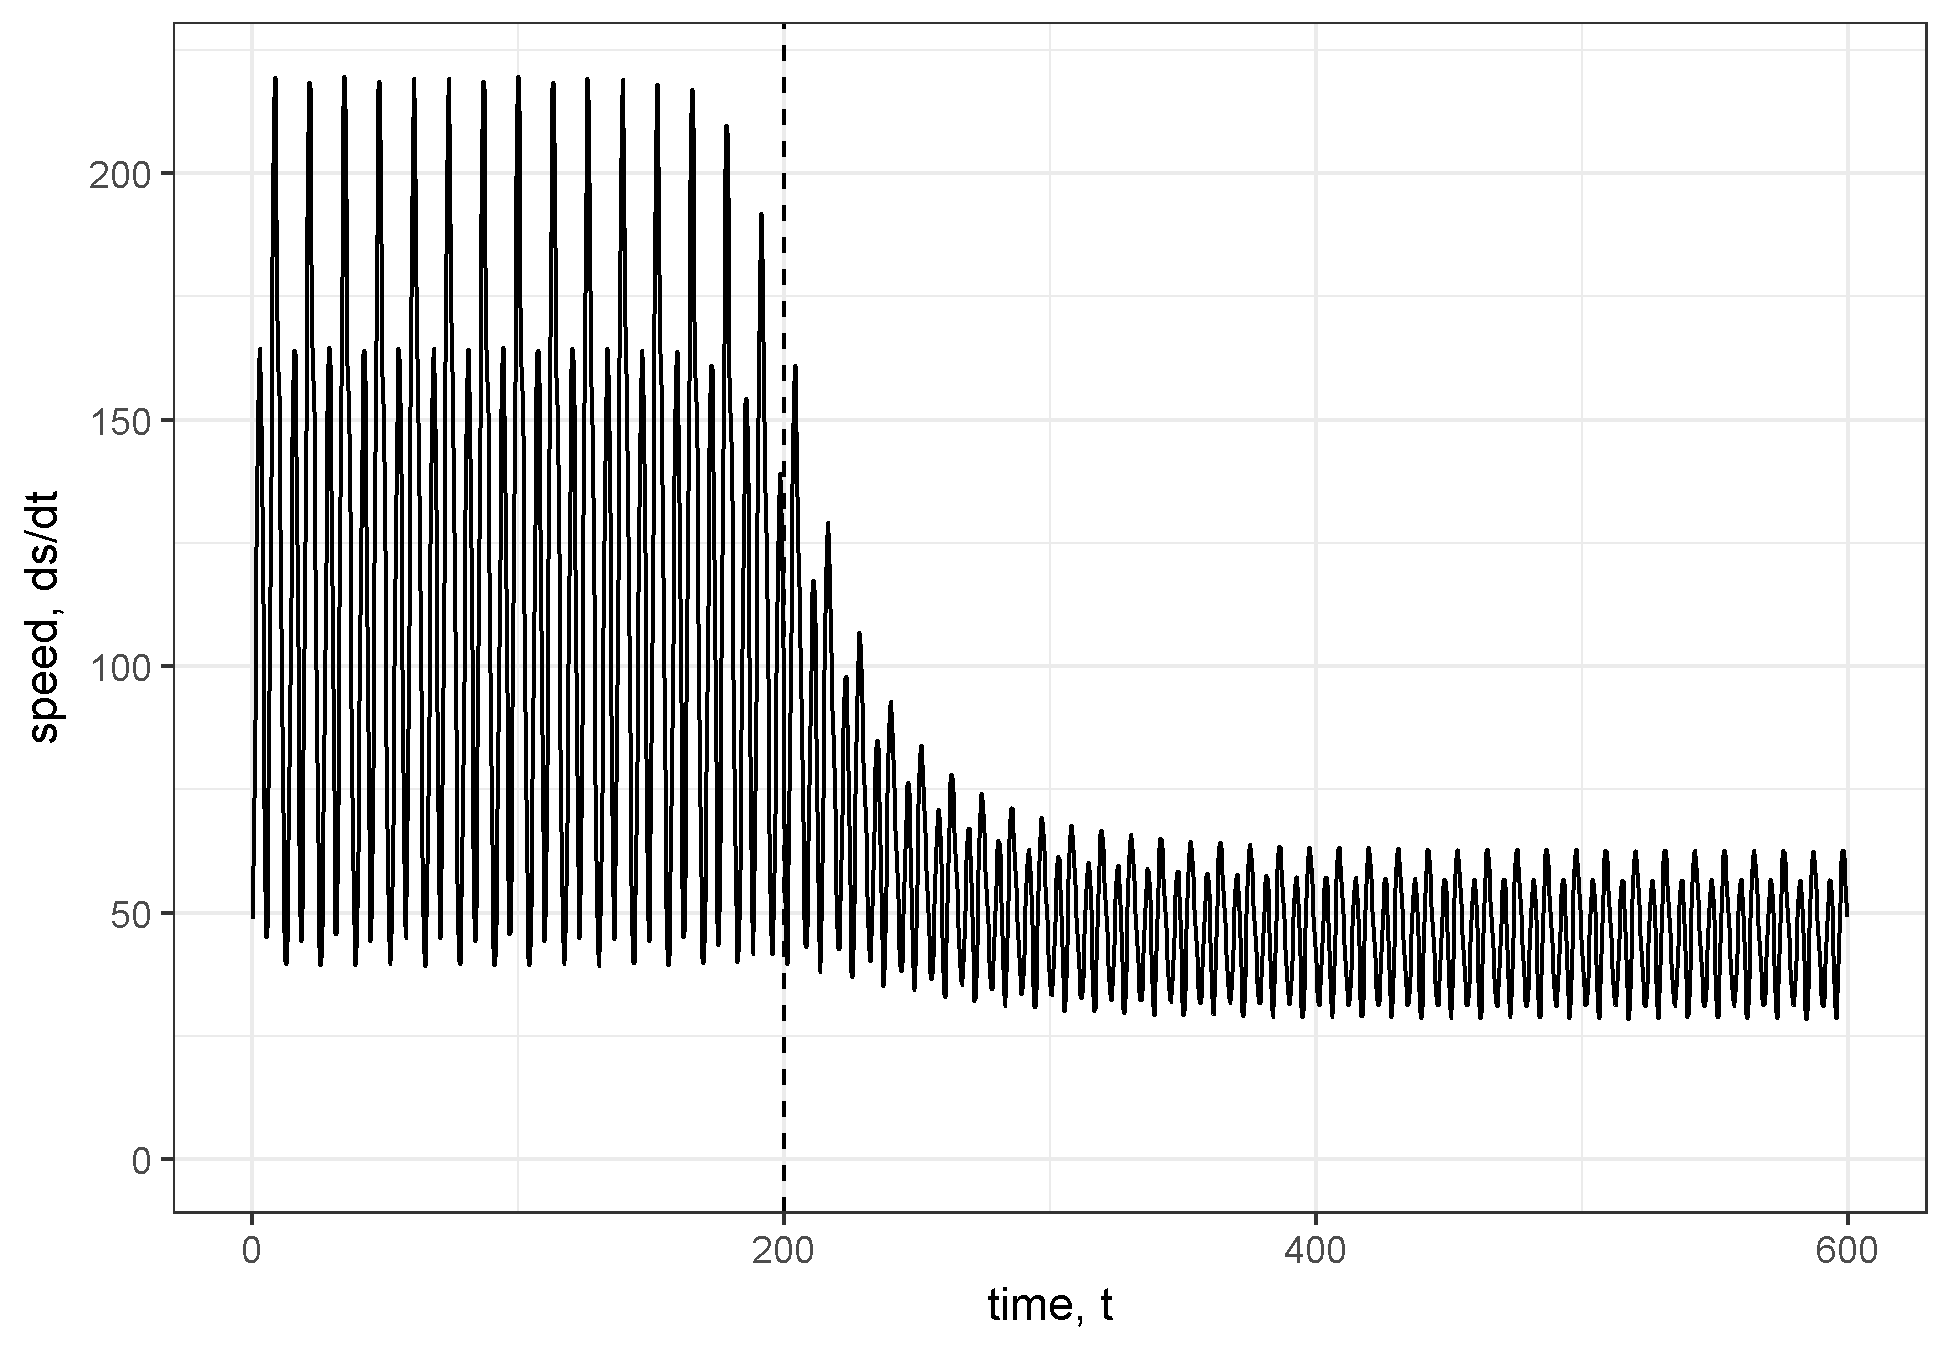
\includegraphics[width=0.85\linewidth]{./chapterFiles/fiGuide/figures/dsdtOverTime} 

}

\caption{Speed of the system (rate of change) in phase space. Dashed vertical line at time 200 indicates location of regime shift.}\label{fig:dsdtOverTime}
\end{figure}
We calculated FI for the distribution of distance travelled over a series of non-overlapping time windows. Multiple sources suggest the length of the time window should be equal to one system period such that FI is constant for a periodic system (Cabezas \& Fath, 2002; Mayer et al., 2007). However, the system period is different before, during, and after the regime shift. Therefore, we performed two separate calculations of FI using window sizes corresponding to the initial and final period of the system (\(13.061\) and \(11.135\), respectively). The change in FI over time is shown in \ref{fig:fiOverTime}.
\begin{figure}

{\centering \includegraphics[width=0.85\linewidth]{./chapterFiles/fiGuide/figures/fiOverTime} 

}

\caption{Fisher Information calculated for non-overlapping time windows. Two different window sizes were used as indicated by color. Dashed vertical line at time 200 indicates approximate location of regime shift.}\label{fig:fiOverTime}
\end{figure}
\hypertarget{conclusions}{%
\section{Conclusions}\label{conclusions}}

We simulated a regime shift caused by a change in carrying capacity (\(K\)) within a simulated, two-species Lotka-Volterra system. We applied the Fisher Information (FI) method for regime shift detection to the simulated time series data. The predator-prey system was modeled as deterministic and the time series data was free from measurement and observation error. Despite this, the estimated FI had high variation over time, and results were dependent on the size of the time window used (winsize) in the calculation \ref{fig:fiOverTime}. The FI method for regime shift detection is based on the cumulative change in the state of the system (i.e., distance traveled in phase space) and the rate of change of the system (i.e., speed tangential to trajectory in phase space). The distance travelled metric, \(s\), and its speed, \(dsdt\), appear better visual indicators of the regime shift than FI {[}\ref{fig:distOverTime}; \ref{fig:dsdtOverTime}{]}.

In our explanation of the FI concept and calculation, we emphasize the distinction between the \emph{state of the system} and the \emph{distance traveled in phase space}. There are several reasons worth emphasizing this. First, there may not always be a one-to-one relationship between the probability of observing a system in a particular state and the probability of observing a system at a particular distance along the trajectory. In these situations the interpretation of FI may be less clear than if a one-to-one relationship existed. Second, this distinction facilitates the separation of the dimensionality reduction step (calculating distance traveled in phase space, \(s\)) from the subsequent steps related specifically to FI. Third, the distinction suggests that the \textbf{value of FI as a regime shift detection method is related to the rate of change of the system} (i.e., velocity and acceleration tangential to system trajectory in phase space). In particular, the distribution for which FI is calculated is simply the distribution of the distance traveled in phase space, when time is assumed to be uniformly distributed over a given interval.

Our results suggest that insights can be gained directly from the calculation of distance traveled and associated rates of change. Consequently, these insights preclude the need to calculate beyond Step 3 (described above). This result also supports the use of the distance travelled metric, or the derivatives-based Fisher Information \label{eq:fiDerivs}.

One remaining issue that is prevalent across ecological field studies is the assumption that the system is observed without error. Although ecological data rarely fulfill this assumption, this does not suggest that FI is useless as a metric of system stability. The primary difficulty with noisy data, especially with observations in integer form (e.g.~count data), is that the denominator in can easily be zero for some pair of observations, making FI an infinite value within windows which contain two or more adjacent zero observations. One possible solution is to smooth the multidimensional vector of observations prior to calculating the derivatives, or to treat any sequential identical value as missing, and simply use a larger time step for that portion of the window calculation.

The utility of Fisher Information in ecological studies is also stunted by its interpretability. This metric is unitless, making its values relative only within-sample (e.g., within a single time series). Further, interpreting the results within-sample is currently a qualitative effort (Fath et al., 2003; Mantua, 2004). When the FI of a system is increasing, the system is said to be moving toward a more orderly state, and most presentations of FI posit sharp changes in FI, regardless of the directionality of the change, may indicate a regime shift (Cabezas \& Fath, 2002; Karunanithi et al., 2008; Spanbauer et al., 2014). Due to the qualitative nature of these interpretations of Fisher Information, intimate knowledge of the system in question and the potential driver(s) of the observed regime shift are required to confirm presence of a shift.

\hypertarget{acknowledgements}{%
\section{Acknowledgements}\label{acknowledgements}}

I thank T. Eason, H. Cabezas and B. Roy Frieden for early discussions regarding Fisher Information.

\hypertarget{fisherSpatial}{%
\chapter{An application of Fisher Information to spatially-explicit avian community data}\label{fisherSpatial}}

\hypertarget{introduction-2}{%
\section{Introduction}\label{introduction-2}}

Ecosystems are open, dynamical systems which arguably cannot be fully represented by deterministic models. Despite the complexity of most ecological systems, some patterns have emerged in certain statistical mechanics of ecological observations. An uptick in recent years ofstudies of \textbf{regime shifts}\footnote{see \ref{glossary} for a definition} in ecology {[}\ref{wosRegimePubsByYear}{]} has spurred an increase in the number of `new' methods for detecting ecological regime shifts {[}\ref{rdmReview}{]}, some of which are proposed as indicators of `spatial' regime shifts (Butitta, Carpenter, Loken, Pace, \& Stanley, 2017, pp. @kefi2014early, @sundstrom2017detecting, @guttal2009spatial, @brock\_variance\_2006).

As defined in \ref{Glossary}, a regime shift is largely considered an abrupt and persistent change in a system's structure or functioning. Following this definition and without any associated \textbf{pressures} \ref{Glossary}, it is not yet clear whether identifying a `spatial regime' using a snapshot of a system (a single or short period of time relative to the time scale of the pressure) is pragmatic. One spatial regime detection measure (hereafter, SRDM) is variance (Brock \& Carpenter, 2006), despite its controversial applicability to temporal data ({\textbf{???}}).

Defining the spatial regime shift is important since observations of non-random spatial processes (e.g., land cover), could manifest as either rapid shift (e.g.~an ecotone) or a gradual change (slow mixing along a gradient). Consequently, and because most RDMs signal abrupt change, only the former may be identified as ``regime shifts'' using SRDMs. For the concept of spatial regimes to be ecologically useful, potential pressures must be associated with system structure over space \emph{and} time. Additionally and perhaps more importantly, the processes driving the observed information (drivers, pressures ) should be such that a statistically identified regime shift will roughly correspond with the time scale on which the pressure(s) operate.

Although it is suggested that statistical and pragmatic models and methods are advanced more rapidly by bottom-up approaches, i.e.~case studies (see DeAngelis \& Yurek, 2017), to my knowledge no studies have yet to test the rigor of SRDMs using spatially-explicit empirical data. The objective of this chapter is to determine the utility of Fisher Information (Eq. \eqref{eq:fiDerivs}) as a spatial regime detection measure. This chapter is also supported by original software developed for implementation in Program R, which is publicly available {[}\ref{burnett2019regime}{]}.

\hypertarget{data-and-methods}{%
\section{Data and Methods}\label{data-and-methods}}

\hypertarget{data-north-american-breeding-bird-survey}{%
\subsection{Data: North American Breeding Bird Survey}\label{data-north-american-breeding-bird-survey}}

I use community abundance data from long-term monitoring programs to identify spatial and temporal regimes using the Fisher Information (FI) derivatives method (see Eq. \ref{derivatives}). The NABBS trains citizen scientist volunteers to annually collect data using a standardized roadside, single observer point count protocol and has been collecting data regularly across North America (\ref{fig:bbsPoints}) since 1966. The roadside surveys consist of 50 point counts (by sight and sound) along an approximately 24.5 mile stretch of road. Due to strict reliane on volunteers, some routes are not covered every year. Additionally, some routes are moved or discontinued, and some routes are not sampled in a given year. Route-year combinations which are missing years but are not discontinued are treated as missing data. Although NABBS volunteers identify all species as possible, persistent biases exist in this protocol. To reduce the influence of potential sampling bias, I removed waterfowl, waders, and shore species (AOU species codes 0000 through 2880).
\begin{figure}[h]

{\centering 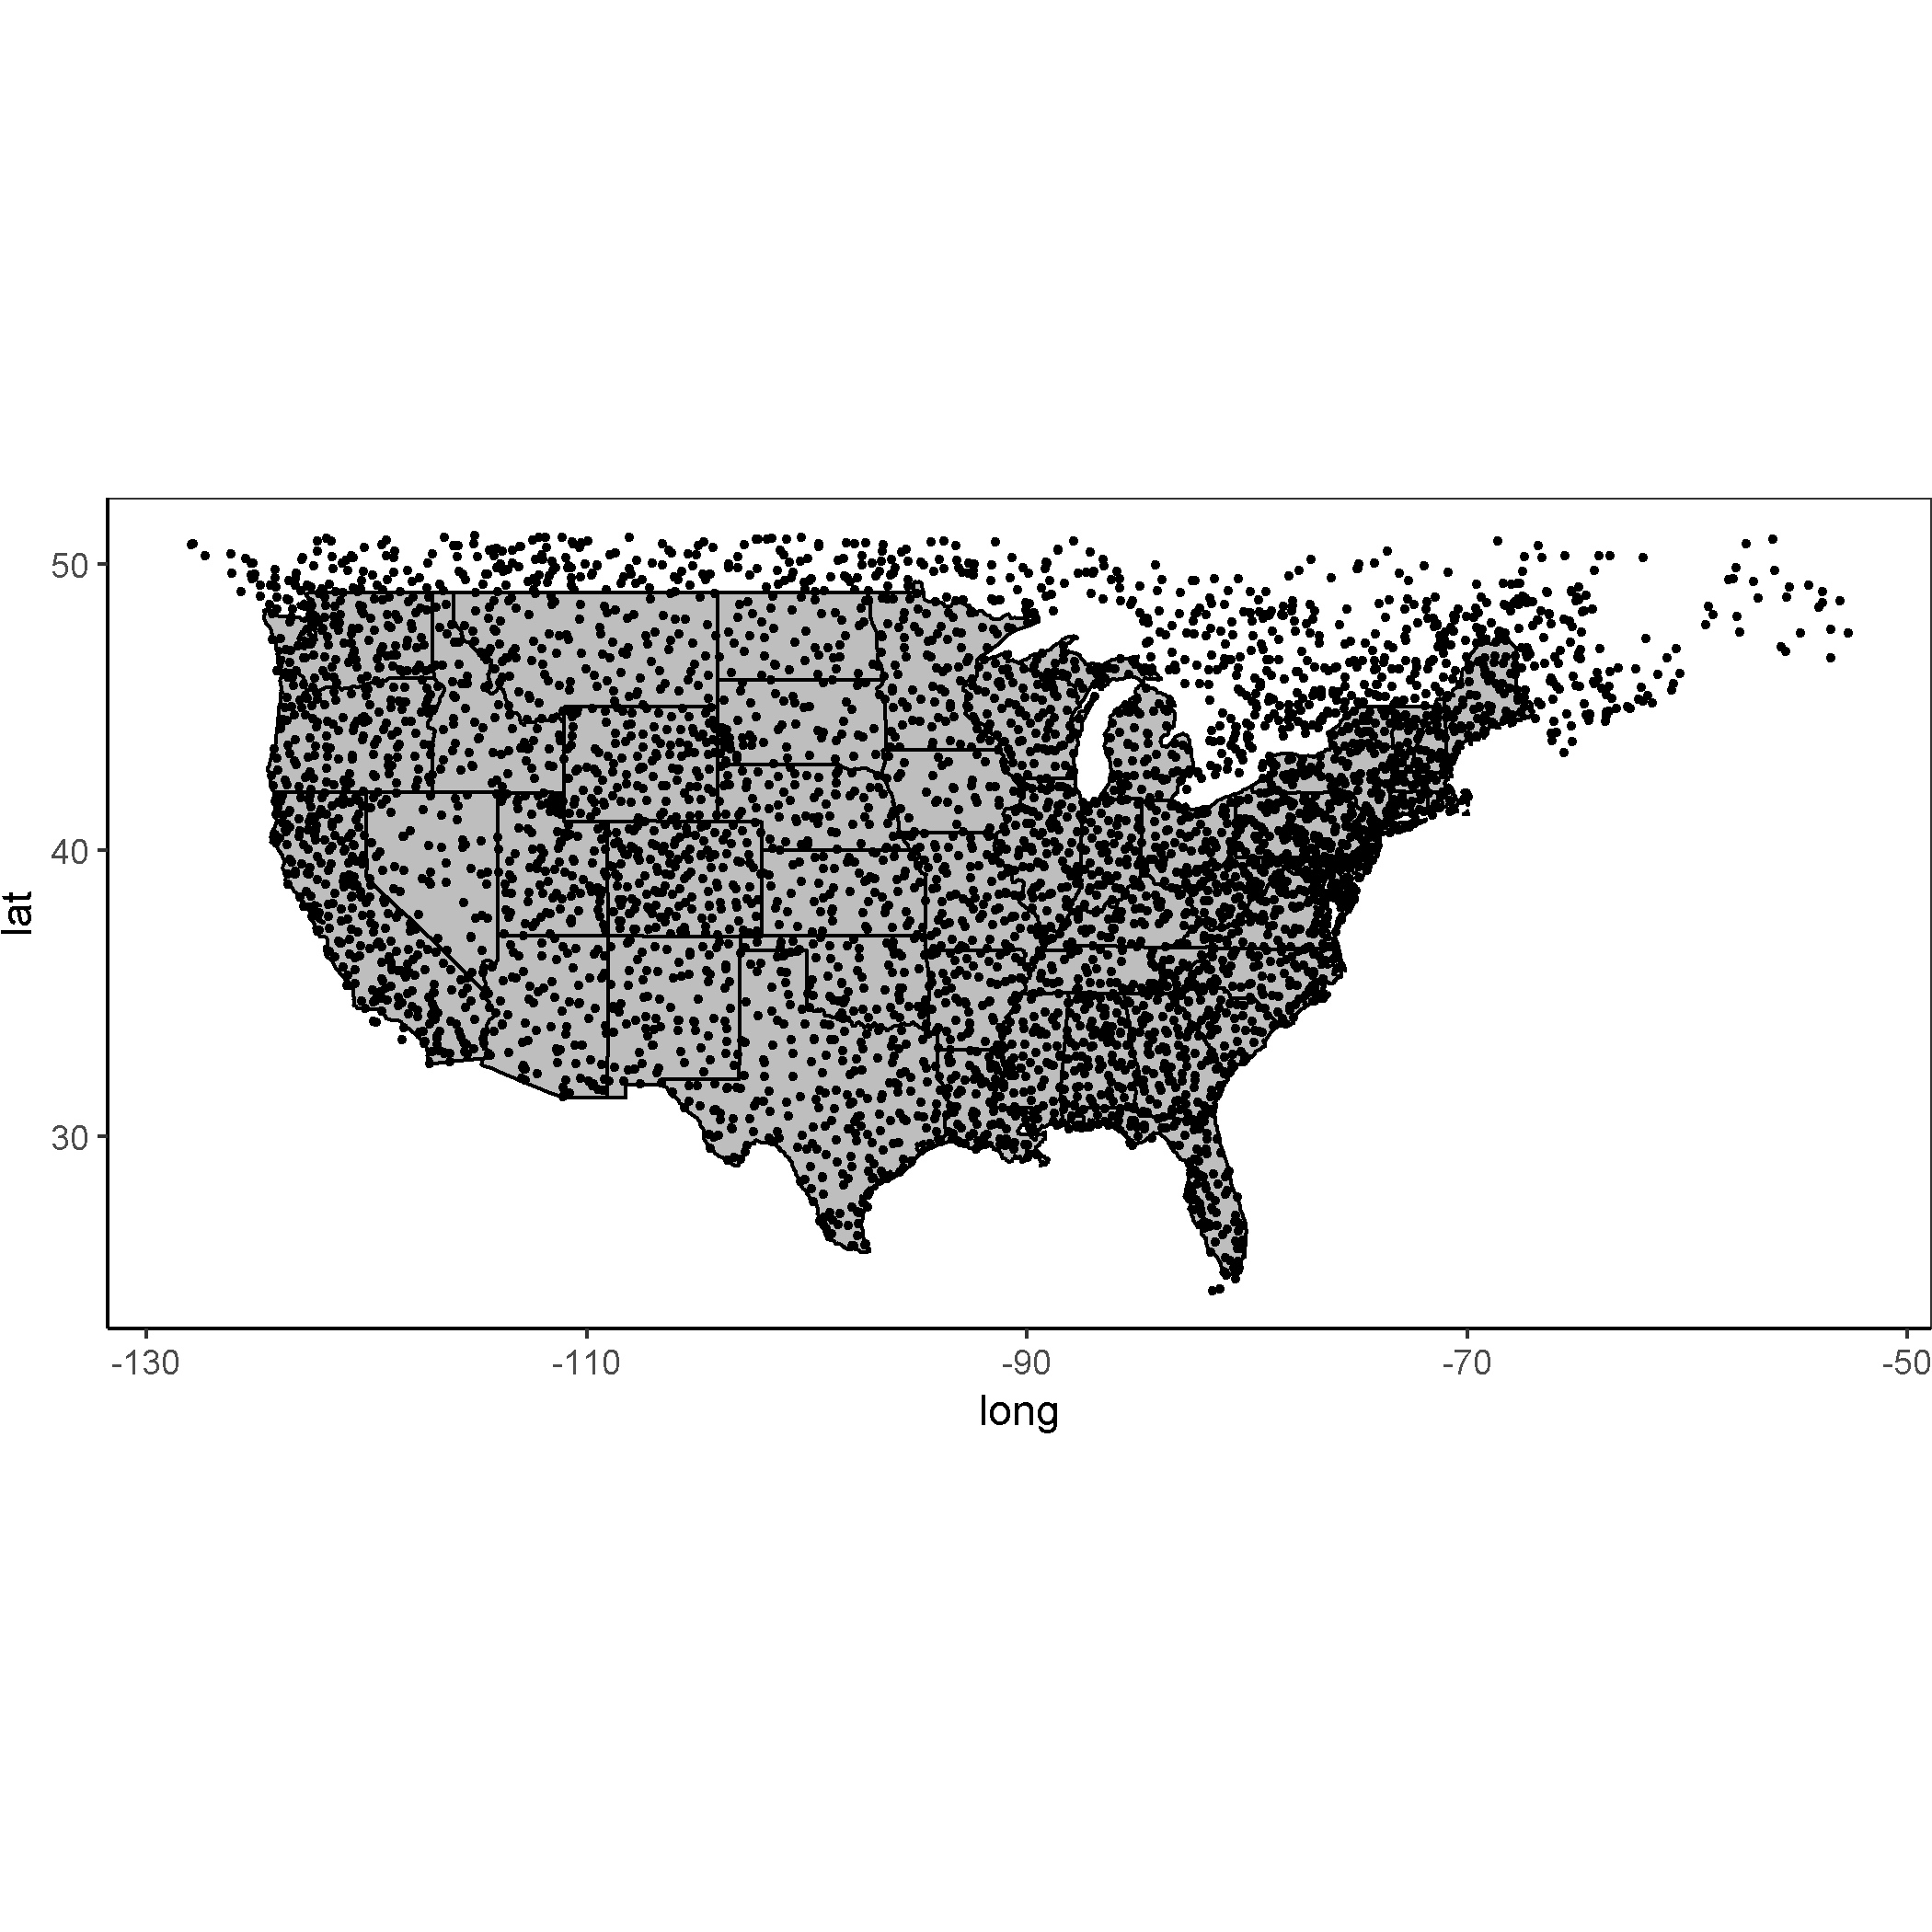
\includegraphics[width=0.85\linewidth]{./chapterFiles/fisherSpatial/figures/figsCalledInDiss/bbsRoutesUsed} 

}

\caption{Locations of Breeding Bird Survey routes sampled between 1966 and 2017.}\label{fig:bbsPoints}
\end{figure}
\hypertarget{study-area}{%
\subsection{Study area}\label{study-area}}

Although the NABBS conducts surveys throughout much of North America, I limited analyses to the continental United States and parts of southern Canada. NABBS coverage of the boreal forests of Canada are sparse in space, and many routes in Mexico have fewer than 25 years of observations.
\begin{figure}[h]

{\centering 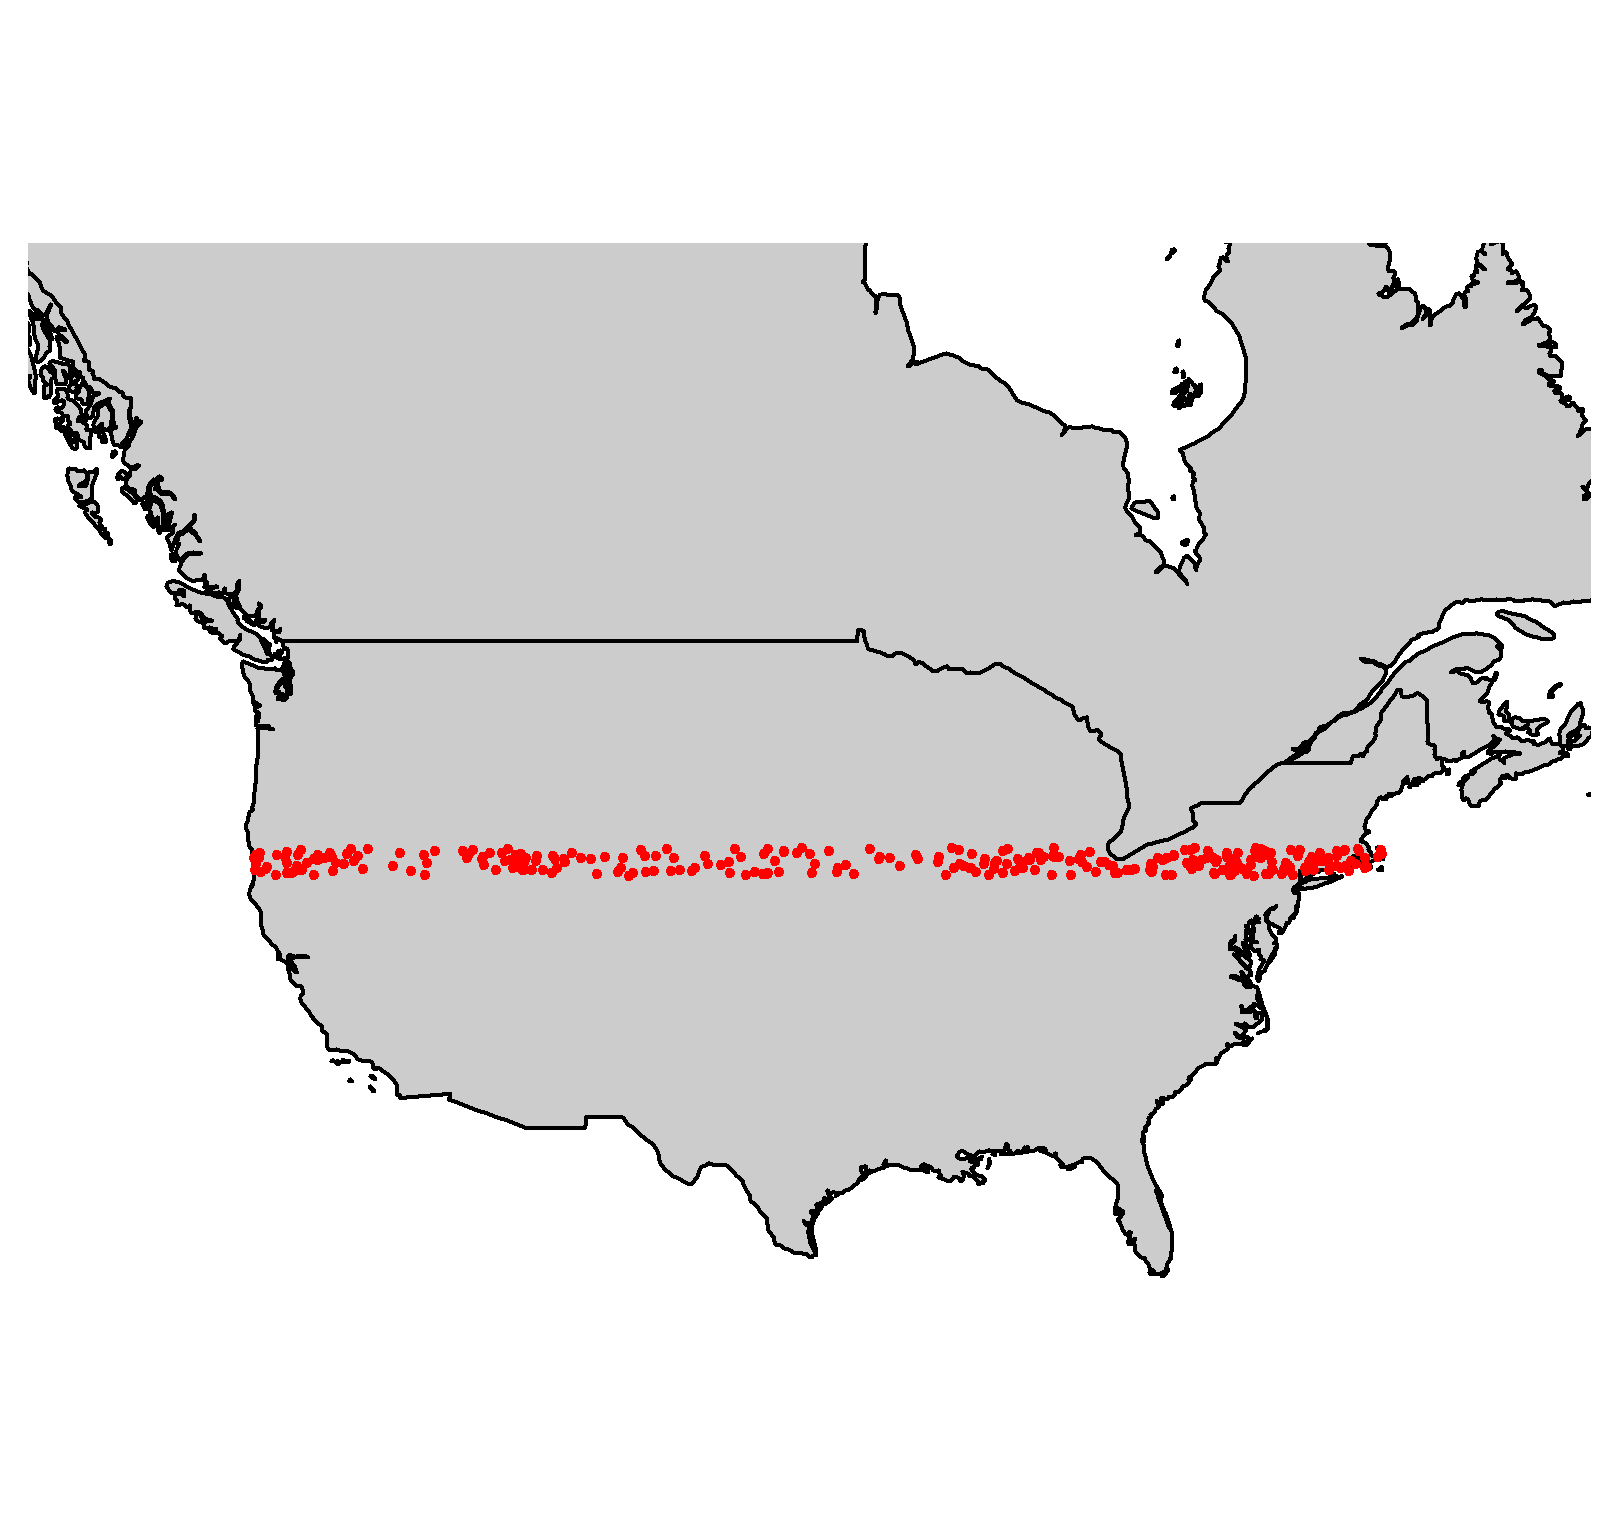
\includegraphics[width=0.85\linewidth]{./chapterFiles/fisherSpatial/figures/figsCalledInDiss/transectSamplingEx_1row} 

}

\caption{A single East-West transect of Breeding Bird Survey routes used to calculate the Fisher Information.}\label{fig:ewRouteMap}
\end{figure}
\hypertarget{focal-military-base}{%
\subsubsection{Focal military base}\label{focal-military-base}}

The Mission of the US Department of Defense is to provide military forces to deter war and protect the security of the country, and a primary objective of individual military bases is to maintain military readiness. To maintain readiness, military bases strictly monitor and manage their natural resources. Military bases vary in size and nature, and are heterogeneously distributed across the continental United States (See Fig. \ref{fig:ewRouteMap}). The spread of these bases (Fig. \ref{fig:milBases}), coupled with the top-down management of base-level natural resources presumably influences the inherent difficulties associated with collaborative management within and across military bases and other natural resource management groups (e.g., state management agencies, non-profit environmental groups.

Much like other actively managed landscapes, miltiary bases are typically surrounded by non- or improperly-managed lands. Natural resource managers of military bases face environmental pressures within and surrounding their properties, yet their primary objectives are very different. Natural resource managers of military bases, whose primary objective is to maintain military readiness, are especially concerned with if and how broad-scale external forcings might influence their lands. Prominent concerns include invasive species, wildlife disease, and federally protected species (personal communication with Department of Defense natural resource managers at Eglin Air Force and Fort Riley military bases). For these reasons, natural resource managers attempt to create buffers along their perimeters (e.g., live fire/ammunitions suppression, wide fire breaks). Identifying the proximity of military bases to historic and modern ecological shifts may provide insight into the effectiveness of their natural resource management efforts.
\begin{figure}[h]

{\centering 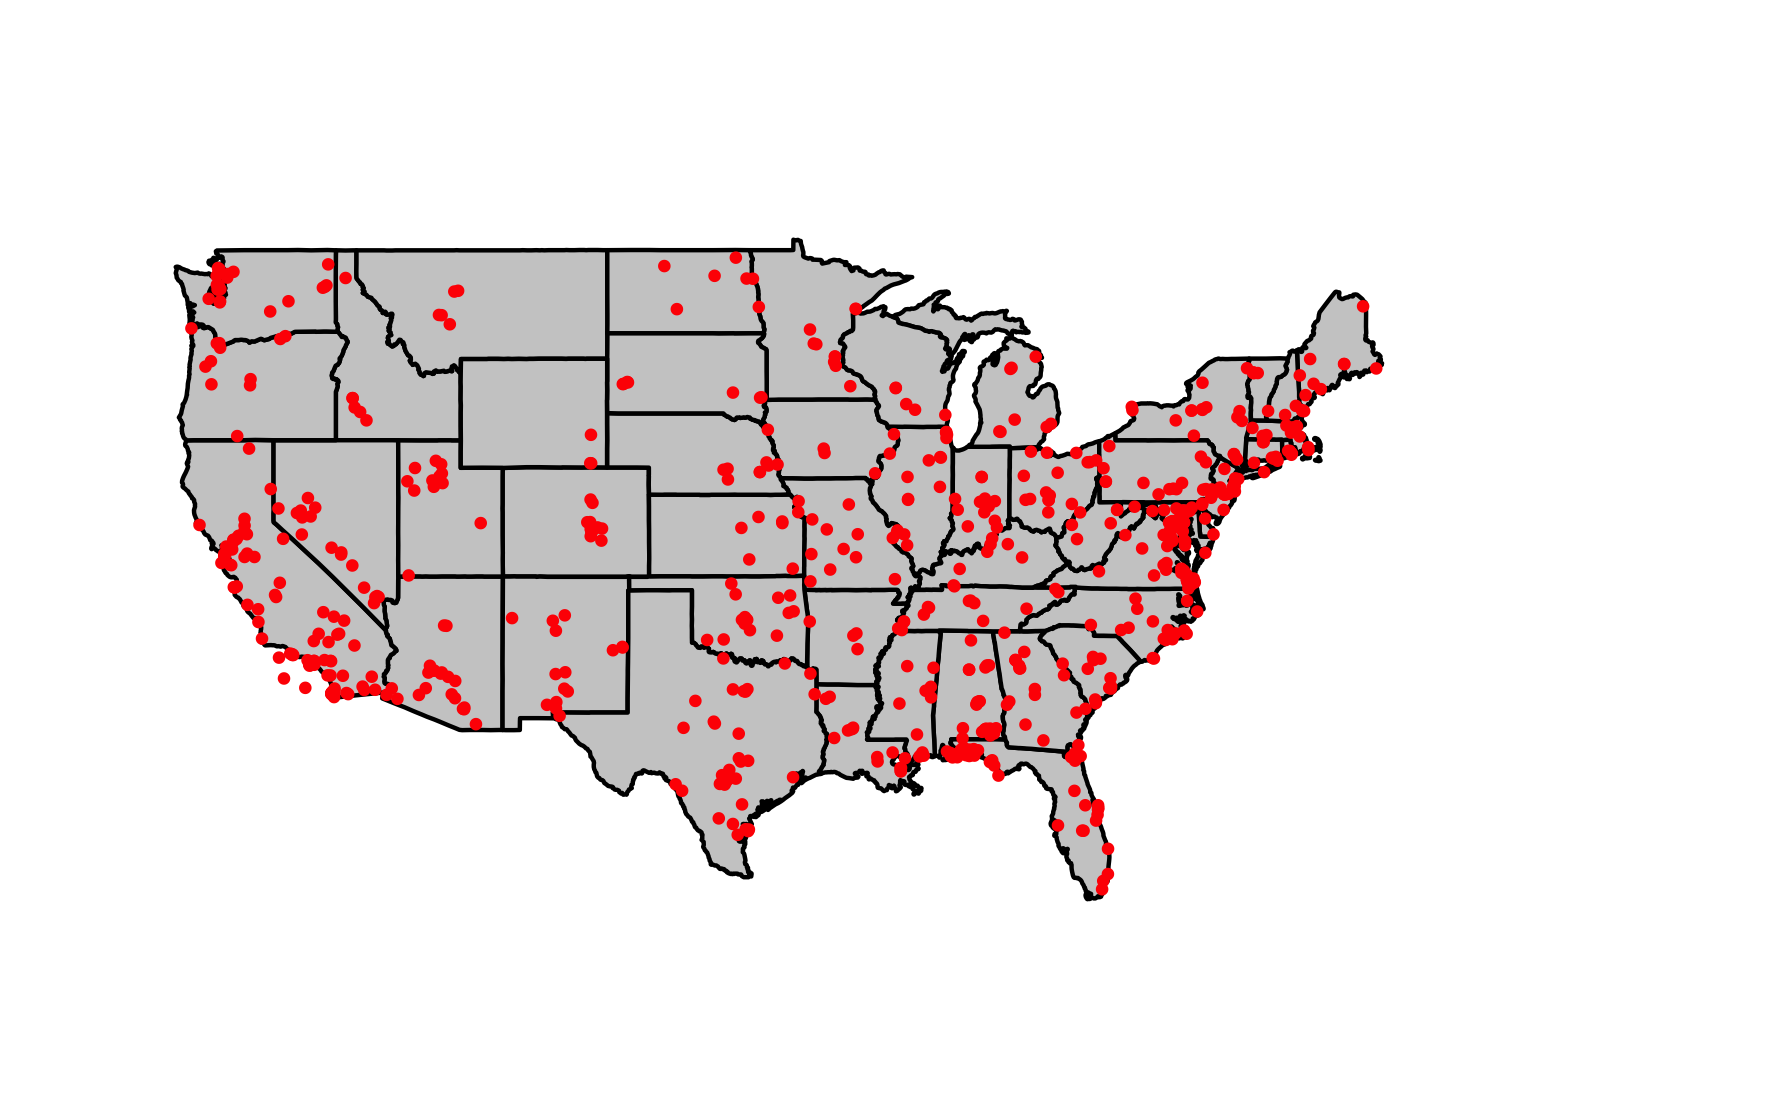
\includegraphics[width=0.85\linewidth]{./chapterFiles/fisherSpatial/figures/figsCalledInDiss/milBases} 

}

\caption{Locations of U.S. military bases in our study area.}\label{fig:milBases}
\end{figure}
The NABBS routes chosen for analyses in this Chapter lie within or near Fort Riley military base (located at approximately \(39.110474^{\circ}\), \(-96.809677^{\circ}\); Kansas, USA). Fort Riley (\ref{fig:basesOfInterestMap}) is a useful reference site for this study. Woody encroachment of the Central Great Plains over the last century has triggered shifts in dominant vegetative cover and diversity (Ratajczak et al.~2012) in the area surrounding Fort Riley military base (e.g., Van Auken 2009). This phenomena should present itself as a regime boundary should Fisher Information be a robust regime shift detection method.
\begin{figure}[h]

{\centering 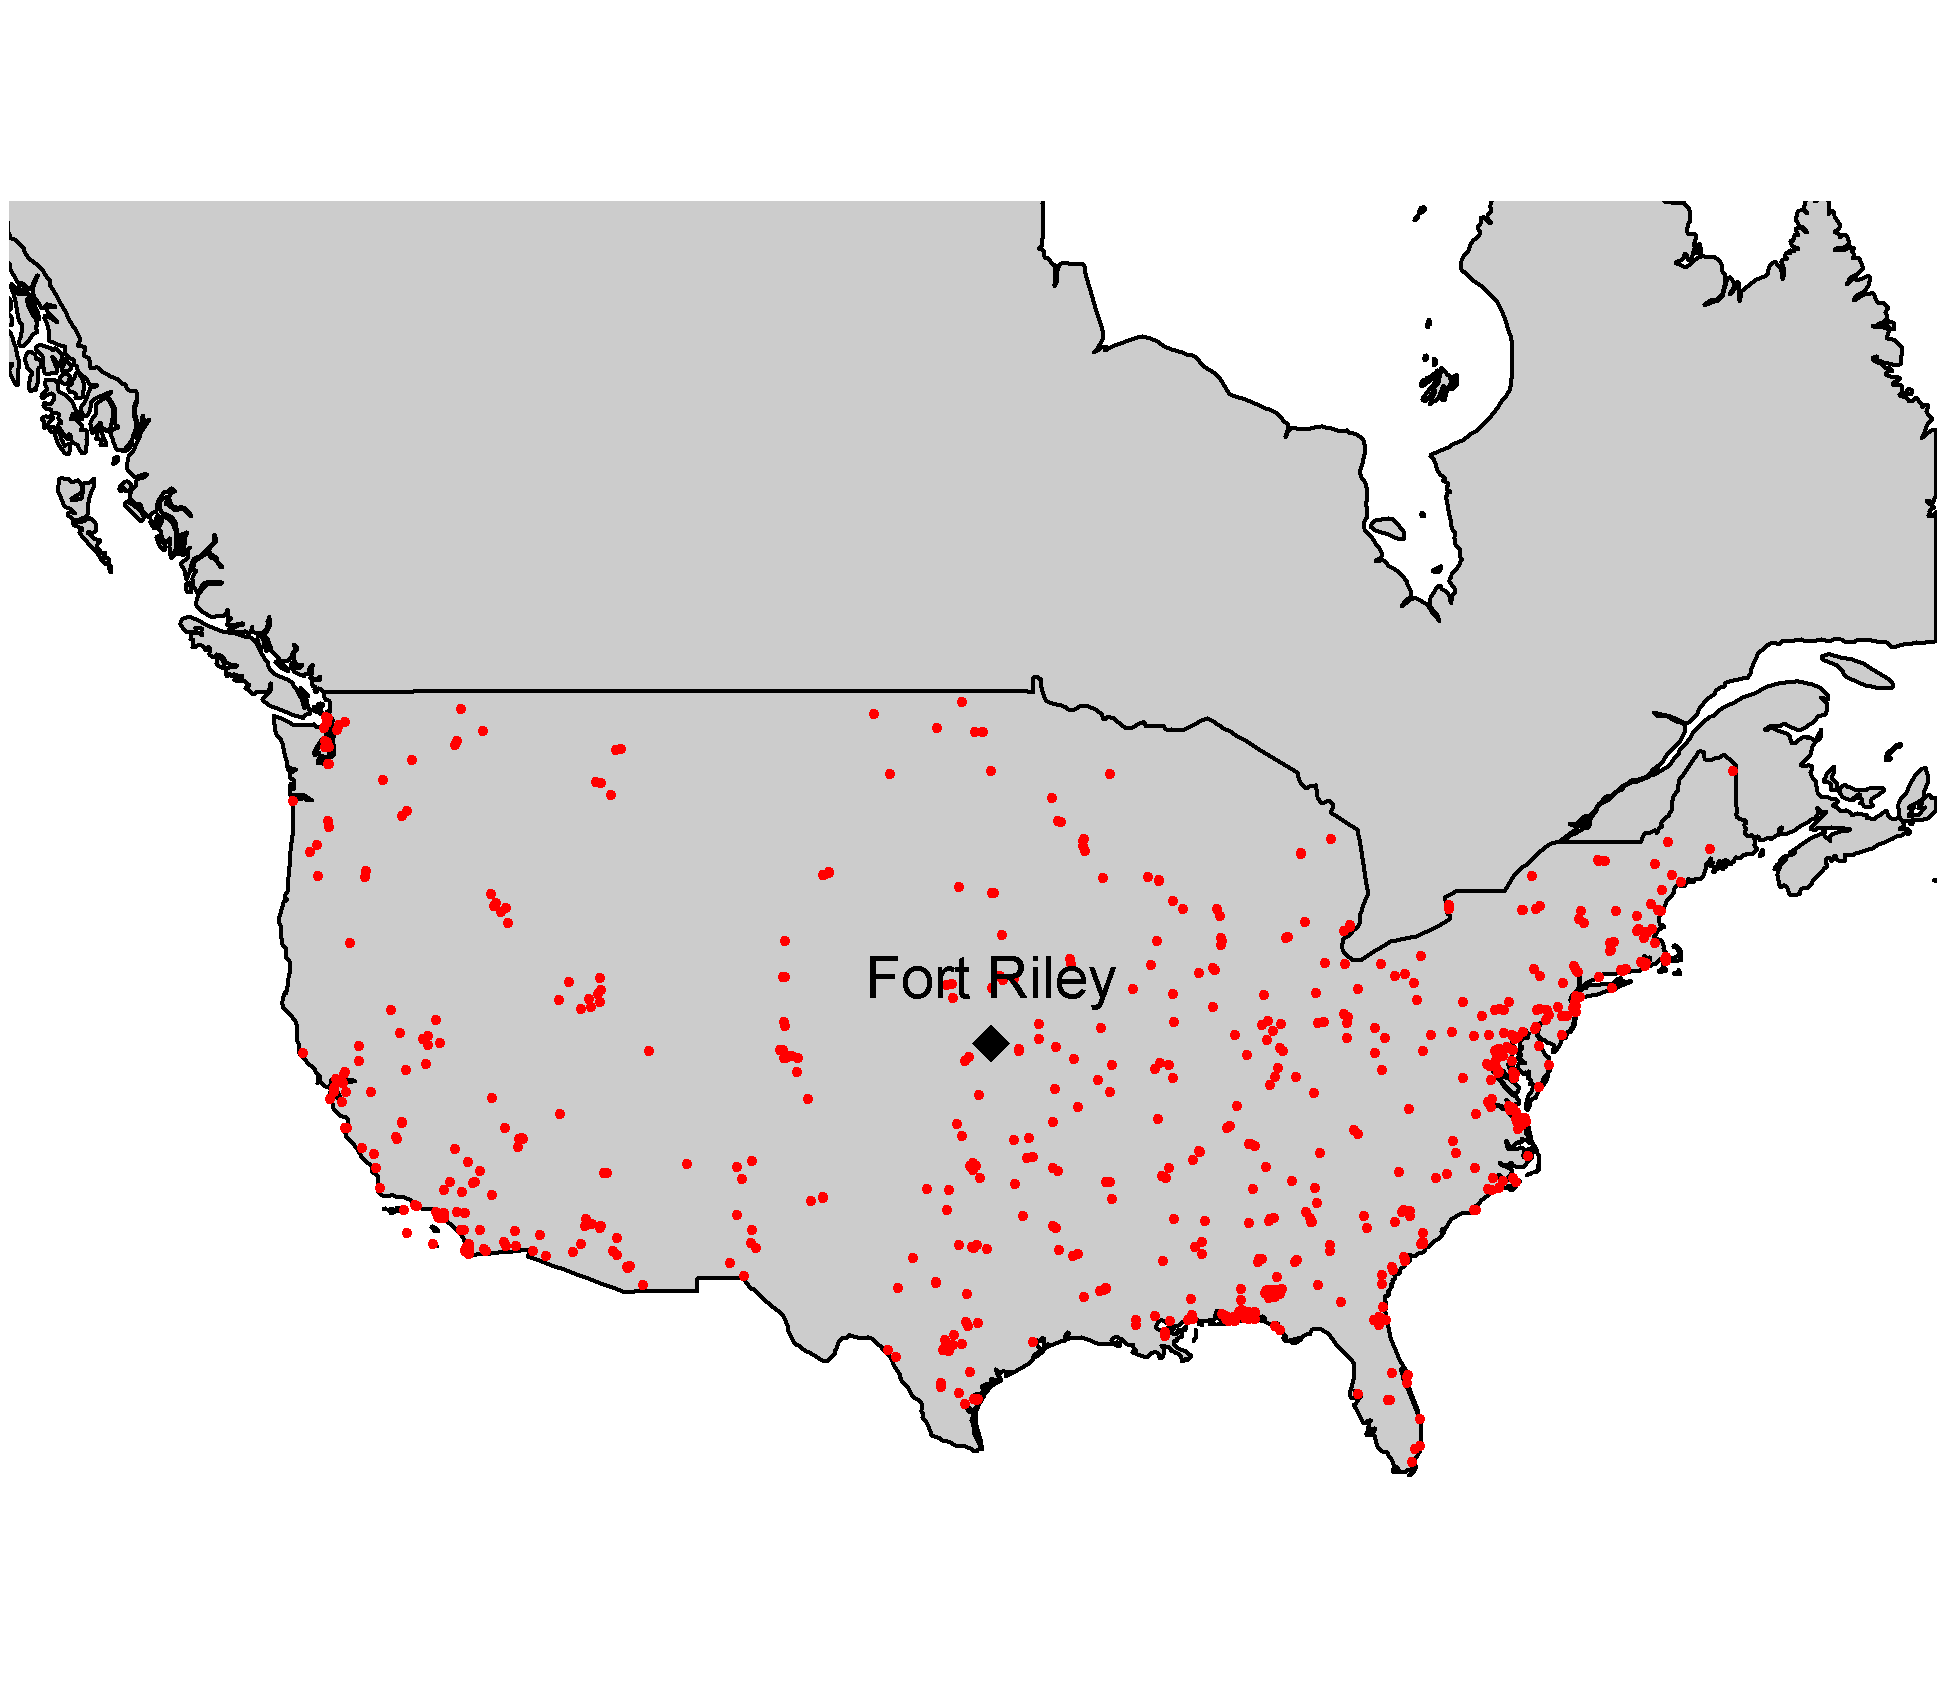
\includegraphics[width=0.85\linewidth]{./chapterFiles/fisherSpatial/figures/figsCalledInDiss/basesOfInterestMap} 

}

\caption{Locations of focal U.S. military bases, Eglin Air Force Base (AFB) and Fort Riley Military Base.}\label{fig:basesOfInterestMap}
\end{figure}
\hypertarget{spatial-sampling-grid}{%
\subsubsection{Spatial sampling grid}\label{spatial-sampling-grid}}

To my knowledge, Sundstrom, Eason, Nelson, Angeler, Barichievy, Garmestani, Graham, et al. (2017a) is the only study to use the Fisher Information on spatially-referenced data. The authors of this study hand-picked NABBS routes to be included in their samples such that their metrics should detect `regime changes' when adjacent sampling points represented different ecoregions (broad-scale vegetation classification system). The authors also suggest each ecoregion is similarly represented, having a similar number of NABBS routes within each ecoregion in the analysis. However, this method of handpicking routes resulted in a transect which was neither North-South nor East-West running (see Sundstrom, Eason, Nelson, Angeler, Barichievy, Garmestani, Graham, et al. (2017a)), but rather zigzagged across a midwestern region.
\begin{figure}[h]

{\centering \includegraphics[width=0.85\linewidth]{./chapterFiles/fisherSpatial/figures/figsCalledInDiss/transectSamplingALlRoutesUsed} 

}

\caption{The three East-West running transects used to visualize results in this chapter.}\label{fig:ewRoutesUsedHere}
\end{figure}
I constructed a gridded system across the continental United States and parts of Canada. The gridded system comprises East-West running transects transects running in either North-South or East-West directions. This method ameliorates some sampling bias, as I have arbitrarily defined sampling transects, rather than hand-picking sites to include in the analysis. Additionally, this approach allows for raster stacking, or layering data layers (e.g., vegetation, LIDAR, weather) on top of the sampling grid and results, allowing one to identify potential relationships with large-scale drivers. This method also provides a simple vector for visualizing changes in the Fisher Information over space-time, using animations and still figures. For brevity, I present visual results of only three, spatially-adjacent, East-West running transects (Fig. \ref{fig:ewRoutesUsedHere}) at multiple time periods.

\hypertarget{calculating-fisher-information-fi}{%
\subsection{Calculating Fisher Information (FI)}\label{calculating-fisher-information-fi}}

Fisher Information, \(I(\theta)\), was developed in 1922 by Ronald Fisher as a measure of the amount of information that an observable variable, X, reveals about an unknown parameter, \(\theta\). Fisher Information is a measure of indeterminacy (Fisher 1922) and is defined as,
\begin{equation} 
  I(\theta) = \int \frac{dy}{p(y|\theta)}\left[\frac{dp(y|\theta)}{d\theta}\right]^2
  \label{eq:fiGeneral1922}
\end{equation}
where \(p(y|\theta)\) is the probability density of obtaining the data in presence of \(\theta\). The Fisher Information measure (FIM) is used to calculate the covariance matrix associated with the likelihood, \(p(y|\theta)\). Fisher Information is described as Extreme Physical Information (EPI; Frieden and Soffer 1995, Kibble 1999, Frieden et al.~2002), a measure that has been used to track the complexity of systems in many scientific disciplines including, physics, cancer research, electrical engineering, and, recently, complex systems theory and ecology

Fisher Information as gathered from observational data provides insight as to the dynamic order of a system, where an orderly system is one with constant (i.e., unchanging) observation points, and one whose nature is highly predictable. A disorderly system is just the opposite, where each next data point is statistically unpredictable. In ecological systems, patterns are assumed to be a realization of ecosystem order; therefore, oneshould expect orderliness in a system with relatively stable processes and feedbacks. Orderliness, however, does not necessarily infer long-term predictability. \eqref{eq:fiGeneral1922} is next adapted to estimate the dynamic order of an entire system, \(s\), as
\begin{equation} 
  I = \int \frac{ds}{p(s)}\left[\frac{dp(s)}{ds}\right]^2
\end{equation}
where \(p(s)\) is the probability density for \(s\). Here, a relatively high Fisher Information value (\(I\)) infers higher dynamic order, whereas a lower value (approaching zero) infers less orderliness. To limit the potential values of \(I\) in real data, we can calculate the amount of Fisher Information by re-expressing it in terms of a probability amplitude function \(q(s)\) (Fath et al.~2003, Mayer et al.~2007, eq. 7.3):
\begin{equation}
  I = 4 \int ds\left[\frac{dq(s)}{ds}\right]^2
  \label{eq:fiAmp}
\end{equation}
A form specific to the pdf of distance travelled by the entire system, which I call the `derivatives' method, is defined as (Mayer et al., 2007, eq. 7.12):
\begin{equation}
  I = \frac{1}{T} \int_0^T dt\left[\frac{s''^2}{s'^4}\right]^2
  \label{eq:fiDerivs}
\end{equation}
where T is the number of equally spaced time points over which the data are integrated. Numerical calculation of \(I\) using the binning method (Eq. \eqref{eq:fiAmp} and \eqref{eq:derivativesFI}) each incorporate a moving-window procedure for calculating the probability of the system, \(p(s)\), as being in one of an unidentified number of states (\(s\)). Although previously applied to spatially-explicit terrestrial community data,the binning method (Eq. \ref{derivatives}) requires multiple parameters to be defined \emph{a priori}, which have been shown to influence inference based on the metric. I therefore calculated FI using the derivatives equation (Eq. \ref{fiDerivs}).

The binning procedure allows for a single point in time or space to be categorized into more than one state, which violating the properties of alternative stable states theory. The size of states (see Eason and Cabezas 2012) measure is required to construct p(s). In the case of high dimensional data, a univariate binning procedure of p(s) is not intuitive (i.e., reducing a multivariable system to a single probability distribution rather than constructing a multivariate probability distribution). Importantly, when using community or abundance data, rare or highly abundant species can influence the size of states criterion, thus influencing the assignment of each point into states. Finally, Eq. \eqref{eq:fiAmp} assumes equal spacing (in space or time) between sampling points. Each of these violations can be avoided by using Eq. \eqref{eq:fiDerivs}; Cabezas and Fath 2002, Fath et al.~2003) to calculate the Fisher Information measure. The derivatives method (Eq. \eqref{eq:fiDerivs}) estimates the trajectory of the system's state by calculating the integral of the ratio of the system's acceleration and speed in state space (Fath et al., 2003). I calculated Fisher Information using Equation \eqref{eq:fiDerivs} for all East-West transect (see Fig. \ref{fig:ewRoutesUsed}) for years 1980, 1990, 2000, and 2010.

\hypertarget{interpreting-and-comparing-fisher-information-across-spatial-transects}{%
\subsection{Interpreting and comparing Fisher Information across spatial transects}\label{interpreting-and-comparing-fisher-information-across-spatial-transects}}

\hypertarget{interpreting-fi-values}{%
\subsubsection{Interpreting FI values}\label{interpreting-fi-values}}

Here I define a potential regime change as a point(s) having a non-zero derivative, and at which relatively large changes (sharp increase or decrease) in the Fisher Information measure occur. Regime shifts are identified as data changing from one state to another, thus, rapid shifts in the value of FI should indicate the points, in time or space, at which the system undergoes reorganization. Spatial and temporal Fisher Information calculation does not vary, but interpretation of either differ in that a spatial analysis will identify a spatial regime boundary (Sundstrom, Eason, Nelson, Angeler, Barichievy, Garmestani, Graham, et al., 2017a) in space within a single time period, whereas analysis of temporal data will identify a point(s) in time at which a system in a specific location undergoes a regime shift. I follow the methods outlined in the relevant literature for interpreting the Fisher Information (e.g., Karunanithi et al., 2008, p. @eason\_evaluating\_2012).

Increases in FI is proposed as an indicator of system orderliness, where periods of relatively high values of FI indicate the system is in an ``orderly'' state, or is fluctuating around a single attractor. A rapid change in FI is supposed to indicated the system is no longer orderly and may be undergoing a reorganization phase. Whether Fisher Information can identify a switch among basins of attraction within a single, stable state (or around a single attractor) remains unknown, as does the number of states which a system can occupy. When a system occurs within any number of states equally, i.e., p(s) is equal for each state, both the derivative, (\(\frac{dq(s)}{ds}\), and \(I\) are zero. As \((\frac{dq(s)}{ds} \rightarrow \infty)\), we infer the system is approaching a stable state, and as \(\frac{dq(s)}{ds} \rightarrow 0\) the system is showing no preference for a single stable state and is on an unpredictable trajectory. \eqref{eq:fiAmp} bounds the potential values of Fisher Information at \([0, 8]\), whereas \eqref{eq:fiGeneral1922}, \eqref{eq:fi73c}, and \eqref{eq:derivativesFI} have are positively unbounded \([0, \infty)\). If the Fisher Information is assumed to represent the probability of the system being observed in some state, \(s\), then the absolute value of the Fisher Information index is relative within a single datum (here, transect). It follows that Fisher Information should be interpreted relatively, but not absolutely.

\hypertarget{interpolating-results-across-spatial-transects}{%
\subsubsection{Interpolating results across spatial transects}\label{interpolating-results-across-spatial-transects}}

Because the BBS routes are not regularly spaced, pairwise correlations of adjacent transects are not possible without either binning the Fisher Information calculations using a moving-window analysis, or interpolating the results to regularly-spaced positions in space. To avoid potential biases associated with the former option, I linearally interpolated Fisher Information within each spatial transect (Fig. \ref{fig:ewRoutesUsedHere}) at 50 points along the longitudinal axis. The 50 longitudinal points at which I interpolated were the same across each spatial transect. I used the function \emph{stats::approx()} to linearly approximate the Fisher Information. I did not interpolate values beyond the longitudinal range of the original data (using argument \emph{rule=1} in package \emph{approx}).
\begin{figure}[h]

{\centering 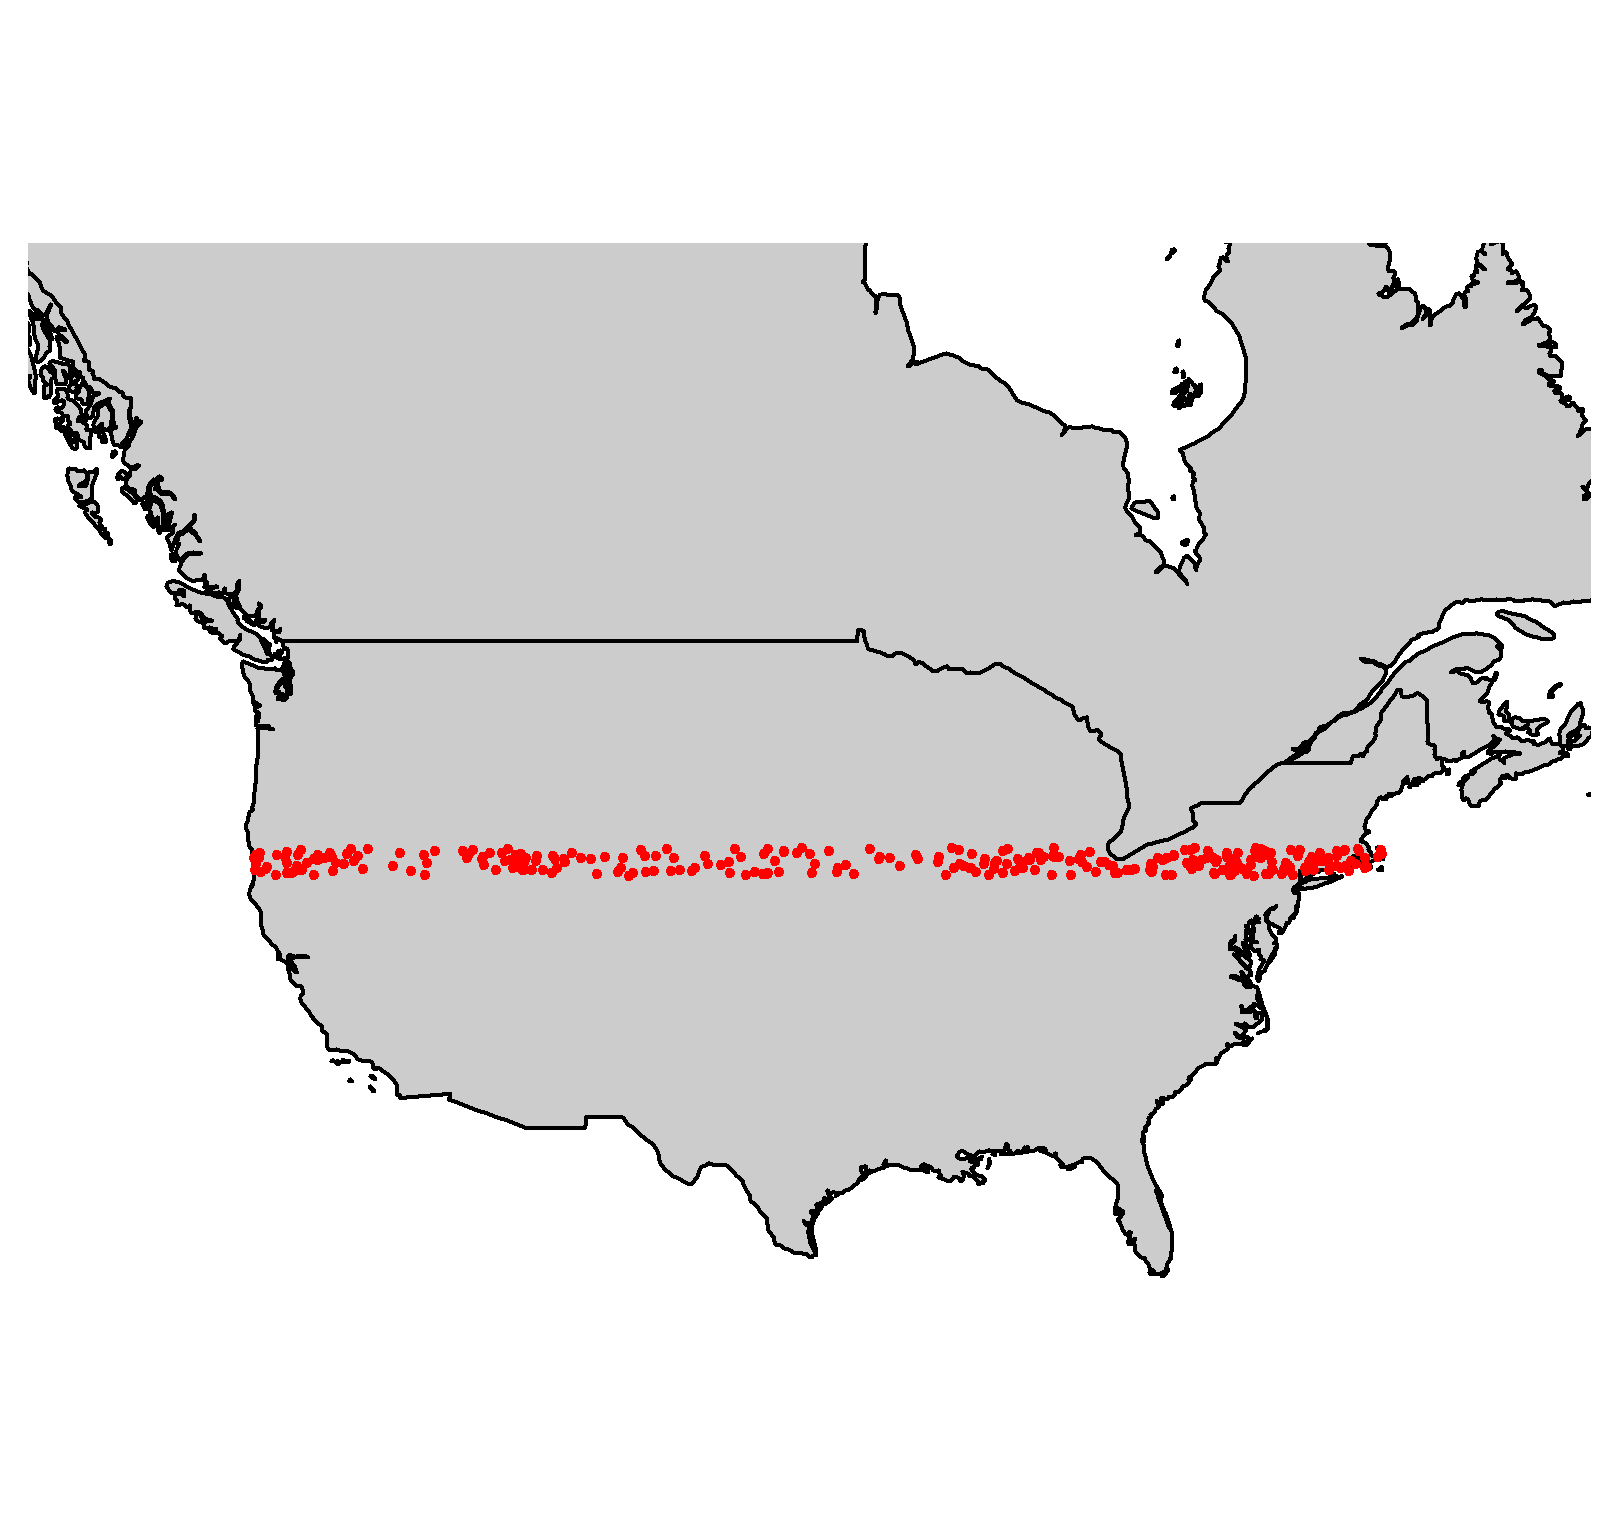
\includegraphics[width=0.85\linewidth]{./chapterFiles/fisherSpatial/figures/figsCalledInDiss/transectSamplingEx_1row} 

}

\caption{An example of two adjacent spatial transects within my sampling grid.}\label{fig:oneTsectEx}
\end{figure}
\hypertarget{spatial-correlation-of-fisher-information}{%
\subsubsection{Spatial correlation of Fisher Information}\label{spatial-correlation-of-fisher-information}}

If Fisher Information captures and reduces information regarding abrupt changes in community structure across the landscape, then the values of FI should be spatially autocorrelated. That is, the correlation of FI values should increase as the distance between points decreases. Fisher Information values calculated using Eq. \eqref{eq:derivativesFI} are \textbf{not} relatively comparable outside of our spatial transects, because the possible values are unbounded (can take on any value between \(-\infty\) and \(%\infty
\). However, because FI is directly comparabe \textbf{within} each spatial transect (e.g., \ref{fig:oneTsectEx}), we can use use pairwise correlations among two transects (e.g., \ref{fig:oneTsectEx}) to determine whether values of FI are consistent across space. I calculate the pairwise correlation (Pearson's) among each pair of adjacent spatial transects (e.g., Fig. \ref{fig:adjacentTsectEx}) using the function \emph{stats::cor()}. I removed a pair of points if at least one point was missing an estimate for Fisher Information. This occurred when the original longitudinal range of one transect exceeded its pair's range, since I did not interpolate beyond the original longitudinal range.
\begin{figure}[h]

{\centering 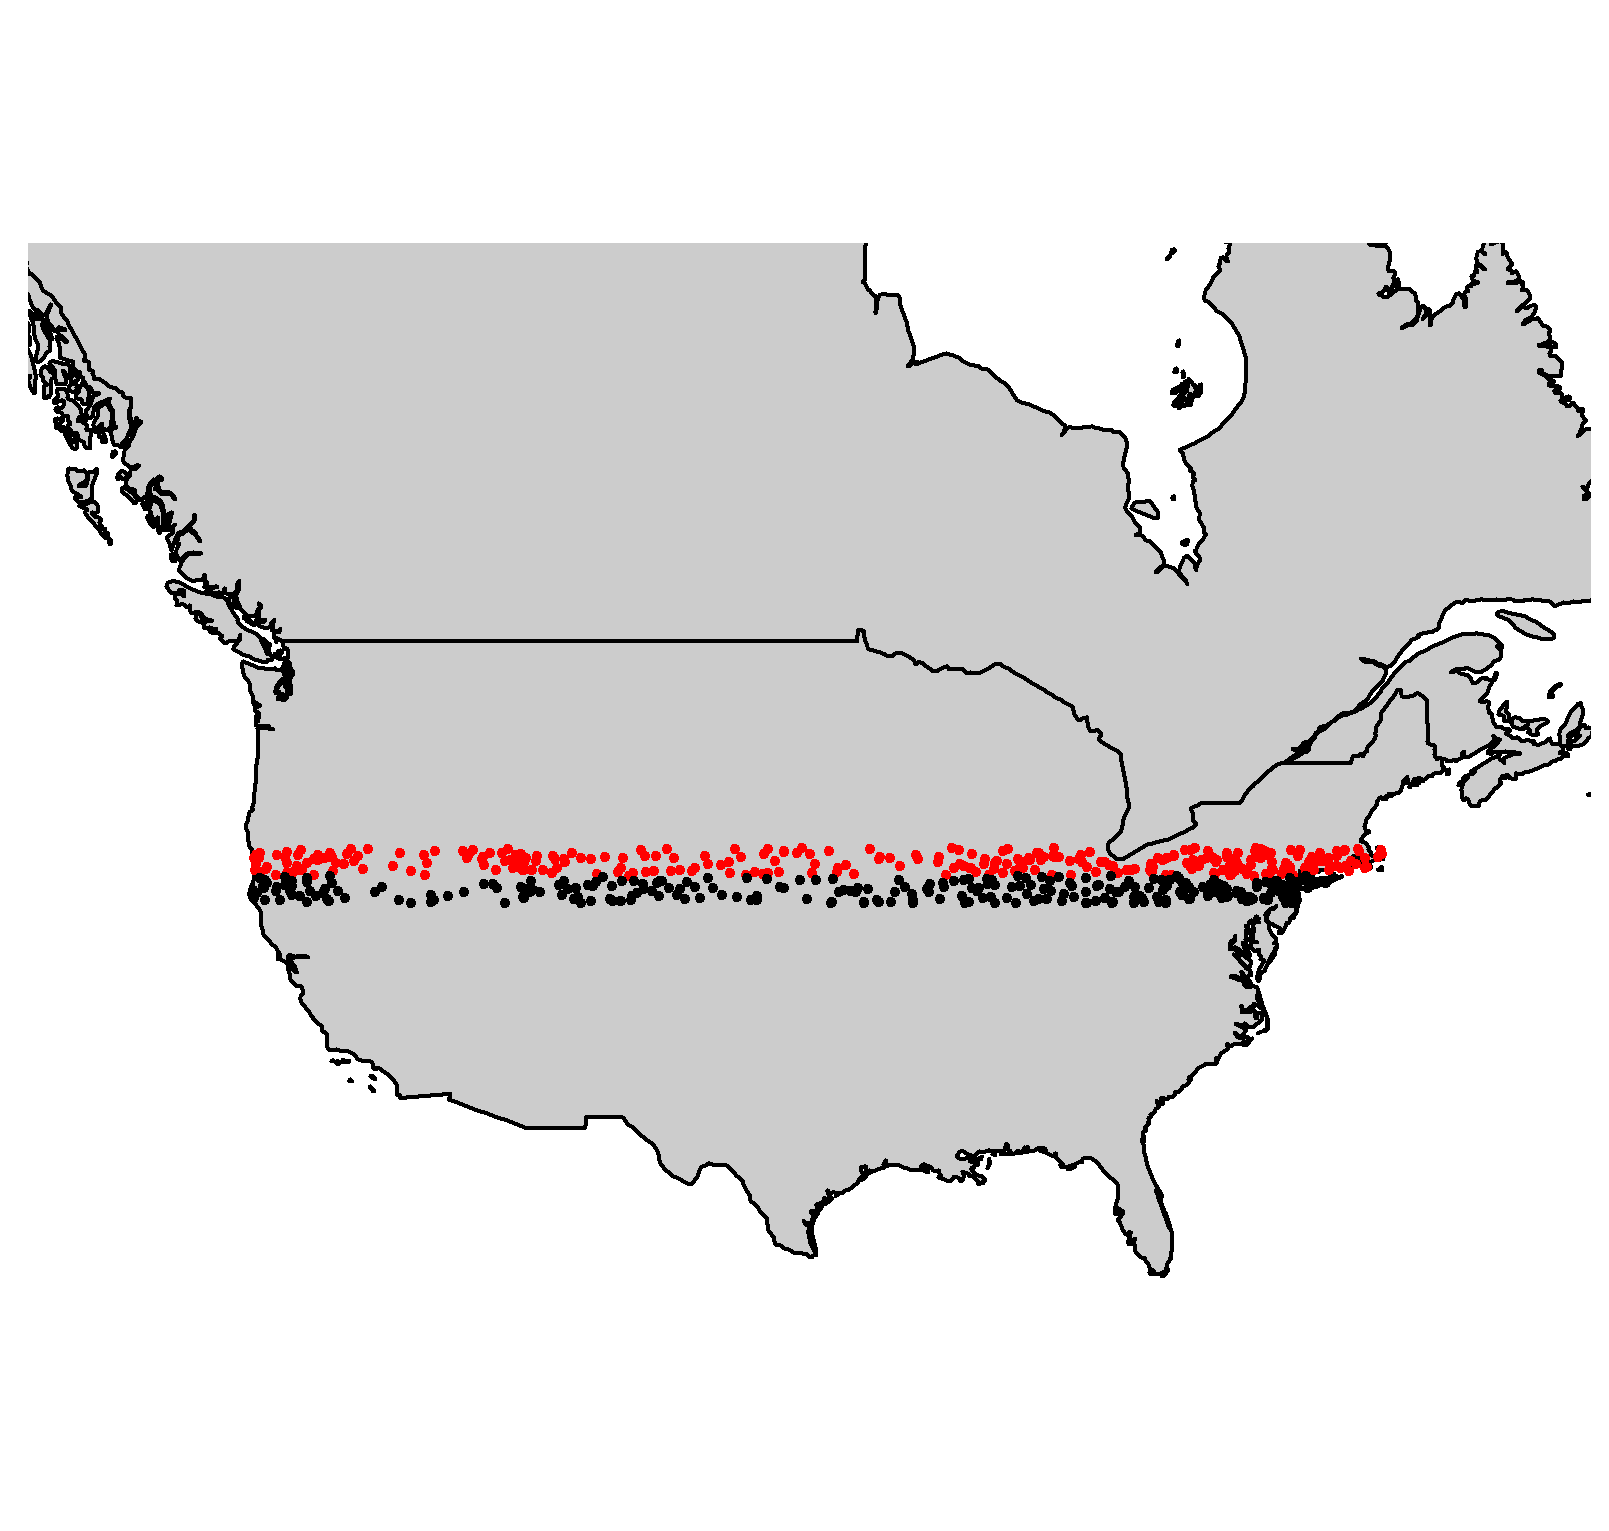
\includegraphics[width=0.85\linewidth]{./chapterFiles/fisherSpatial/figures/figsCalledInDiss/transectSamplingEx_2rows} 

}

\caption{An example of two adjacent spatial transects (12, 13) within my sampling grid.}\label{fig:adjacentTsectEx}
\end{figure}
\hypertarget{results-1}{%
\section{Results}\label{results-1}}

\hypertarget{fisher-information-across-spatial-transects}{%
\subsection{Fisher Information across spatial transects}\label{fisher-information-across-spatial-transects}}

Interpreting the Fisher Information is currently a qualitative effort. As suggested earlier, rapid increases or decreases in FI are posited indicate a change in system orderliness, potentially suggesting the location of a regime shift. Using this method yields inconclusive results regarding the location of `spatial regimes' (Fig. \ref{fig:fi1Tsect}). Of the three spatial transects analyzed in this chapter (Fig. \ref{fig:ewRoutesUsedHere}), Fig.\ref{fig:fi1Tsect} is representative of lack of pattern observed in teh Fisher Information values aross transects. I identified no clear pattern within or among spatial transects. Log-transforming the Fisher Information metric suppresses some of the extreme values, but still does not clearly identify sharp changes in the Fisher Information values.
\begin{figure}[h]

{\centering 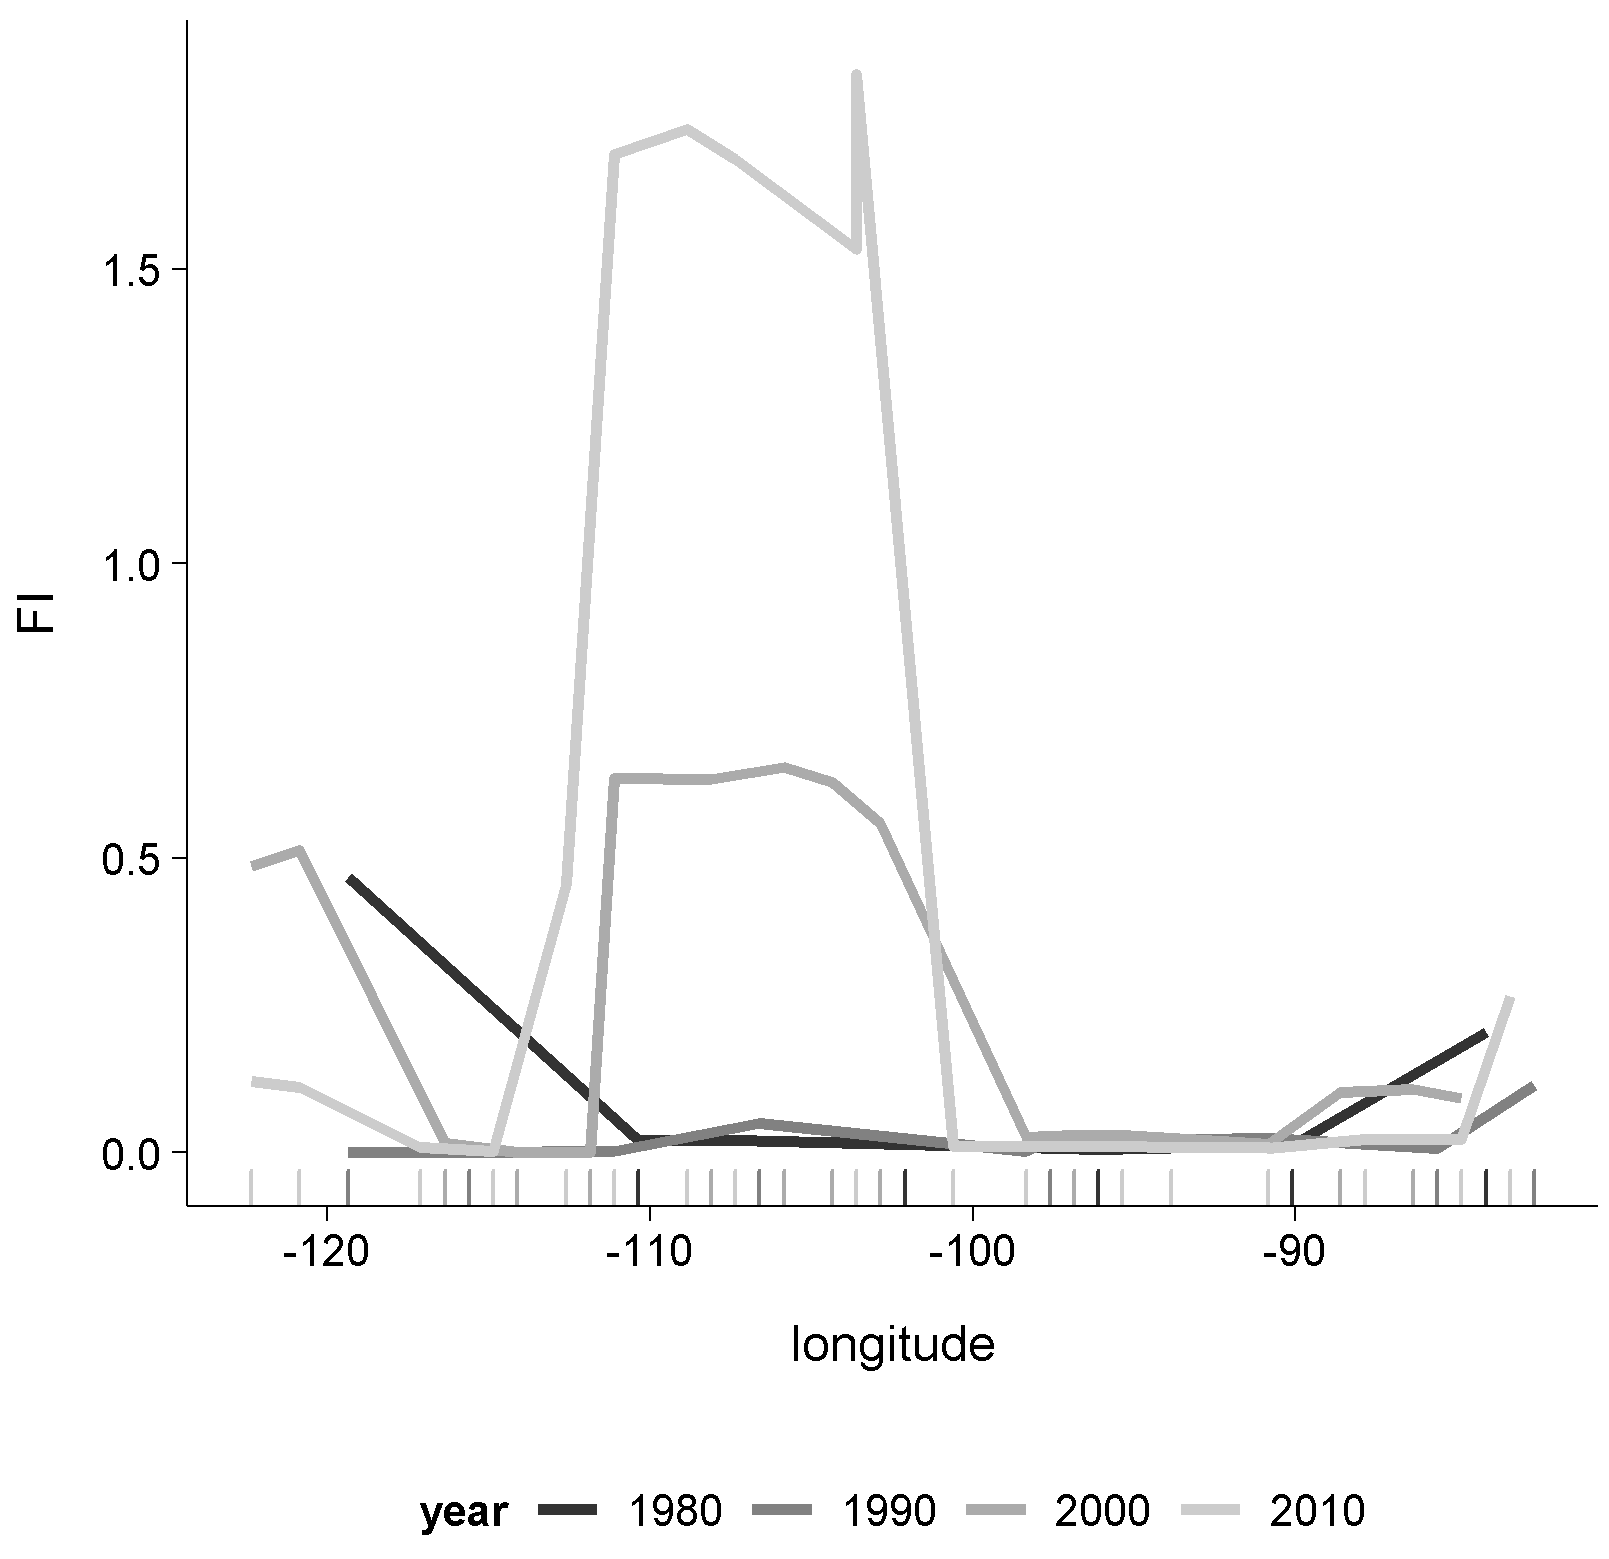
\includegraphics[width=0.85\linewidth]{./chapterFiles/fisherSpatial/figures/figsCalledInDiss/transect_12_East-West_metric_FI_Eqn7_12} 

}

\caption{Fisher Information calculated for a single transect over time.}\label{fig:fi1Tsect}
\end{figure}
\hypertarget{spatial-correlation-of-fisher-information-1}{%
\subsection{Spatial correlation of Fisher Information}\label{spatial-correlation-of-fisher-information-1}}

In addition to failing to identfiy clear geological boundaries across large swaths of our study area, (Fig \ref{fig:usaFI}) I also did not identify spatial correlation of Fisher Information among adjacent spatial transects (Fig. \ref{fig:corPlotTsectsInterp})\footnote{Pairs were compared (column) at select sampling years (rows), and pair-wise correlations among paired transects are presented. Large, positive correlations indicate Fisher Information signals similarly at adjacent spatial transects.}. For spatially-adjacent transects (e.g, transects 11 and 12, or 12 and 13 in Fig. \ref{fig:corPlotTsectsInterp}), we should expect high and positive correlation values, and these values shoudl stay consistent across time \emph{unless} the spatial transects were separated by an East-West running physical or functional boundary. This is not, however, what I expect in our East-West running transects (Fig. \ref{ewRoutesUsedHere}), as the spatial soft-boundaries limiting the distribution and functional potential of avian communities are largely North-South (Fig. @ref(ewRoutes\_ecoRegions)). Note spatial transects in Fig. @ref(fig:ewRoutes\_ecoRegions) overlap multiple, large spatial ecoregion boundaries, such that we should expect our data to identify these points (boundaries).
\begin{figure}[h]

{\centering 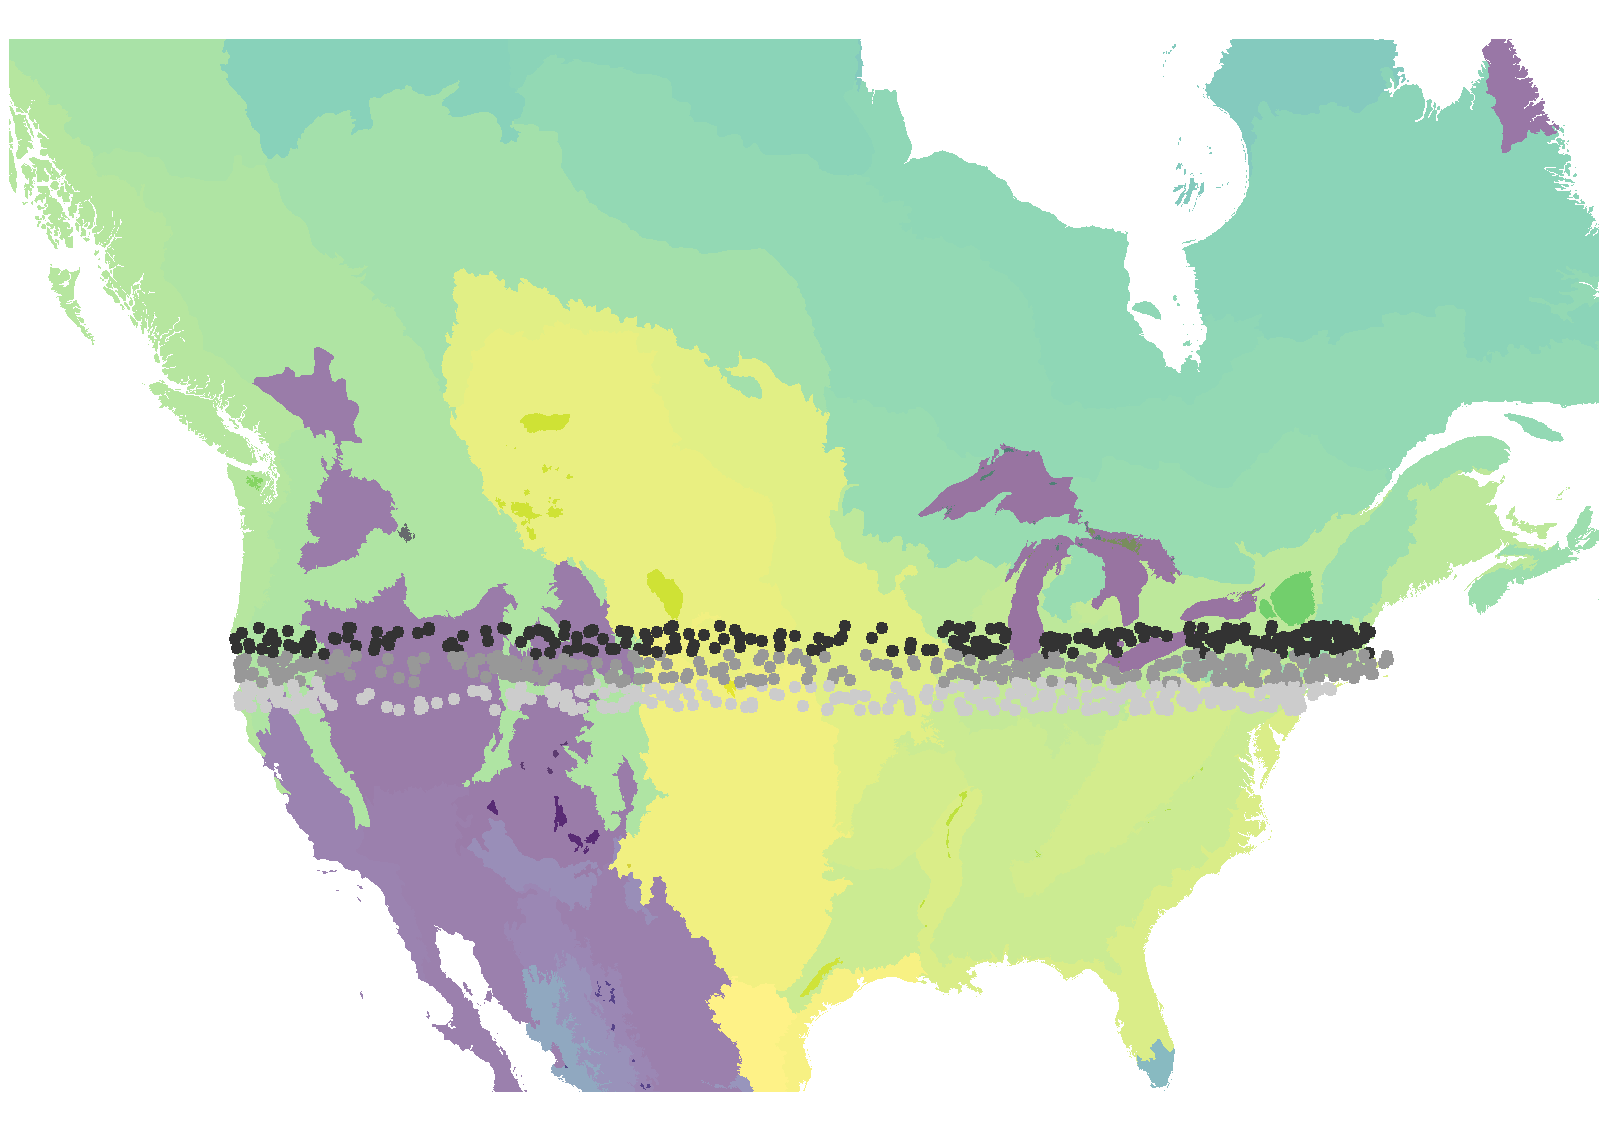
\includegraphics[width=0.75\linewidth]{./chapterFiles/fisherSpatial/figures/figsCalledInDiss/allRoutesUsed_ecoregions} 

}

\end{figure}
\begin{figure}[h]

{\centering 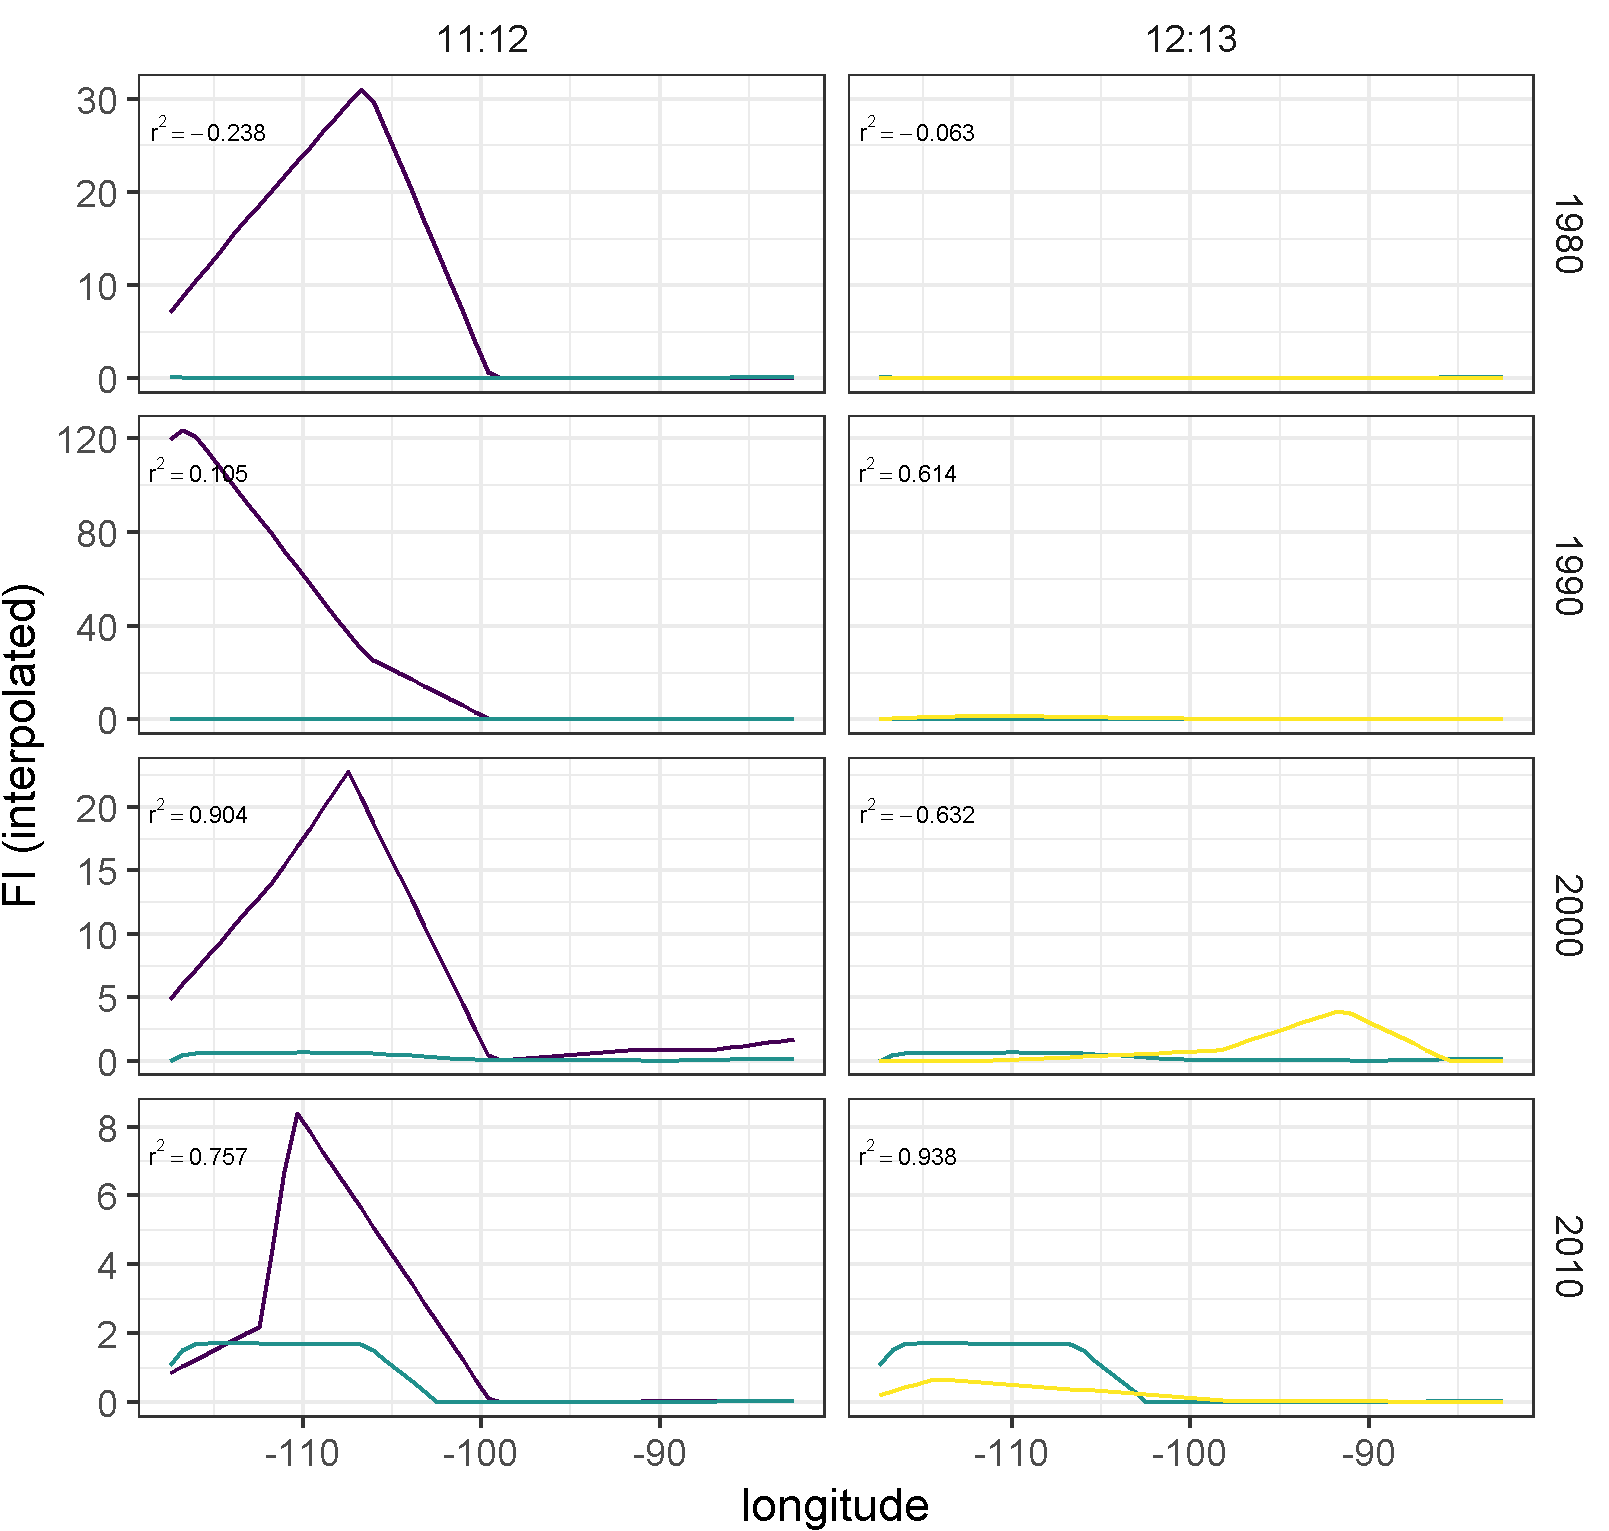
\includegraphics[width=0.85\linewidth]{./chapterFiles/fisherSpatial/figures/figsCalledInDiss/interpolated_FI_corplotSelectTransects_East-West} 

}

\caption{Pairwise relationships of Fisher Information (interpolated values) of spatially adjacent transects over time. }\label{fig:corPlotTsectsInterp}
\end{figure}
\begin{figure}[h]

{\centering 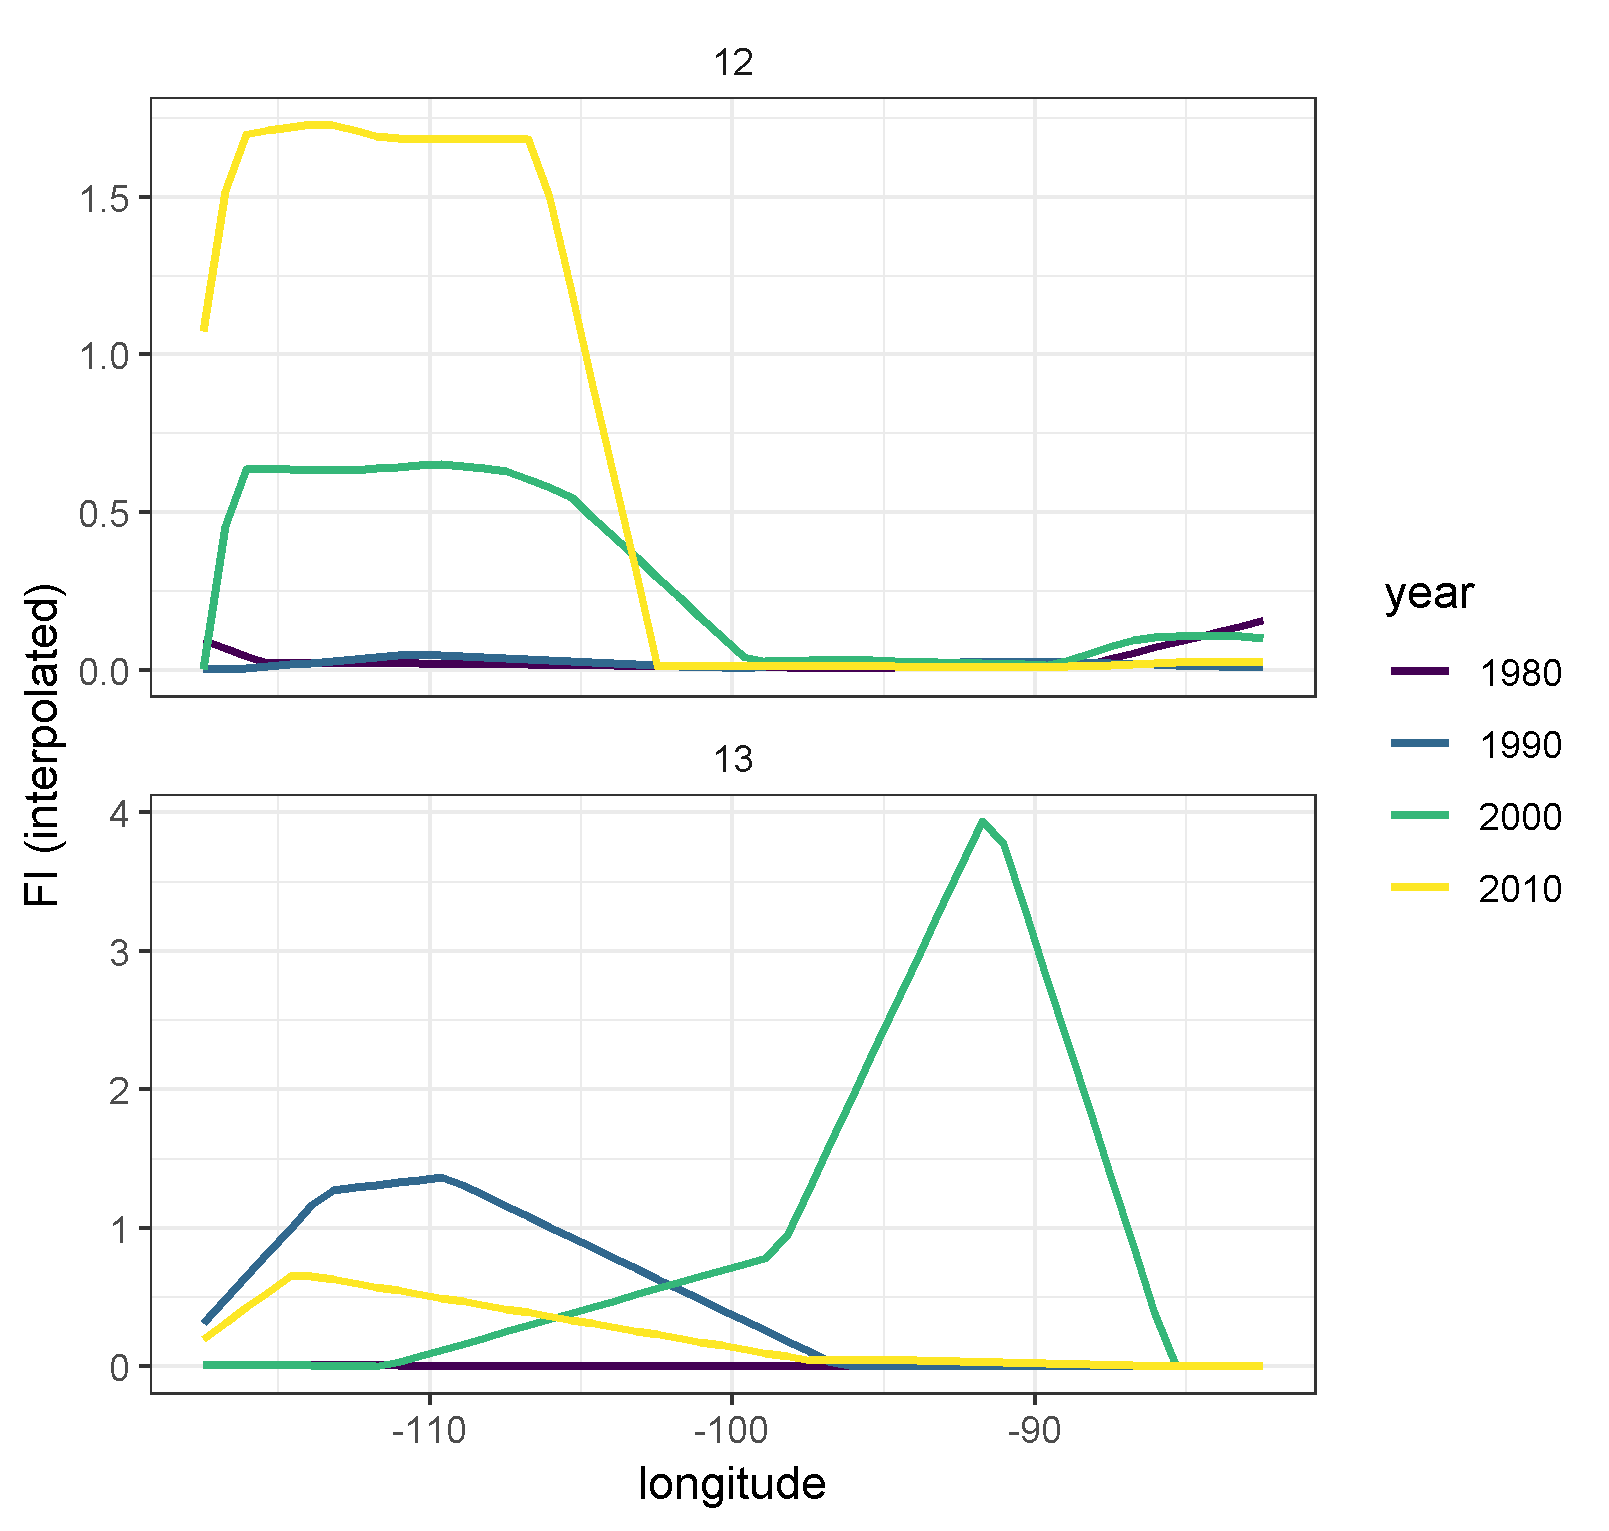
\includegraphics[width=0.85\linewidth]{./chapterFiles/fisherSpatial/figures/figsCalledInDiss/interp_FI_singlePair_corPlot_East-West} 

}

\caption{Fisher Information of two transect pairs over time. }\label{fig:fiSinglePair}
\end{figure}
\begin{figure}[h]

{\centering 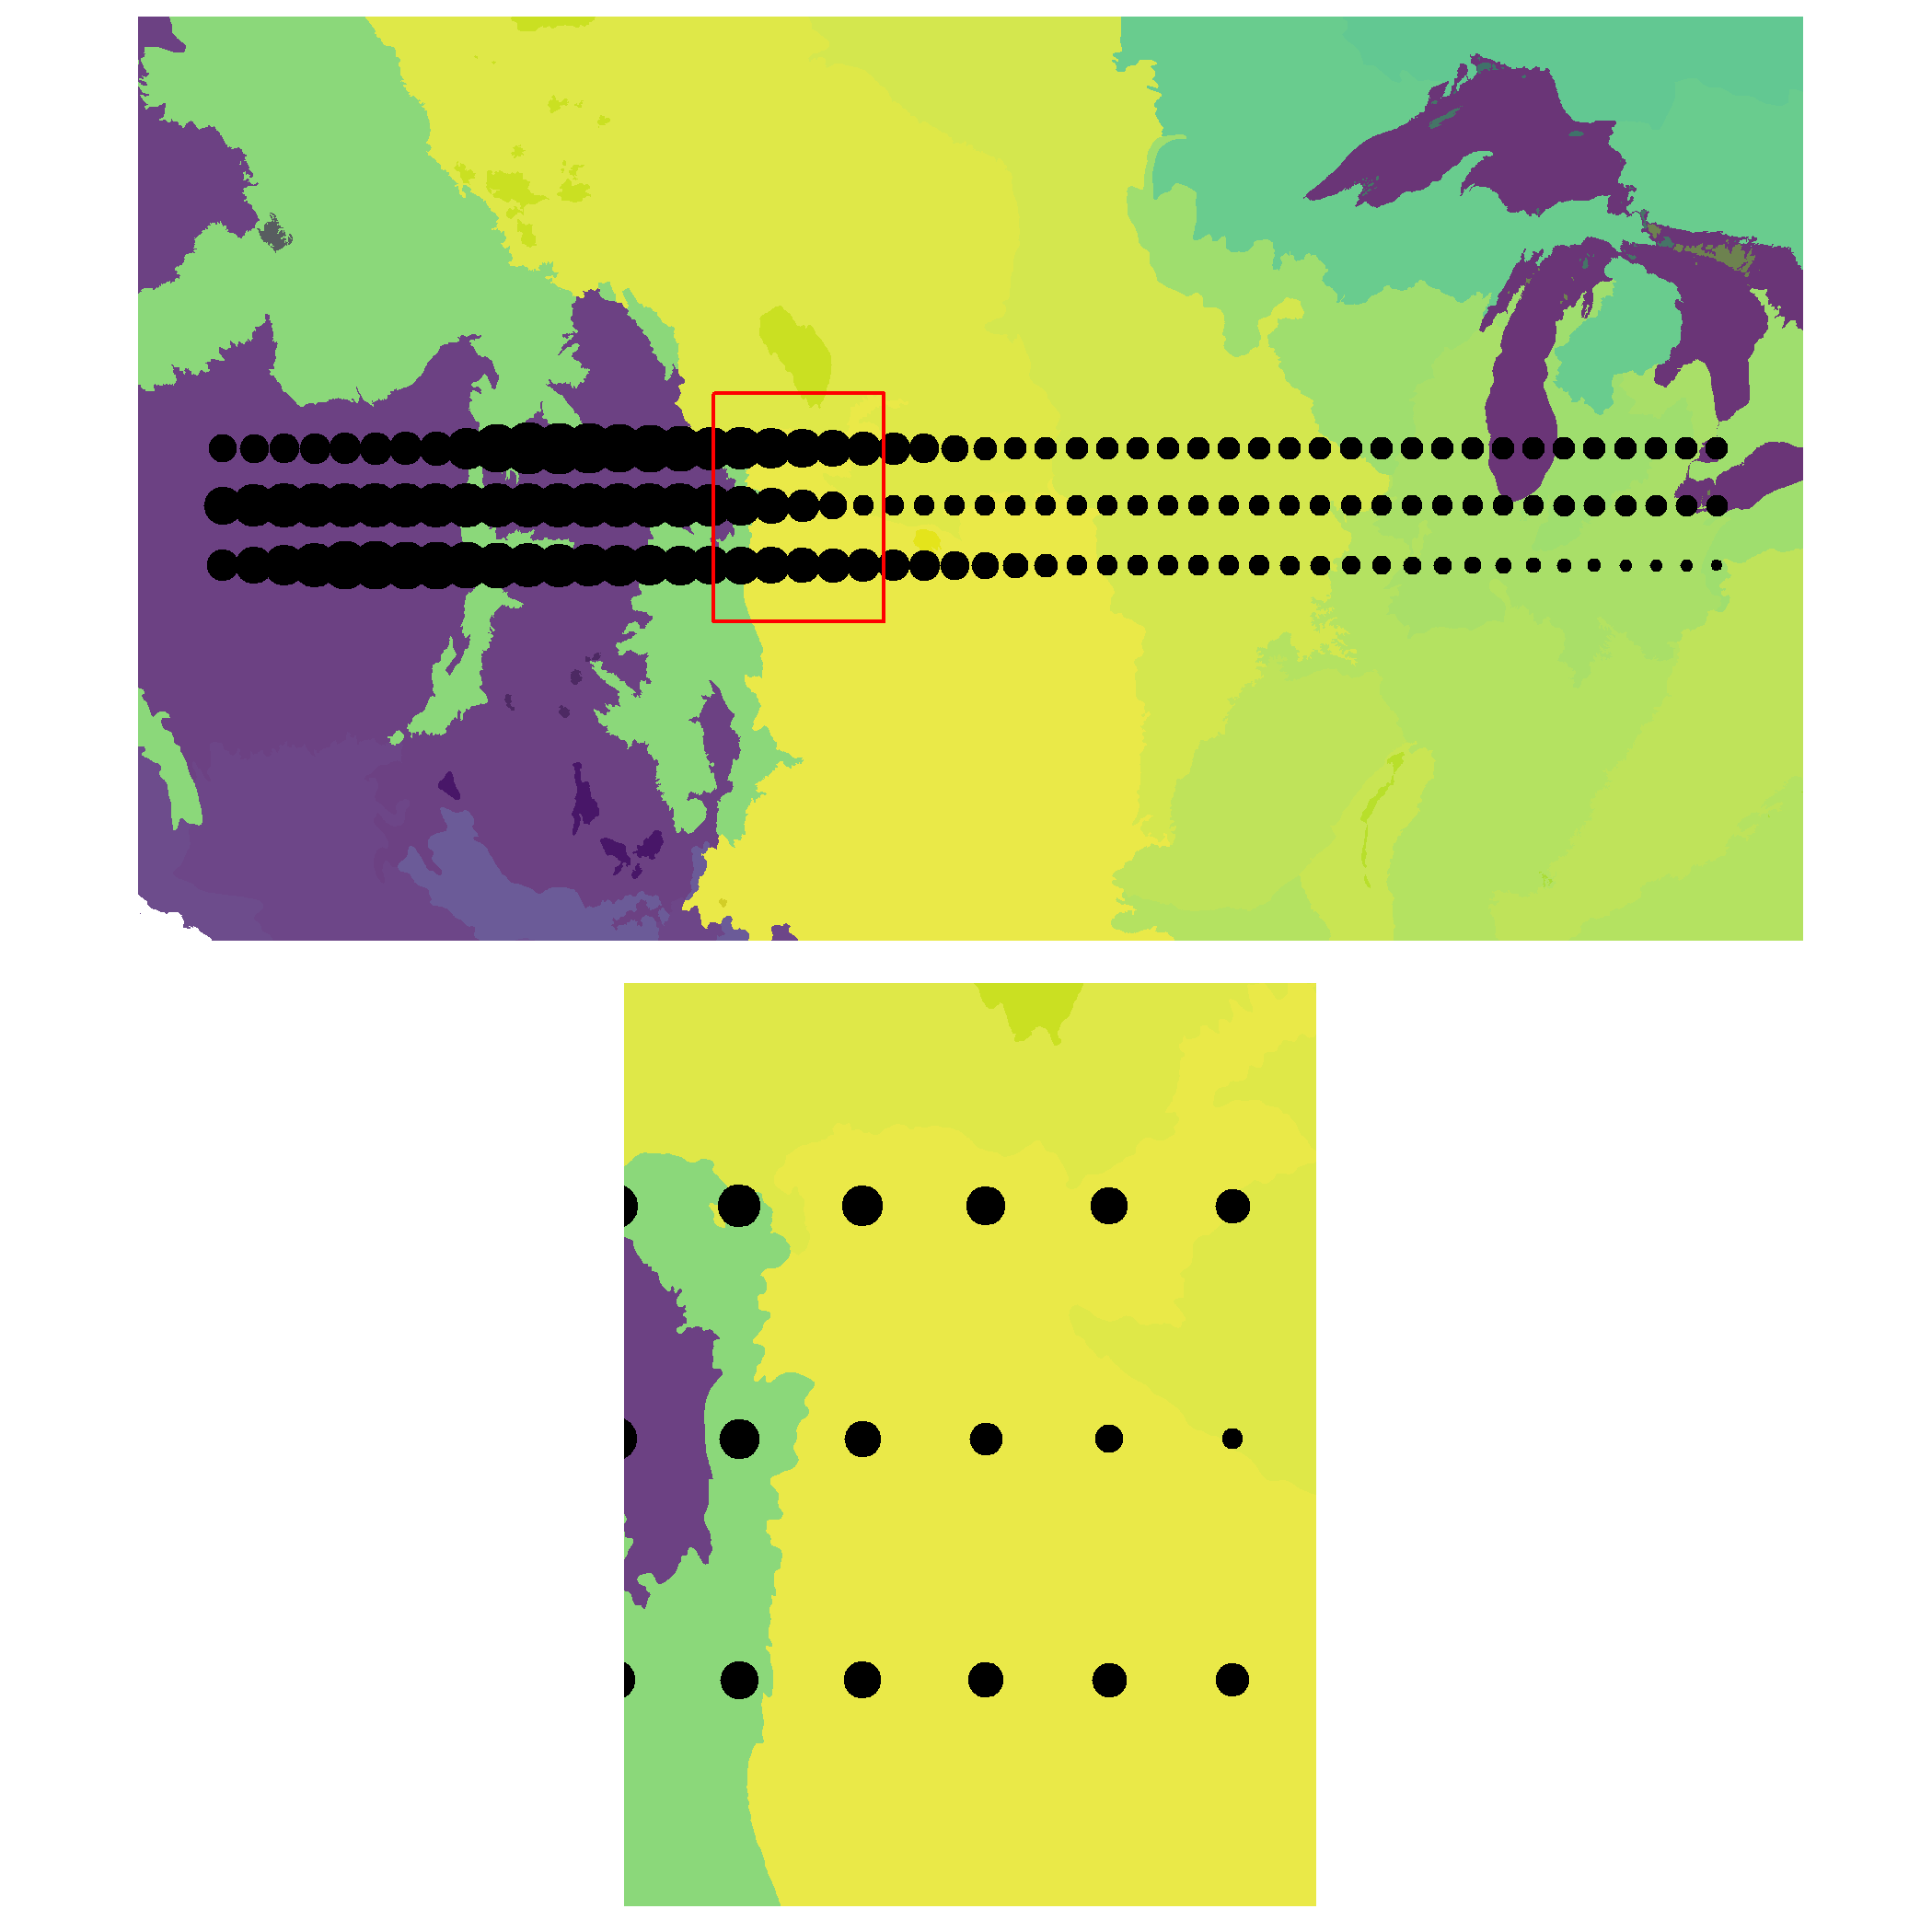
\includegraphics[width=0.85\linewidth]{./chapterFiles/fisherSpatial/figures/figsCalledInDiss/scaledFiInterpolated_year2010_zoom_East-West} 

}

\caption{No patterns of abrupt change detected in Fisher Information along three transects in year 2010}\label{fig:fiEcoregion}
\end{figure}
Upon initial investigation, there are no obvious signs of broad-scale patterns in FI across space (Fig. \ref{fig:fiEcoregion})\footnote{Size indicates value of Fisher Information (values are scaled and centered within transects). Red box (in top panel) indicates extent of bottom panel.}. If Fisher Information is an indicator of spatial regime boundaries, we should expect to see large changes in its value (in either direction) near the edges of functional spatial boundaries (e.g., at the boundaries of ecoregions). No clear regime changes appeared in areas where we might expect rapid changes (e.g., along the 105th meridian West, where a sharp change in altitude occurs).

Numerical investigation of the spatial correlation among adjacent transects also yielded no clear patterns. I did not identify any obvious correlation with changes in FI values and functional potential (using Omernick Ecoregion Level 2; see Fig. \ref{fig:fiEcoregion}). Rather than abrupt changes in Fisher Information I found graduaal changes (e.g., see results for years 2000 and 2010 in Figs. \ref{fig:fiEcoregion00},\ref{fig:fiEcoregion}).
\begin{figure}[h]

{\centering 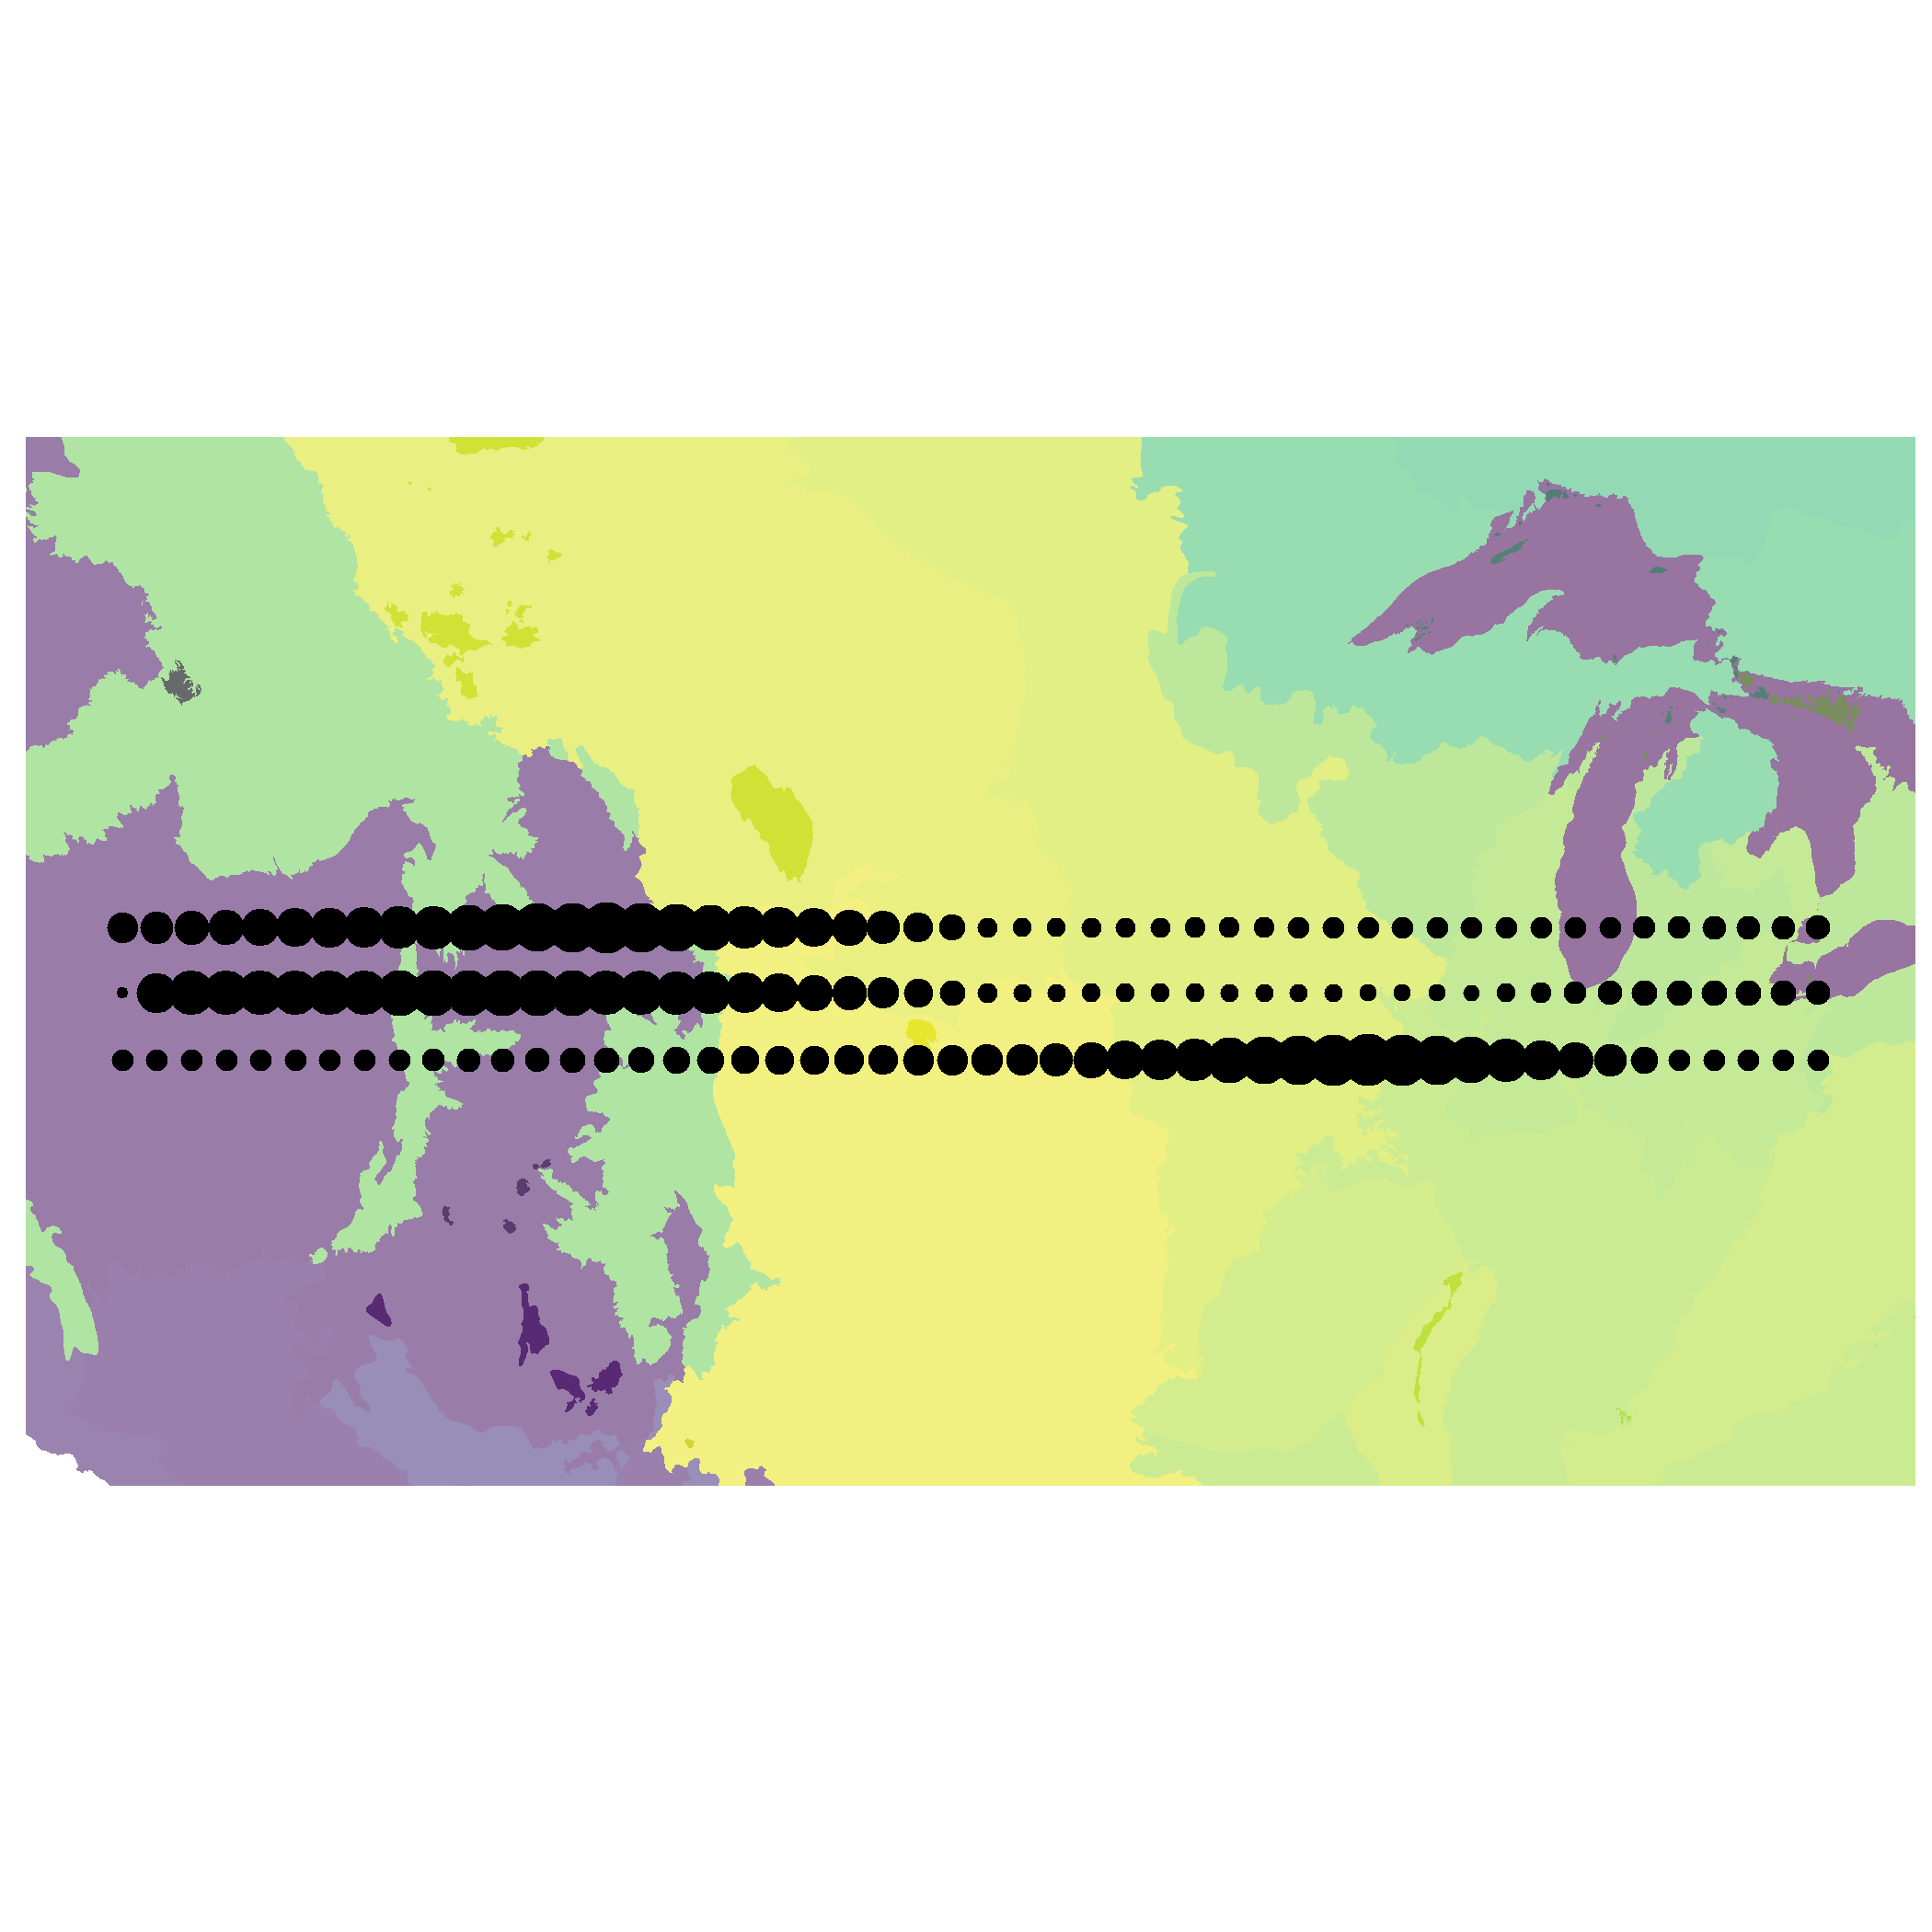
\includegraphics[width=0.85\linewidth]{./chapterFiles/fisherSpatial/figures/figsCalledInDiss/scaledFiInterpolated_year2000_East-West} 

}

\caption{Fisher Information (scaled and centered; point size positively correlated with value) against ecoregion boundaries (EPA Level 2).}\label{fig:fiEcoregion00}
\end{figure}
\hypertarget{discussion-1}{%
\section{Discussion}\label{discussion-1}}

The Fisher Information measure was introduced as a method to avoid some analytical issues related to complex and noisy ecological data (Karunanithi et al., 2008), and has also been suggested as an indicator of \emph{spatial} regimes (Sundstrom, Eason, Nelson, Angeler, Barichievy, Garmestani, Graham, et al., 2017a). I found no evidence suggesting Fisher Information {[}Eq. \eqref{eq:derivativesFI}{]} can identify `spatial regimes'. Further, the absence of autocorrelation among spatially adjacent transects suggests Fisher Information may not be a realiable indicator of changes in bird community structure.

Although the Fisher Information equation {[}Eq. \eqref{eq:derivativesFI}{]} used in this study is a relatively straightforward and fairly inexpensive computational calculation, extreme care should be taken when applying this index to ecological data. Fisher Information is capable of handling an infinite number of inputs (variables), and given sufficiently low window size paramters, can technically calculate an index value for only two observations. It is important that the user understands the assumptions of identifying 'regime shifts; using Fisher Information, since the efficacy of this method has not been yet subjected to rigorous tests (but see @ref(???ResamplingCHapter???)). There are three primary assumptions required when using Fisher Information to estimate relative orderliness within ecological data (Mayer et al., 2007):\\
1. the order or state(s) (\(s\)) of the system is observable,
1. any observable change in the information observed in the data represents reality and the variables used in the analyses will not produce false negatives, and
1. changes in \(I\) presumed to be regime shifts do not represent the peaks of cyclic (periodic) patterns.

The first assumption is one of philosophical debate and is thus not controllable. To attempt to control for false negatives, the user should take caution in her choice of input variables. In the the case of a high dimensional data, relativization and/or variable reduction measures may be useful (Rodionov 2005). However, Fisher Information does not convey information on how specific variables relate to the calculated index. Finally, we can take measures to account for cyclic behavior in the data by ensuring integration periods capture at one full cycle of the system and, given sufficently high number of observations, increasing the integration period may also alleviate some issues related to irreducible error (white noise).

The lack of patterns identified using Fisher Information may be influenced by one or more of the following: (1) the Breeding Bird Survey data collection scheme was designed to estimate and track \textbf{species} trends and not changes in entire communities; (2) these data consist of \textless{} 50 time points, and for some BBS routes much fewer. Ecological processes affecting large regions in this study area (e.g., the Central Great Plains) operate on larger time scales (i.e., \textgreater{}\textgreater{} 50 points). A mismatch among the ecologically relevant scales and the temporal resolution and extent of our data may influence the ability of this index to capture large-scale changes in whole bird communities.

Aside from the typical biases associated with the BBS data (e.g., species detection probability, observer bias), there are additional considerations to be made when using these data to identify `spatial regimes'. Breeding Bird Survey routes are spaced apart so as to reduce the probability of observing the same individuals, but birds which fly (especially in large flocks) overhead to foraging or roosting sites have a higher probability of being detected on multiple routes. We have, however, removed these species (waders, shorebirds, waterfowl, herons) from analysis. Regardless, this study assumes there is potential for each unique BBS route to represent its own state. If routes were closer together, it is more probable that the same type adn number of species would be identified on adjacent routes. Therefore, if this method does not detect slight changes in nearby routes which occupy the same `regime', then it follows that the method is sensitive to loss or inclusion of new species, which are spatially bounded by geological and vegetative characteristics. What new information does this give us about the system? Fisher Information reduces and removes the dimensionality of these middle-numbered systems, which omits critical information.

Effective regime detection measures should provide sufficient evidence of the drivers and/or pressures associated with the identified regime shifts (Mac Nally et al., 2014). The Fisher Information index collapses a wealth of data into a single metric, thereby foregoing the ability to relate state variables to the observed changes in Fisher Information, unlike other dimension reduction techniques. For example, loadings, or the relative influence of variables on the ordinated axes, can be derived from a Principal Components Analysis--this cannot be achieved using Fisher Information. If Fisher Information clearly suggested a spatial regime boundary or shift, a before-and-after post-hoc analysis of the regional community dynamics might confirm the regime shift occurrence.

\hypertarget{efficacy-of-fisher-information-as-a-spatial-rdm}{%
\subsection{Efficacy of Fisher Information as a spatial RDM}\label{efficacy-of-fisher-information-as-a-spatial-rdm}}

This study found no evidence suggesting Fisher Information accurately and consistently detects spatial boundaries of avian communities. Rapid changes in either direction of Fisher Information is suggested to indicate of a regime shift (Mayer, Pawlowski, \& Cabezas, 2006, @eason\_evaluating\_ 2012). Although this interpretation has been applied to multiple case studies of Fisher Information, there is yet a statistical indicator to objectively identify these abrupt changes. After calculating the Fisher Information for each spatial transect (Fig. \ref{fig:ewRoutesUsedHere}) during each sampling year, I used pairwise correlation to determine whether spatial autocorrelation existed among pairs of spatial transects. If some set of points are close in space and are \emph{not} separated by some physical or functional boundary (e.g., an ecotone, high altitude rock formations), then the Fisher Infomration calculate should exhibit a relatively high degree of spatial autocorrelation that is consistent over time. It follows that the correlation coefficient of spatially adjacent transects should be similar, diverging only as the distance beteween the transects differs and/or a functional or physical boundary separates them.

Several questions remain regarding the efficacy of Fisher Information as a regime detection measure in both spatial and temporal data. If signals of regime shifts do exist, it is clearly not possible to identify them using visual interpretation. I also did not find evidence to suggest spatial autocorrelation of the calculations. I suggest future studies of Fisher Infomration focuses on temporal, rather than spatial data. Potential areas of research and questions include:
1. Relationship of Fisher Information to likelihood ratio-based unsupervised change-point detection algorithms (e.g., ChangeFinder (Liu, Yamada, Collier, \& Sugiyama, 2013)).
1. Sensitivity of Fisher Information to data quality and quantity {[}this is explored in Chapter \ref{resampling}{]}.
1. What, if any, advantages does FI have over other density estimation techniques?\\
1. Does FI provide signals in addition to or different than geophysical and vegetative (e.g.~LIDAR) observations (data)?

\hypertarget{resampling}{%
\chapter{Data Quality Impacts on Regime Detection Measures}\label{resampling}}

\hypertarget{introduction-3}{%
\section{Introduction}\label{introduction-3}}

Ecological systems have many unpredictable and variably interacting components (Jørgensen et al.~2011). Methods for analyzing these complex systems, e.g.~Dynamic Bayesian Networks, network models, and food webs are designed to handle these complexities, yet require data- and knowledge-intensive models. Although ecological data collection and data management techniques are improving (La Sorte et al.~2018), the aforementioned approaches to modeling and understanding complex system are often infeasible in ecosystem research and management (Clements et al.~2015).

A growing concern with anthropogenic impacts on the environment has increased the demand for mathematical and statistical techniques that capture these dynamics. These often undesirable changes in the structure or functioning of ecological systems are often referred to as ``regime shifts'', ``regime changes'', ``state change'', ``abrupt change'', etc. (Andersen et al.~2009) . A yet-unattained goal of ecological research and management is to reach a point where these methods can predict impending regime shifts in real-time and with high confidence. Ideally, ecological regime shift detection methods (hereafter, RDMs) would require little knowledge of the intrinsic drivers of the system, and the users of the method would not be required to know if and where a regime shift occurred in the data.

Despite the suite of RDMs in the environmental and ecological research literatures, they are not used in ecological management. We can describe the current state of RDMs as being either system--specific (i.e., the method is not widely applicable or generalizable across systems) or not. Methods of the latter type are convenient in that they can be applied across various system and data types, but the results of these analyses require some degree of subjective interpretation (Clements and Ozgul 2018; c.f. Batt et al.~2013). Efforts to develop and/or improve RDMs that can handle these biases will aid the advance of RDMs research and application.

Current efforts to improve RDMs may be stunted by the lack of application beyond simple and/or theoretical (toy) systems data. Like most statistical and mathematical approaches, the evolution of many RDMs begins with application to theoretical data, followed by application to empirical data. Current applications of RDMs to empirical, ecological data are largely limited to data describing populations (e.g., Anderson and Piatt 1999, Alheit et al.~2005, deYoung et al.~2008), climatic, marine (e.g., Lipizer et al.~n.d., Nicholls 2011), and Paleolithic regime shifts (Spanbauer et al.~2014, Yang et al.~2017, Kong et al.~2017), with few applications terrestrial data (c.f. Bahlai et al.~2015, Sundstrom et al.~2017). Although testing the performance and inference boundaries of theoretical and simple systems is important, they are of little use to ecosystem managers if they are not proven to be easily and reliably applicable to their system. Additionally, RDMs should be capable of handling diverse and often noisy field data.

Ecological systems data is not only expensive and is difficult to capture, but is also notoriously imperfect---that is, process and observation error are common in these data. The resulting variability in data quality and quantity limits the numerical tools available for detecting ecological regime shifts (Thrush et al.~2009). Some methods, new and old, are proposed in the literature as RDMs which are capable of handling data limitation and quality issues inherent in ecological data and require few subjective decisions for choosing state variables and interpreting results. For example, variable reduction techniques, e.g.~principal components analysis (Rodionov 2005, Andersen et al.~2009, Reid et al.~2016) and clustering algorithms (Weijerman et al.~2005, Weissmann and Shnerb 2016), an index of variance (Brock and Carpenter 2006) and Fisher Information (Cabezas and Fath 2002, Fath and Cabezas 2004, Karunanithi et al.~2008) were introduced as methods which collapse the system into a single indicator of ecological regime shifts.

The transferability of RDMs to practitioners can only be facilitated by identifying intuitive metrics and testing the capacity of RDMs to handle high dimensional, empirical data. Here, we present a method for tracking the trajectory of an n-dimensional system using a single metric and its derivative. Here, I describe provide a description of this metric and apply it to empirical systems data. I then compare the results of this new metric to two other multivariate, model-free metrics: the Variance Index ({\textbf{???}}) and Fisher Information {[}({\textbf{???}}); \ref{fiGuide}{]}. Finally, we explore how decisions made during the data collection and data analysis phases impact these metrics.

\hypertarget{methods-1}{%
\section{Methods}\label{methods-1}}

\hypertarget{study-system-and-data}{%
\subsection{Study system and data}\label{study-system-and-data}}

I used paleodiatom time series from a freshwater system in North America which exhibited a rapid shift in community dynamics. These data were collected using a sediment coring method (see {\textbf{???}}). Community profiles at various depths within sediment cores are analyzed to obtain relative abundances. Relative abundances at various depths within the sediment core are then related to time (years before present) using carbon dating techniques. These data can be obtained from the publisher's website.

In Chapter \ref{velocity}, I described a `new' method, \textbf{system velocity}, as a potential dimension reduction and regime detection method. Although this is the first instance of this calculation to, alone, be suggested as a regime detection metric, it has been used as part of a larger series of calculations of the Fisher Information metric (see also \ref{fiGuide}). First introduced in by Fath et al. (2003) as one of multiple steps in calculating their variant of Fisher Information, system velocoty represents the cumulative sum of the squared change in all state variables over a period of time. Steps for calculating this metric are described below.

\hypertarget{results-2}{%
\section{Results}\label{results-2}}

SEE IIASA REPORT

\hypertarget{discussion-2}{%
\section{Discussion}\label{discussion-2}}

\hypertarget{ackowledgements}{%
\section{Ackowledgements}\label{ackowledgements}}

This study was conceptualized at the International Institute for Applied Systems Analysis (IIASA) as part of the Young Scholars Summer Program in 2018. I thank my IIASA program supervisors, Drs. Brian Fath and Elena Rovenskaya, for advisement during this period and for comments on an earlier version of this chapter.

\hypertarget{velocity}{%
\chapter{\texorpdfstring{Velocity (\emph{v}): rate-of-change of system trajectory as a potential indicator of abrupt change}{Velocity (v): rate-of-change of system trajectory as a potential indicator of abrupt change}}\label{velocity}}

\hypertarget{introduction-4}{%
\section{Introduction}\label{introduction-4}}

Dimension reduction techniques and RDms blablbah
In this Chapter I describe the steps for calculating a `new' metric, \textbf{system velocity}, for reducing the dimensionality and identifying abrupt shifts in high dimensional data. Although this is the first instance of this calculation to, alone, be suggested as a regime detection metric, it has been used as part of a larger series of calculations of the Fisher Information metric {[}see \ref{fiGuide}{]}, first introduced in Fath et al. (2003). Below, I describe the steps for calculating system velocity, simply defined as the cumulative sum of the squared change in all state variables over a period of time.

\hypertarget{about-the-toy-system}{%
\section{About the toy system}\label{about-the-toy-system}}

Consider a system (Fig. \ref{fig:sysEx}) with \(N\) state variables (\(x_i\)), with observations taken at time points, \(t\). System velocity is calculated as the cumulative sum over time period \(t_0\) to \(t_j\), as the total change in all state variables, \{\(x_1 ...x_N\)\}, between two adjacent time points, e.g., \(t_j\) and \(t_{j+1}\), denoted \(t_{j,j+1}\). I use a simple, two-variable system to demonstrate the calculation of each step below. The system comprises variables \(x_1\) and \(x_2\), with observations occurring at each time point \(t = {1,2,3,...100}\).
\begin{figure}[h]

{\centering 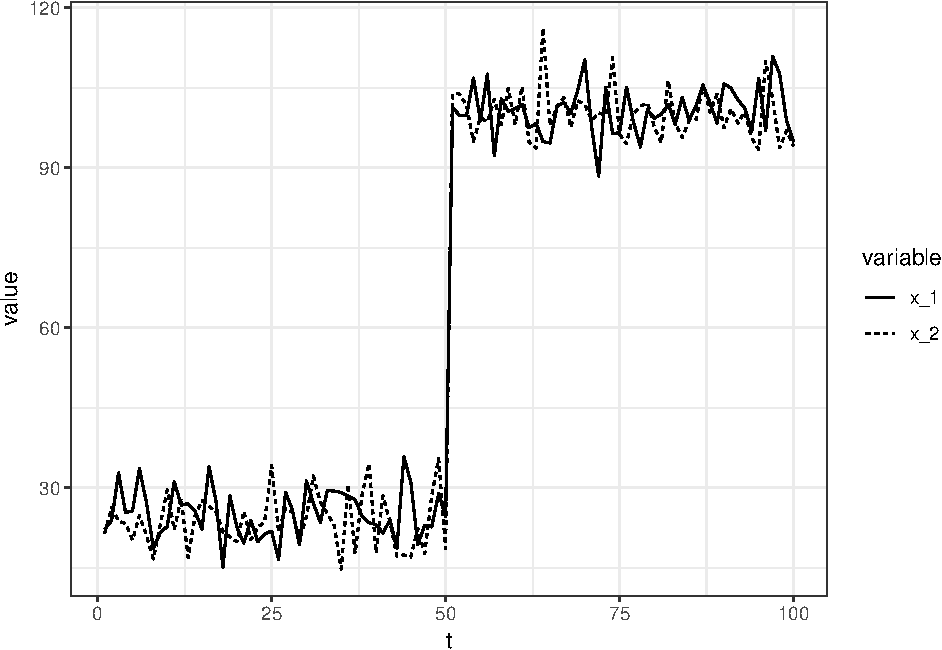
\includegraphics[width=0.95\linewidth]{_myDissertation_files/figure-latex/sysEx-1} 

}

\caption{The 2-variable toy system used to demonstrate steps for calculating system velocity. Each variable, $x$, is drawn from a normal distribution with means that change at $t = 50$. State variables have constant variance $\sigma = 5$. }\label{fig:sysEx}
\end{figure}
\hypertarget{steps-for-calculating-system-velocity-v}{%
\section{\texorpdfstring{Steps for calculating system velocity, \emph{v}}{Steps for calculating system velocity, v}}\label{steps-for-calculating-system-velocity-v}}

First, we calculate the change in each state variable, \(x_i\), between two adjacent points in time, \(t_j\) and \(t_{j+1}\), such that the difference, \(x_{t_{j+1}} - x_{t_j}\) is assigned to the latter time point, \(t_{j+1}\). For example, in our toy data, we use observations at time points \(t = 1\) \& \(t=2\) (Fig. \ref{fig:sysEx2}). For all examples in this chapter, the state variables \(x_1\) and \(x_2\) were drawn from a normal distribution (using function \emph{rnorm}), with parameters \(\bar{x}_i\) (mean) and \(\sigma_i\) (sd) for 100 time steps, \(t\). The regime shift occurs at \(t=50\), where a shift in either or both \(\bar{x}_i\) or \(\sigma_i\).

\hypertarget{step-1-delta-x_i}{%
\subsubsection{\texorpdfstring{Step 1: \(\Delta x_i\)}{Step 1: \textbackslash{}Delta x\_i}}\label{step-1-delta-x_i}}

The first step in calculating \(v\) is to obtain the change in values for each state variables, \(x_1\) and \(x_2\) between two consecutive time points (e.g., from \(t=1\) to \(t=2\):
\begin{equation}
\begin{array}{rcr}
\Delta x_1 = x_{1_{t=2}} - x_{1_{t=1}} \\
\Delta x_2 = x_{2_{t=2}} - x_{1_{t=1}}
  \end{array}
\label{eq:diffX}
\end{equation}
\begin{figure}[h]

{\centering 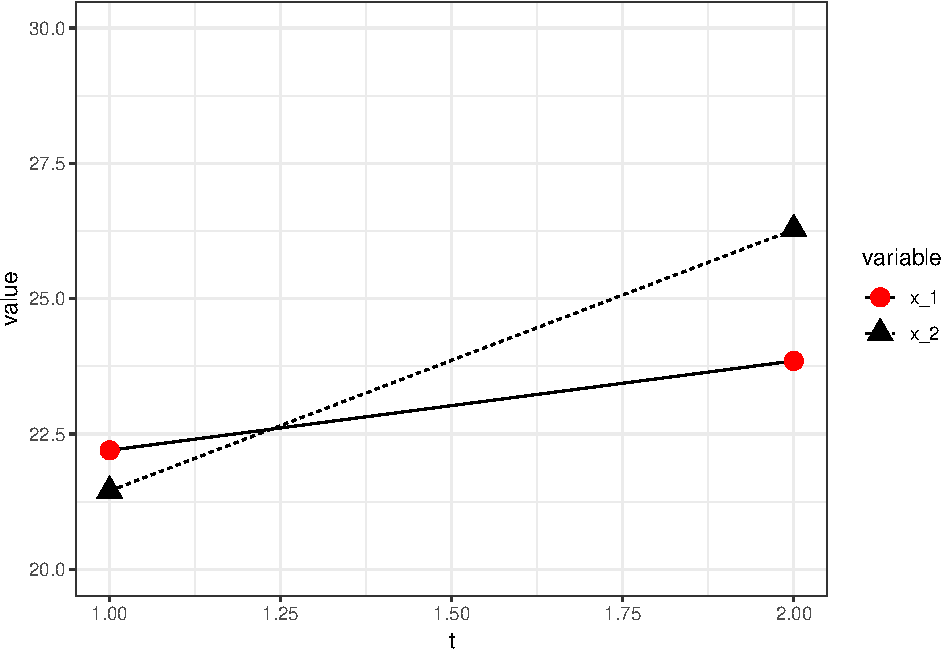
\includegraphics[width=0.95\linewidth]{_myDissertation_files/figure-latex/sysEx2-1} 

}

\caption{Data used to calculate velocity at the first two time points, $t_1$ and $t_2$.}\label{fig:sysEx2}
\end{figure}
\hypertarget{step-2-sqrtsum_indelta-x_12}{%
\subsubsection{\texorpdfstring{Step 2: \(\sqrt(\sum_i^N\Delta x_1^2)\)}{Step 2: \textbackslash{}sqrt(\textbackslash{}sum\_i\^{}N\textbackslash{}Delta x\_1\^{}2)}}\label{step-2-sqrtsum_indelta-x_12}}

After calculating the differences for each state variable, we will next calculate the total change in the system over the time elapsed, following Pythagora's theorem,
\begin{equation}
 X_1^2 + X_2^2 = s^2 
  \label{eq:pythagorean}
\end{equation}
where \(s\) represents the total change in the system, and \(X_1\) and \(X_2\) represent the changes in all state variables (\(x_{i_{t=2}} - x_{i_{t=1}}\)). We achieve this by first squaring the differences obtained in Eq. \eqref{eq:diffX}:
\begin{equation}
\begin{array}{rcr}
(x_{1_{t=2}} - x_{1_{t=1}})^2  \\
(x_{2_{t=2}} - x_{2_{t=1}})^2 
\end{array}
  \label{eq:diffXsq}
\end{equation}
\hypertarget{step-3-use-pythagorean-theorem-to-isolate-s}{%
\subsubsection{\texorpdfstring{Step 3: Use Pythagorean theorem to isolate \(s\)}{Step 3: Use Pythagorean theorem to isolate s}}\label{step-3-use-pythagorean-theorem-to-isolate-s}}

Next, we isolate \(s\) in Eq. \eqref{eq:pythagorean}, capturing the total change in all state variables into a single measure by taking the 2nd root of the squared sums of all \(x\):
\begin{equation}
\begin{array}{rcr}
\sum_{i=1}^{N} \Delta {x_i} = \sum_{i=1}^{N}(x_{t_{i+1}} - x_{t_i})^2 \\ 
\ = \Delta s \\ 
\ = \sqrt([x_{1_{t=2}} - x_{1_{t=1}}]^2 + [x_{2_{t=2}} - x_{2_{t=1}}]^2)
\end{array}
\label{eq:diffXsq2}
\end{equation}
We now have a single measure, \(\Delta s\) (Eq. \eqref{eq:diffXsq2}), for each pair of time points in our \(N\)-dimensional system. It is obvious that \(\Delta s\) will always be a positive value, since we took the 2nd root of a squared value. Although discussed in a later section, it is important to note that this value is not unitless--that is, our example system takes on the units of our state variables, \(x_1\) and \(x_2\). Because we are interested in identifying abrupt changes in the entire system, we calculate the cumulative sum of \(\Delta s\) at every time point, such that:
\begin{equation}
s = \sum_{t=1}^T \Delta s
\label{eq:s}
\end{equation}
\#\#\#\# Step 4: Calculate velocity, \(v\) (or \(\frac {\Delta s}{\Delta t}\))
Finally, we calculate the \textbf{system velocity}, \(v\) (or \(\frac{\Delta s}{\Delta t}\)), by first calculating the change in \(s\) (Eq. \eqref{eq:s}), and then divide by the total time elapsed between consecutive sampling points:
\begin{equation}
 v = \frac {s_{t+1}-s_{t}}{\Delta t} 
\label{eq:velocity}
\end{equation}
\begin{figure}[h]

{\centering 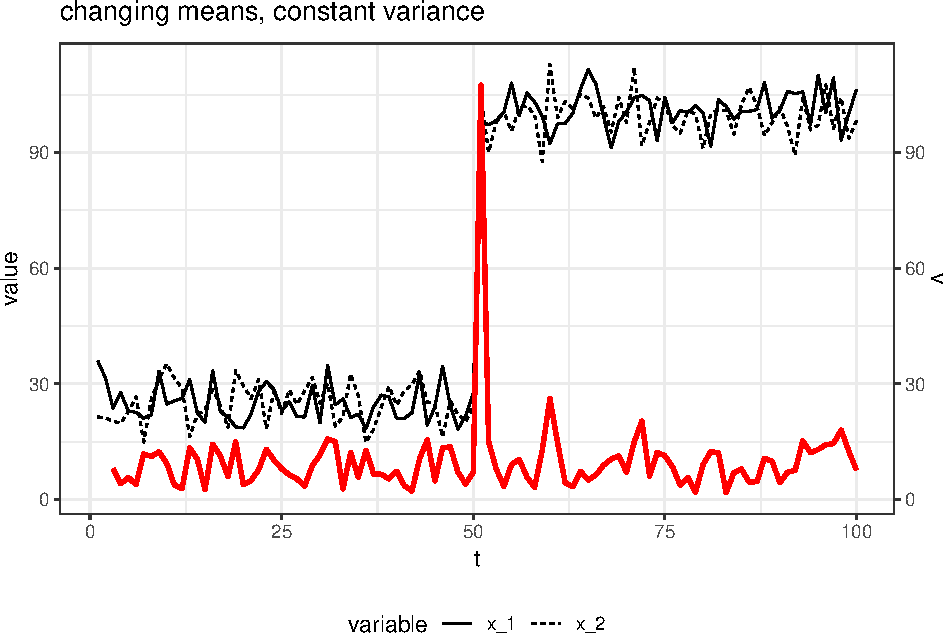
\includegraphics[width=0.95\linewidth]{_myDissertation_files/figure-latex/velocSysEx1-1} 

}

\caption{System change ($s$) and velocity ($v$) of the model system over the time period. Constant means ($\bar{x}_{pre}=25$, $\bar{x}_{post}=10$) and sharp change in variance for both state variables, $\sigma =5$.}\label{fig:velocSysEx1}
\end{figure}
The steps for calculating velocity {[}Eq. \eqref{eq:velocity}{]} are demonstrated using the first five time points of our toy system (Fig. \ref{fig:sysEx}) in Table \ref{tab:distTab}.

\hypertarget{velocity-v-performance-under-varying-mean-and-variance-in-the-toy-system}{%
\section{\texorpdfstring{Velocity \emph{v} performance under varying mean and variance in the toy system}{Velocity v performance under varying mean and variance in the toy system}}\label{velocity-v-performance-under-varying-mean-and-variance-in-the-toy-system}}

I simulated 10,000 random draws of the toy system, which experiences a rapid shift at \(t = 50\), while varying two each of the following system paramters at the regime shift:
\(\bar{x}_1\), increased the mean value of \(x_1\)
\(\sigma_1\), change in variance of \(x_1\)
Simulations consisted of 10,000 random samples drawn from the normal distribution for each paramter, I randomly drew the toy system samples 10,000 times under increasing values of \(\bar{x}_1\) and \(\sigma_1\). To identify patterns in the influence of paramter values on velocity, I present the mean values of \(v\) across all simulations, with confidence intervals of \(\pm 2\) standard deviations. As mentione above, the state variables \(x_1\) and \(x_2\) were drawn from a normal distribution (using function \emph{rnorm}), with parameters \(\bar{x}_i\) (mean) and \(\sigma_i\) (sd) for 50 time steps, \(t\).

\hypertarget{varying-post-shift-mean}{%
\subsubsection{Varying post-shift mean}\label{varying-post-shift-mean}}

I examined the influence of the magnitude of change in \(x_1\) in the period before (pre; \(t <50\)) and after (post; \(t \geq 50\)) by varying the mean parameter, \(\bar{x}_1\) in the set \(W=\{25,30,35,...100 \}\) (Figs. \ref{fig:simVplot1},\ref{simVplot2}). As expected, the magnitude of \(v\) increased linearly as the total difference between \(\bar{x}_{1_{pre}}\) and \(\bar{x}_{1_{post}}\) increased (\ref{fig:simVplot2}). This is not surprising, as \(s\) increases as the total change in abundance across the entire sytem increases (Eq. \eqref{eq:s}), therefore, the potential maximum of \(v\) also increases. This may indicate that \(v\), while capable of identifying large shifts in data structure, may not pick up subtle changes (i.e.~lower effect sizes).
\begin{figure}[h]

{\centering 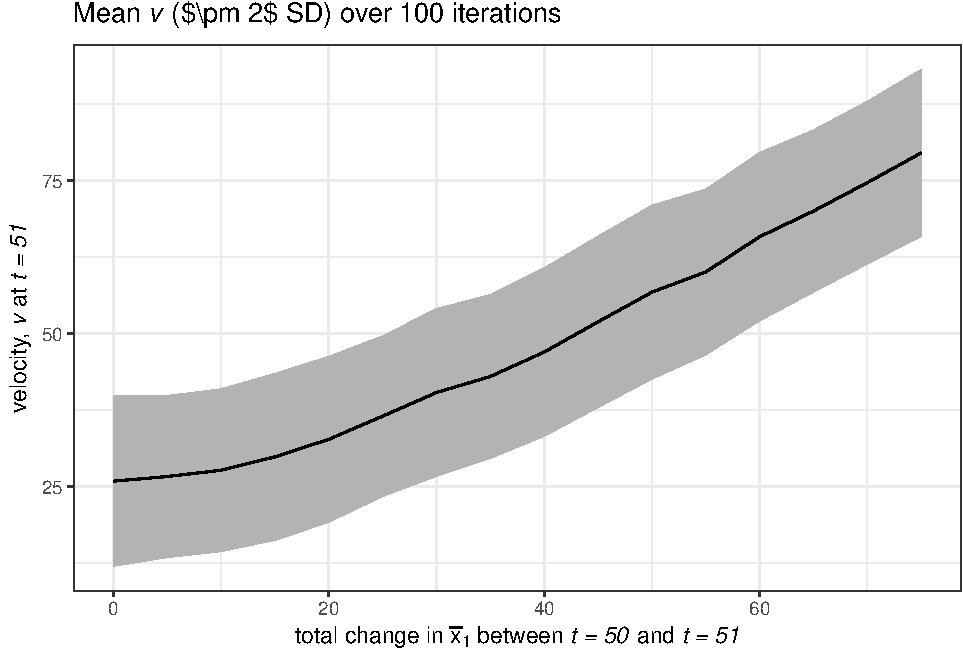
\includegraphics[width=0.95\linewidth]{_myDissertation_files/figure-latex/simVplot2-1} 

}

\caption{Change in velocity ($v$) as the total change in the mean value of $\bar{x}_{2_{t=50}}$ over 10,000 simulations. A regime shift was induced at $t=50$ with constant varoance $\sigma = 5$, $\bar{x}_2 = 25$ when $t<50$,  and changes in variable mean values, $\bar{x}_2 = 50$ when $t \geq 50$, $\bar{x}_1 = 25$ when $t<50$.}\label{fig:simVplot2}
\end{figure}
\hypertarget{varying-post-shift-variance}{%
\subsubsection{Varying post-shift variance}\label{varying-post-shift-variance}}

In the previous example, variance was constant before and after the shift at \(t=50\). To determine whether the signal emitted by \(v\) at the regime shift is lost with increasing variance, I varied the variance parameter, \(\sigma_1\) in the set \(W = \{1,2,3,...25 \}\). The variance for both state variables prior to the regime shift, \(\sigma_1\) and \(\sigma_2\), was 5, with the change occurring in \(\sigma_1{_{post}}\). Sytem velocity \(v\) appears senstive to increases in the variance at the point of the regime shift (Figs. \ref{fig:simVarplot}, \ref{fig:simVarplot2}). This extreme sensitivity of \(v\) to \(\sigma{_{post}}\) (Fig. \ref{fig:simVarplot2}) is unsurprising, given the fact that, without smoothing the derivatives, the tangential speed of a `noisy' variable will always be noisy itself (see Figs. \ref{velocitySysEx1}, \ref{velocitySysEx2}, \ref{velocitySysEx3}, \ref{velocitySysEx4}).
\begin{figure}[h]

{\centering 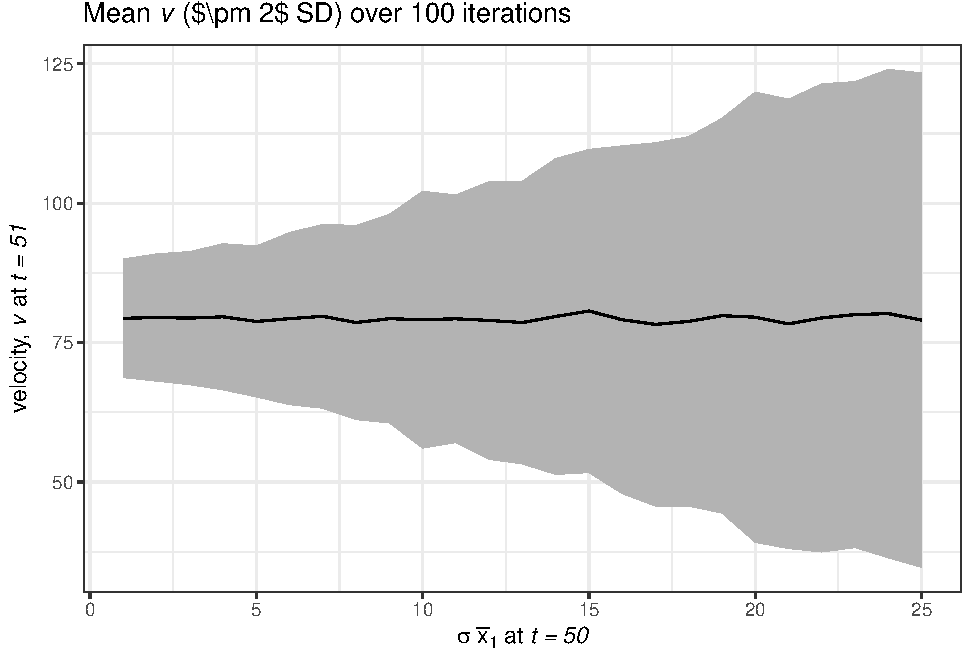
\includegraphics[width=0.95\linewidth]{_myDissertation_files/figure-latex/simVarPlot2-1} 

}

\caption{Average ($\pm 2$ SD) velocity ($v$) woresens as the variance of $\bar{x}_{2_{t=50 (post)}}$ (post shift) increases. $\bar{x}_{1_{pre}} = 25$, $\bar{x}_{1_{post}} = 100$, $\bar{x}_{2_{pre}} = 25$, $\bar{x}_{2_{post}} = 50$, $\sigma_{1_{pre}} = 5$, $\sigma_{2_{pre,post}} = 5$}\label{fig:simVarPlot2}
\end{figure}
\hypertarget{smoothing-the-data-prior-to-calculating-v}{%
\subsubsection{\texorpdfstring{Smoothing the data prior to calculating \emph{v}}{Smoothing the data prior to calculating v}}\label{smoothing-the-data-prior-to-calculating-v}}

To ameliorate the influence of noise (e.g.~Fig. \ref{simVarPlot}) on the regime shift signal in \(v\), I used linear approximation techniques in attempt to smooth the velocity (derivatives). I used the function \emph{stats::approx} to interpolate values of \(x_1\) and \(x_2\) to regularly-spaced time points in the set \(t=\{1:100\}\), and then calculated \(v\) as described in the steps above (Eqs. \eqref{eq:diffX}:\eqref{eq:velocity}). Increasing the number of points (\(t\)) at which the original state variables were smoothed did not influence the amount of noise surrounding the signal of the regime shift (at \(t=50\)) in system velocity, \(v\) (Fig. \ref{fig:smoothV}).

\hypertarget{discussion-3}{%
\section{Discussion}\label{discussion-3}}

In this chapter, I described the steps for calculating a novel regime detection metric, system velocity (\(v\)). First described in Fath et al. (2003), \(v\) is used as a single step for caclulating a more complicated regime detection metric, Fisher Information (see also Chapter \ref{fiGuide}). System velocity is arguably simple to calculate, as shown in this chapter, captures the total change in system variables under a variety of mean and variance conditions. The metric does not, however, perform well as variance increases (Fig. \ref{simVarPlot2}), and smooothing the original data does not reduce the noise surrounding this metric when variance is moderate (Fig. \ref{smoothV}).

Variance is a commonly-used indicator of ecological regime shifts (Brock \& Carpenter (2006)), however, fails to perform when the number of variables is \textgreater{}\textgreater{} a few. System velocity, \(v\), may be useful in situations where the number of state variables is much greater than a few, and appears especially useful when the magnitude of change in one or more state variables is high (Fig. \ref{fig:simVplot2}). For example, this method will likely identify signals of regime shifts where the shift is defined as high species turnover within a community.

I tested the efficacy of this metric as an indicator of abrupt change in a two-variable system. Although a useful first step, this metric should be considered in a multi-species context, and particularly in community-level empirical data which is difficult to simulate. I demonstrate a compelling case study in materials associated with my R Package, \textbf{regimeDetectionMeasures}, and in Appendix \ref{appPaleo} in which multiple species turnover events are apparent in a paleodiatom community time series. In this case study, the `distance travelled', \(s\) (Eq. \eqref{eq:diffXsq2}), clearly exhibits shifts at points where expert opinion and species turnover (in species dominance) agree that a large change occurred. Further, velocity, \(v\) (see \emph{dsdt} in the package materials) indicates a large shift at only the most predonimnant shift in the time series, perhaps due to the metric's sensitivity to variance (Fig. \ref{fig:simVplot2}.

Further work is required to determine the utility of system velocity as a regime detection metric, however, this chapter demonstrates that the metric may indicate clear shifts in variable means. For multispecies data you will typically need to reduce dimensionality before you can proceed with analyses, for example using some sort of ordination. In addition to examining high-dimensional and noisy data, a study of the performance of \(v\) under conditions where few variables exhibit large changes while many variables are relatively constant may also prove useful. Additionally, this metric may be a useful tool for reducing the dimensionality of high dimensional data. Although the metric loses much information, as opposed to some dimension reduction techniques, e.g.~Principal Components Analysis PCA, the metric is simple to calculate (even by hand), is computationally inexpensive, and is intuitive, unlike many clustering algorithms (e.g., Non-metric Multidimensional Scaling NMDS). Like system velocity, methods of the latter variety (e.g.~NMDS) require post-hoc statistical analyses to confirm the location of clusters (or abrupt change, regime shifts), while methods of the former variety (e.g.~PCA) retain loadings but do not necessarily identify the locations of abrupt shifts.

\hypertarget{supplementary-materials}{%
\section{Supplementary Materials}\label{supplementary-materials}}
\begin{figure}[h]

{\centering 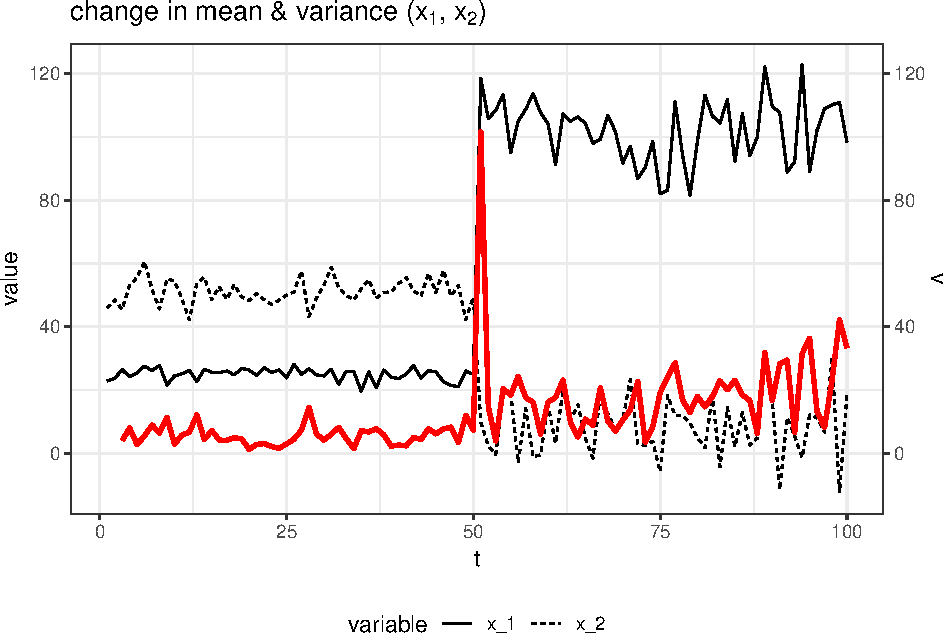
\includegraphics[width=0.95\linewidth]{_myDissertation_files/figure-latex/velocSysEx2-1} 

}

\caption{System change ($s$) and velocity ($v$) of the model system over the time period. Change in means ($\bar{x}_{1_{pre}}=25$, $\bar{x}_{1_{post}}=100$, $\bar{x}_{2_{pre}}=50$, $\bar{x}_{2_{post}}=10$) and an increase in variance ($\sigma_{1_{pre}}=2$, $\sigma_{1_{post}}=10$, $\sigma_{2_{pre}}=5$,  $\sigma_{2_{post}}=10$).}\label{fig:velocSysEx2}
\end{figure}
\begin{figure}[h]

{\centering 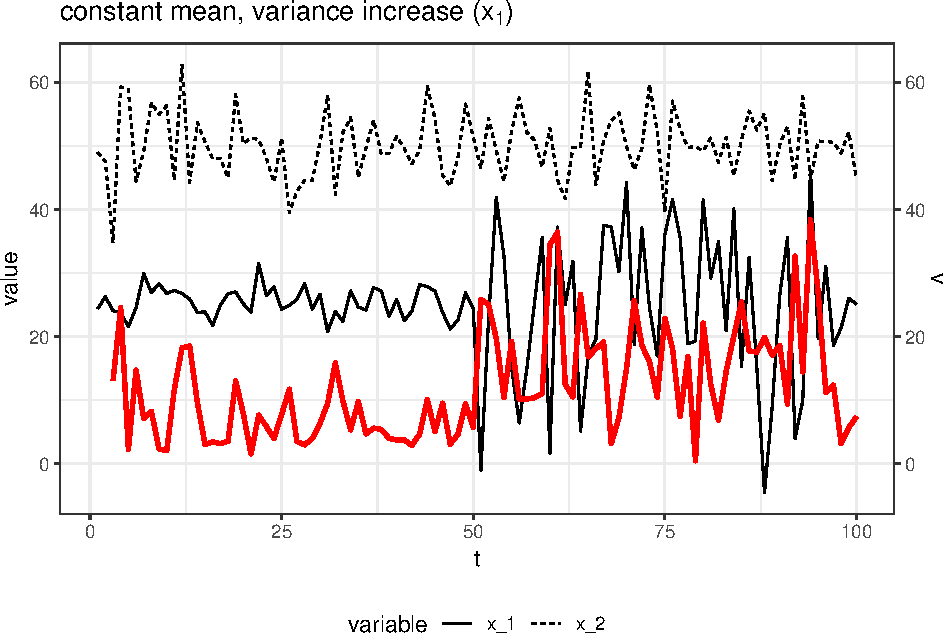
\includegraphics[width=0.95\linewidth]{_myDissertation_files/figure-latex/velocSysEx3-1} 

}

\caption{System change ($s$) and velocity ($v$) of the model system over the time period. Constant means ($\bar{x}_1=25$, $\bar{x}_2=50$) and sharp change in variance for one state variable $\sigma_{1_{pre}} = 2$, $\sigma_{1_{post}} = 12$, $\sigma_{2_{pre,post}} = 5$}\label{fig:velocSysEx3}
\end{figure}
\begin{figure}[h]

{\centering 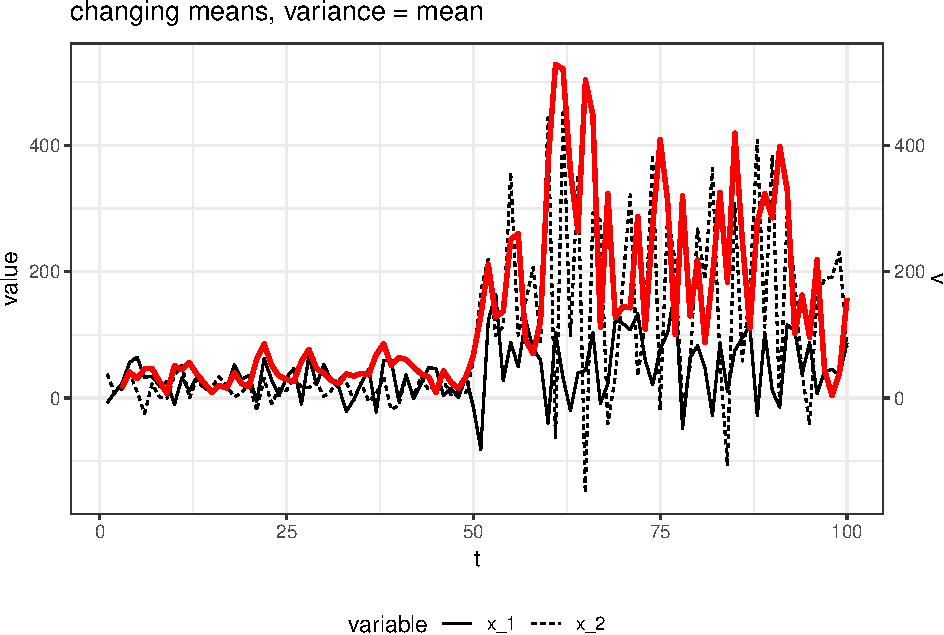
\includegraphics[width=0.95\linewidth]{_myDissertation_files/figure-latex/velocSysEx4-1} 

}

\caption{System change ($s$) and velocity ($v$) of the model system over the time period. Variance equal to mean ($\bar{x_i}=\sigma_i$), where means ($\bar{x}_{1_{pre}}=25$, $\bar{x}_{1_{post}}=50$, $\bar{x}_{2_{pre}}=15$, $\bar{x}_{2_{post}}=150$).}\label{fig:velocSysEx4}
\end{figure}
\appendix

\hypertarget{appPaleo}{%
\chapter*{Appendix: Distance travelled and velocity using a paleodiatom case study}\label{appPaleo}}
\addcontentsline{toc}{chapter}{Appendix: Distance travelled and velocity using a paleodiatom case study}

This appendix provides documentation and R code association with the paleodiatom community example.

\hypertarget{setup}{%
\section{Setup}\label{setup}}

\hypertarget{load-required-packages}{%
\subsection{Load required packages}\label{load-required-packages}}

You will need to install the following packages if they are not already.

\hypertarget{load-the-data}{%
\subsection{Load the data}\label{load-the-data}}

Pull in the data from the supplementary materials for Spanbauer \emph{et al.} (2014) (Spanbauer et al., 2014). This data contains the percent abundances of diatom species from Foy Lake. Spanbauer \emph{et al.} (2014) calculated the number of relative diatom valves in each sample. They removed time steps with no diatom data, claiming poor preservation rather than zero abundance. The authors also averages time steps 301 - 312.
\begin{Shaded}
\begin{Highlighting}[]
\NormalTok{data <-}\StringTok{ }\KeywordTok{read_csv}\NormalTok{(}\StringTok{"https://doi.org/10.1371/journal.pone.0108936.s001"}\NormalTok{)}
\end{Highlighting}
\end{Shaded}
\hypertarget{calculate-the-distance-metric}{%
\section{Calculate the distance metric}\label{calculate-the-distance-metric}}

\hypertarget{calculate-the-distance}{%
\subsection{Calculate the distance}\label{calculate-the-distance}}

Calculate the difference, \(\Delta x\), in each species' relative abundance from time \emph{n} to time \emph{n + 1}. Calculate the change in distance, \(\Delta s\), as the sum of the squares of the change in each species. Calculate the distance as the cummulative sums of the change in distance.

Load the numerical differentiation results data. These finite differences were approximated in MatLab, using code that implements the methods found in Chartrand, R. Numerical differentiation of noisy, nonsmooth data. (2011) ISRN Applied Mathematics, Vol. 2011. Article ID 164564 (Chartrand, 2011).

\hypertarget{dataframe-processing}{%
\subsection{Dataframe processing}\label{dataframe-processing}}

Create a dataset in `long' form for future plotting

\hypertarget{visualize-data-and-results}{%
\section{Visualize data and results}\label{visualize-data-and-results}}

\hypertarget{plot-the-relative-abundance-data-over-time}{%
\subsection{Plot the relative abundance data over time}\label{plot-the-relative-abundance-data-over-time}}
\begin{center}\includegraphics[width=0.95\linewidth]{_myDissertation_files/figure-latex/unnamed-chunk-12-1} \end{center}

\hypertarget{plot-the-distance-travelled}{%
\subsection{Plot the distance travelled}\label{plot-the-distance-travelled}}
\begin{center}\includegraphics[width=0.95\linewidth]{_myDissertation_files/figure-latex/unnamed-chunk-13-1} \end{center}

\hypertarget{plot-the-velocity}{%
\subsection{Plot the velocity}\label{plot-the-velocity}}
\begin{center}\includegraphics[width=0.95\linewidth]{_myDissertation_files/figure-latex/unnamed-chunk-14-1} \end{center}

\hypertarget{plot-the-acceleration}{%
\subsection{Plot the acceleration}\label{plot-the-acceleration}}
\begin{center}\includegraphics[width=0.95\linewidth]{_myDissertation_files/figure-latex/unnamed-chunk-15-1} \end{center}

\hypertarget{plot-a-histogram-of-distance-traveled}{%
\subsection{Plot a histogram of distance traveled}\label{plot-a-histogram-of-distance-traveled}}

Compare histogram of distance travelled to pdf calculated from velocity.
\begin{center}\includegraphics[width=0.95\linewidth]{_myDissertation_files/figure-latex/unnamed-chunk-16-1} \end{center}

\hypertarget{moving-window-analysis}{%
\section{Moving window analysis}\label{moving-window-analysis}}

\hypertarget{specifcy-parameters-for-the-moving-window}{%
\subsection{Specifcy parameters for the moving window}\label{specifcy-parameters-for-the-moving-window}}

Distance over which to move the window (in units time)
\begin{Shaded}
\begin{Highlighting}[]
\CommentTok{# Distance over which to move the window (in units time)}
\NormalTok{winspace <-}\StringTok{ }\DecValTok{50}

\CommentTok{# Size of the window (in units time)}
\NormalTok{winsize <-}\StringTok{ }\DecValTok{500}

\CommentTok{# Start and stop points for windows}
\NormalTok{t <-}\StringTok{ }\NormalTok{distance}\OperatorTok{$}\NormalTok{YB1950}
\NormalTok{winStart <-}\StringTok{ }\KeywordTok{seq}\NormalTok{(}\KeywordTok{min}\NormalTok{(t), }\KeywordTok{max}\NormalTok{(t), }\DataTypeTok{by =}\NormalTok{ winspace)}
\NormalTok{winStop <-}\StringTok{ }\NormalTok{winStart }\OperatorTok{+}\StringTok{ }\NormalTok{winsize}

\CommentTok{# Number of windows}
\NormalTok{nWin <-}\StringTok{ }\KeywordTok{length}\NormalTok{(winStart)}
\end{Highlighting}
\end{Shaded}
\hypertarget{loop-over-data-calculating-a-fi-value-for-each-window}{%
\subsection{Loop over data calculating a FI value for each window}\label{loop-over-data-calculating-a-fi-value-for-each-window}}

\hypertarget{plots}{%
\section{Plots}\label{plots}}
\begin{center}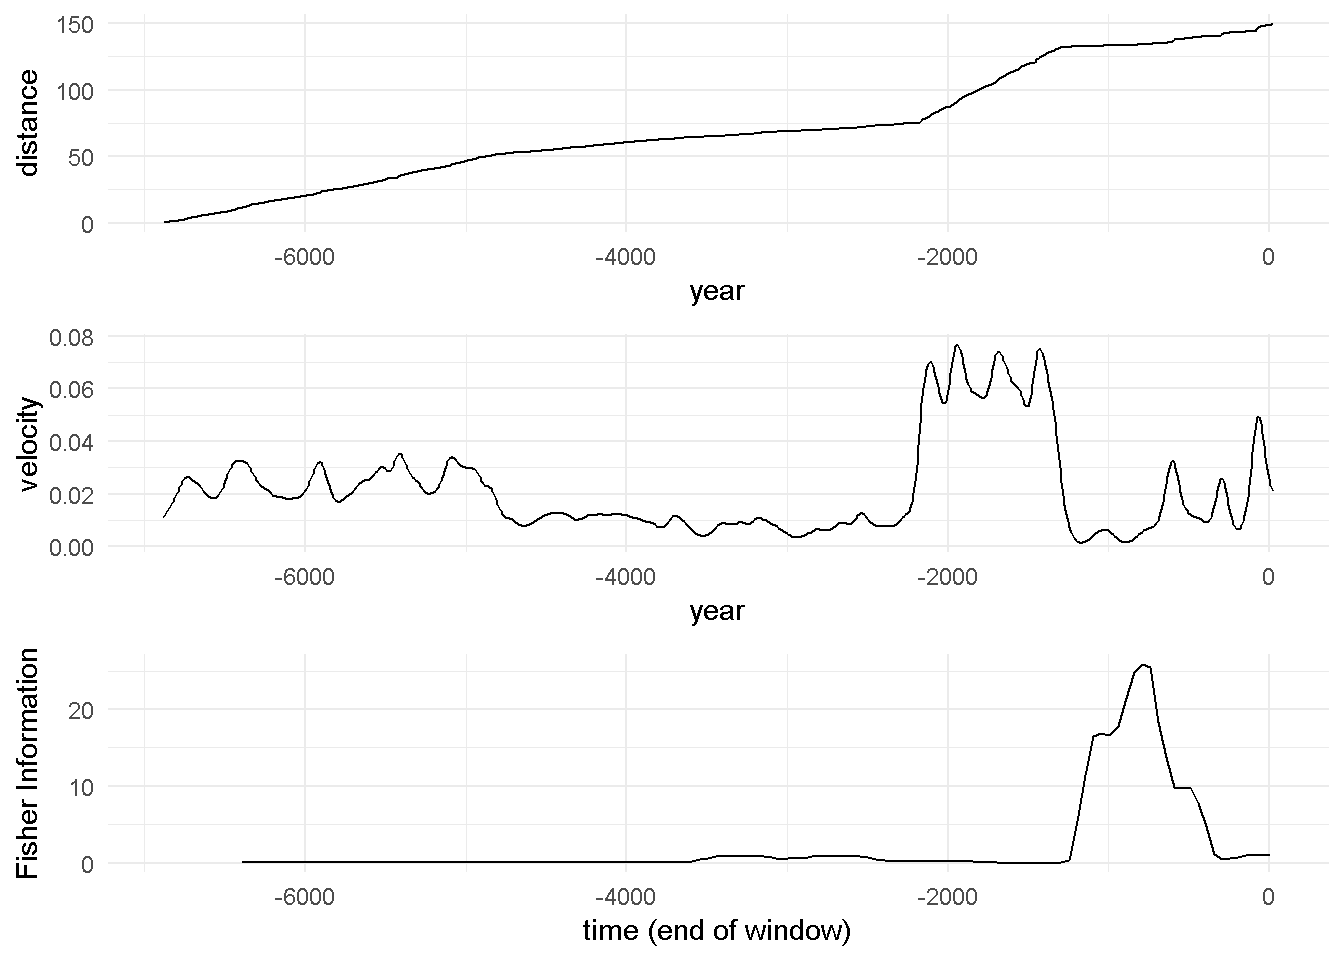
\includegraphics[width=0.95\linewidth]{_myDissertation_files/figure-latex/FIplot-1} \end{center}

\hypertarget{export-figures}{%
\subsection{Export figures}\label{export-figures}}

\hypertarget{bbsRDM}{%
\chapter*{Appendix: R package bbsRDM}\label{bbsRDM}}
\addcontentsline{toc}{chapter}{Appendix: R package bbsRDM}

This appendix contains example analysis associated with the R Package, \texttt{bbsRDM}. Development source code for this package is available on GitHub as a compressed file, \url{https://github.com/TrashBirdEcology/bbsRDM/archive/master.zip} or at \url{https://github.com/TrashBirdEcology/rRDM}.

\hypertarget{regimeDetectionMeasures}{%
\chapter*{Appendix: R package regimeDetectionMeasures}\label{regimeDetectionMeasures}}
\addcontentsline{toc}{chapter}{Appendix: R package regimeDetectionMeasures}

This appendix contains example analysis associated with the R Package, \texttt{regimeDetectionMeasures}. Development source code for this package is available on GitHub as a compressed file at \url{https://github.com/TrashBirdEcology/regimeDetectionMeasures/archive/master.zip} or at \url{https://github.com/TrashBirdEcology/regimeDetectionMeasures}.

\backmatter

\hypertarget{references}{%
\chapter*{References}\label{references}}
\addcontentsline{toc}{chapter}{References}

\markboth{References}{References}

\noindent

\setlength{\parindent}{-0.20in}
\setlength{\leftskip}{0.20in}
\setlength{\parskip}{8pt}

\hypertarget{refs}{}
\leavevmode\hypertarget{ref-abadi2010assessment}{}%
Abadi, F., Gimenez, O., Arlettaz, R., \& Schaub, M. (2010). An assessment of integrated population models: Bias, accuracy, and violation of the assumption of independence. \emph{Ecology}, \emph{91}(1), 7--14.

\leavevmode\hypertarget{ref-andersen_ecological_2009}{}%
Andersen, T., Carstensen, J., Hern??ndez-Garc??a, E., \& Duarte, C. M. (2009). Ecological thresholds and regime shifts: Approaches to identification. \emph{Trends in Ecology \& Evolution}, \emph{24}(1), 49--57. \url{http://doi.org/10.1016/j.tree.2008.07.014}

\leavevmode\hypertarget{ref-angel2000}{}%
Angel, E. (2000). \emph{Interactive computer graphics : A top-down approach with opengl}. Boston, MA: Addison Wesley Longman.

\leavevmode\hypertarget{ref-angel2001}{}%
Angel, E. (2001a). \emph{Batch-file computer graphics : A bottom-up approach with quicktime}. Boston, MA: Wesley Addison Longman.

\leavevmode\hypertarget{ref-angel2002a}{}%
Angel, E. (2001b). \emph{Test second book by angel}. Boston, MA: Wesley Addison Longman.

\leavevmode\hypertarget{ref-beaugrand2004north}{}%
Beaugrand, G. (2004). The north sea regime shift: Evidence, causes, mechanisms and consequences. \emph{Progress in Oceanography}, \emph{60}(2-4), 245--262.

\leavevmode\hypertarget{ref-bestelmeyer_analysis_2011}{}%
Bestelmeyer, B. T., Ellison, A. M., Fraser, W. R., Gorman, K. B., Holbrook, S. J., Laney, C. M., \ldots{} others. (2011). Analysis of abrupt transitions in ecological systems. \emph{Ecosphere}, \emph{2}(12), 1--26.

\leavevmode\hypertarget{ref-boettiger_quantifying_2012}{}%
Boettiger, C., \& Hastings, A. (2012). Quantifying limits to detection of early warning for critical transitions. \emph{Journal of the Royal Society Interface}, \emph{9}, 2527--39.

\leavevmode\hypertarget{ref-boettiger_early_2013}{}%
Boettiger, C., Ross, N., \& Hastings, A. (2013). Early warning signals: The charted and uncharted territories. \emph{Theoretical Ecology}, \emph{6}(3), 255--264.

\leavevmode\hypertarget{ref-brock_variance_2006}{}%
Brock, W., \& Carpenter, S. (2006). Variance as a Leading Indicator of Regime Shift in Ecosystem Services. \emph{Ecology and Society}, \emph{11}(2). \url{http://doi.org/10.5751/ES-01777-110209}

\leavevmode\hypertarget{ref-burthe2016early}{}%
Burthe, S. J., Henrys, P. A., Mackay, E. B., Spears, B. M., Campbell, R., Carvalho, L., \ldots{} others. (2016). Do early warning indicators consistently predict nonlinear change in long-term ecological data? \emph{Journal of Applied Ecology}, \emph{53}(3), 666--676.

\leavevmode\hypertarget{ref-butitta_spatial_2017}{}%
Butitta, V. L., Carpenter, S. R., Loken, L. C., Pace, M. L., \& Stanley, E. H. (2017). Spatial early warning signals in a lake manipulation. \emph{Ecosphere}, \emph{8}(10), n/a--n/a. \url{http://doi.org/10.1002/ecs2.1941}

\leavevmode\hypertarget{ref-byrski2016double}{}%
Byrski, J., \& Byrski, W. (2016). A double window state observer for detection and isolation of abrupt changes in parameters. \emph{International Journal of Applied Mathematics and Computer Science}, \emph{26}(3), 585--602.

\leavevmode\hypertarget{ref-cabezas_towards_2002}{}%
Cabezas, H., \& Fath, B. D. (2002). Towards a theory of sustainable systems. \emph{Fluid Phase Equilibria}, \emph{194}(Supplement C), 3--14. \url{http://doi.org/10.1016/S0378-3812(01)00677-X}

\leavevmode\hypertarget{ref-cabezas_simulated_2005}{}%
Cabezas, H., Pawlowski, C. W., Mayer, A. L., \& Hoagland, N. T. (2005). Simulated experiments with complex sustainable systems: Ecology and technology. \emph{Resources, Conservation and Recycling}, \emph{44}(3), 279--291. Retrieved from \url{http://www.sciencedirect.com/science/article/pii/S092134490500025X}

\leavevmode\hypertarget{ref-chartrand_numerical_2011}{}%
Chartrand, R. (2011). Numerical Differentiation of Noisy, Nonsmooth Data. \emph{International Scholarly Research Notices}. Research article. \url{http://doi.org/10.5402/2011/164564}

\leavevmode\hypertarget{ref-clements2018indicators}{}%
Clements, C. F., \& Ozgul, A. (2018). Indicators of transitions in biological systems. \emph{Ecology Letters}, \emph{21}(6), 905--919.

\leavevmode\hypertarget{ref-dakos_methods_2012}{}%
Dakos, V., Carpenter, S. R., Brock, W. A., Ellison, A. M., Guttal, V., Ives, A. R., \ldots{} Nes, E. H. van. (2012). Methods for detecting early warnings of critical transitions in time series illustrated using simulated ecological data. \emph{PloS One}, \emph{7}(7), e41010.

\leavevmode\hypertarget{ref-dakos_resilience_2015}{}%
Dakos, V., Carpenter, S. R., Nes, E. H. van, \& Scheffer, M. (2015a). Resilience indicators: Prospects and limitations for early warnings of regime shifts. \emph{Philosophical Transactions of the Royal Society B: Biological Sciences}, \emph{370}(1659), 20130263. \url{http://doi.org/10.1098/rstb.2013.0263}

\leavevmode\hypertarget{ref-dakos2015resilience}{}%
Dakos, V., Carpenter, S. R., Nes, E. H. van, \& Scheffer, M. (2015b). Resilience indicators: Prospects and limitations for early warnings of regime shifts. \emph{Philosophical Transactions of the Royal Society B: Biological Sciences}, \emph{370}(1659), 20130263.

\leavevmode\hypertarget{ref-davis_comparing_2008}{}%
Davis, E. P., \& Karim, D. (2008). Comparing early warning systems for banking crises. \emph{Journal of Financial Stability}, \emph{4}(2), 89--120.

\leavevmode\hypertarget{ref-deangelis2017spatially}{}%
DeAngelis, D. L., \& Yurek, S. (2017). Spatially explicit modeling in ecology: A review. \emph{Ecosystems}, \emph{20}(2), 284--300.

\leavevmode\hypertarget{ref-deyoung_regime_2008}{}%
deYoung, B., Barange, M., Beaugrand, G., Harris, R., Perry, R. I., Scheffer, M., \& Werner, F. (2008). Regime shifts in marine ecosystems: Detection, prediction and management. \emph{Trends in Ecology \& Evolution}, \emph{23}(7), 402--409. \url{http://doi.org/10.1016/j.tree.2008.03.008}

\leavevmode\hypertarget{ref-ducre2003comparison}{}%
Ducré-Robitaille, J.-F., Vincent, L. A., \& Boulet, G. (2003). Comparison of techniques for detection of discontinuities in temperature series. \emph{International Journal of Climatology: A Journal of the Royal Meteorological Society}, \emph{23}(9), 1087--1101.

\leavevmode\hypertarget{ref-dutta2018robustness}{}%
Dutta, P. S., Sharma, Y., \& Abbott, K. C. (2018). Robustness of early warning signals for catastrophic and non-catastrophic transitions. \emph{Oikos}, \emph{127}(9), 1251--1263.

\leavevmode\hypertarget{ref-eason_evaluating_2012}{}%
Eason, T., \& Cabezas, H. (2012). Evaluating the sustainability of a regional system using Fisher information in the San Luis Basin, Colorado. \emph{Journal of Environmental Management}, \emph{94}(1), 41--49.

\leavevmode\hypertarget{ref-fath_exergy_2004}{}%
Fath, B. D., \& Cabezas, H. (2004). Exergy and Fisher Information as ecological indices. \emph{Ecological Modelling}, \emph{174}(1), 25--35. \url{http://doi.org/10.1016/j.ecolmodel.2003.12.045}

\leavevmode\hypertarget{ref-fath_regime_2003}{}%
Fath, B. D., Cabezas, H., \& Pawlowski, C. W. (2003). Regime changes in ecological systems: An information theory approach. \emph{Journal of Theoretical Biology}, \emph{222}(4), 517--530. \url{http://doi.org/10.1016/S0022-5193(03)00067-5}

\leavevmode\hypertarget{ref-filatova2016regime}{}%
Filatova, T., Polhill, J. G., \& Ewijk, S. van. (2016). Regime shifts in coupled socio-environmental systems: Review of modelling challenges and approaches. \emph{Environmental Modelling \& Software}, \emph{75}, 333--347.

\leavevmode\hypertarget{ref-fisher_mathematical_1922}{}%
Fisher, R. A. (1922). On the Mathematical Foundations of Theoretical Statistics. \emph{Philosophical Transactions of the Royal Society of London. Series A, Containing Papers of a Mathematical or Physical Character}, \emph{222}, 309--368. Retrieved from \url{http://www.jstor.org/stable/91208}

\leavevmode\hypertarget{ref-frieden_physics_1998}{}%
Frieden, B. R. (1998). \emph{Physics from Fisher information: A unification.} New York, NY: Cambridge University Press.

\leavevmode\hypertarget{ref-frieden_exploratory_2007}{}%
Frieden, B. R., \& Gatenby, R. (Eds.). (2007). \emph{Exploratory Data Analysis Using Fisher Information}. Springer. Retrieved from \url{http://www.springer.com/us/book/9781846285066}

\leavevmode\hypertarget{ref-hastings_regime_2010}{}%
Hastings, A., \& Wysham, D. B. (2010). Regime shifts in ecological systems can occur with no warning. \emph{Ecology Letters}, \emph{13}(4), 464--472. \url{http://doi.org/10.1111/j.1461-0248.2010.01439.x}

\leavevmode\hypertarget{ref-hefley2013statistical}{}%
Hefley, T. J., Tyre, A. J., \& Blankenship, E. E. (2013). Statistical indicators and state--space population models predict extinction in a population of bobwhite quail. \emph{Theoretical Ecology}, \emph{6}(3), 319--331.

\leavevmode\hypertarget{ref-jorgensen_towards_2004}{}%
Jorgensen, S. E., \& Svirezhev, Y. M. (2004). \emph{Towards a Thermodynamic Theory for Ecological Systems}. Elsevier.

\leavevmode\hypertarget{ref-karunanithi_detection_2008}{}%
Karunanithi, A. T., Cabezas, H., Frieden, B. R., \& Pawlowski, C. W. (2008). Detection and assessment of ecosystem regime shifts from fisher information. \emph{Ecology and Society}, \emph{13}(1).

\leavevmode\hypertarget{ref-kefi2014early}{}%
Kefi, S., Guttal, V., Brock, W. A., Carpenter, S. R., Ellison, A. M., Livina, V. N., \ldots{} Dakos, V. (2014). Early warning signals of ecological transitions: Methods for spatial patterns. \emph{PloS One}, \emph{9}(3), e92097.

\leavevmode\hypertarget{ref-kong2017hydrological}{}%
Kong, X., He, Q., Yang, B., He, W., Xu, F., Janssen, A. B., \ldots{} others. (2017). Hydrological regulation drives regime shifts: Evidence from paleolimnology and ecosystem modeling of a large shallow chinese lake. \emph{Global Change Biology}, \emph{23}(2), 737--754.

\leavevmode\hypertarget{ref-litzow_early_2016}{}%
Litzow, M. A., \& Hunsicker, M. E. (2016). Early warning signals, nonlinearity, and signs of hysteresis in real ecosystems. \emph{Ecosphere}, \emph{7}(12), n/a--n/a. \url{http://doi.org/10.1002/ecs2.1614}

\leavevmode\hypertarget{ref-liu_complexity_2007}{}%
Liu, J., Dietz, T., Carpenter, S. R., Alberti, M., Folke, C., Moran, E., \ldots{} others. (2007). Complexity of coupled human and natural systems. \emph{Science}, \emph{317}(5844), 1513--1516.

\leavevmode\hypertarget{ref-liu2013change}{}%
Liu, S., Yamada, M., Collier, N., \& Sugiyama, M. (2013). Change-point detection in time-series data by relative density-ratio estimation. \emph{Neural Networks}, \emph{43}, 72--83.

\leavevmode\hypertarget{ref-mac2014scrutiny}{}%
Mac Nally, R., Albano, C., \& Fleishman, E. (2014). A scrutiny of the evidence for pressure-induced state shifts in estuarine and nearshore ecosystems. \emph{Austral Ecology}, \emph{39}(8), 898--906.

\leavevmode\hypertarget{ref-mantua_methods_2004}{}%
Mantua, N. (2004). Methods for detecting regime shifts in large marine ecosystems: A review with approaches applied to North Pacific data. \emph{Progress in Oceanography}, \emph{60}(2), 165--182. \url{http://doi.org/10.1016/j.pocean.2004.02.016}

\leavevmode\hypertarget{ref-mayer_fisher_2006}{}%
Mayer, A. L., Pawlowski, C. W., \& Cabezas, H. (2006). Fisher Information and dynamic regime changes in ecological systems. \emph{Ecological Modelling}, \emph{195}(1???2), 72--82. \url{http://doi.org/10.1016/j.ecolmodel.2005.11.011}

\leavevmode\hypertarget{ref-mayer_applications_2007}{}%
Mayer, D. A. L., Pawlowski, D. C., Fath, P. B. D., \& Cabezas, D. H. (2007). Applications of Fisher Information to the Management of Sustainable Environmental Systems. In B. R. F. B. MS \& R. A. G. B. MD (Eds.), \emph{Exploratory Data Analysis Using Fisher Information} (pp. 217--244). Springer London. \url{http://doi.org/10.1007/978-1-84628-777-0_7}

\leavevmode\hypertarget{ref-nicholls_detection_2011}{}%
Nicholls, K. H. (2011). Detection of regime shifts in multi-species communities: The Bay of Quinte phytoplankton example. \emph{Methods in Ecology and Evolution}, \emph{2}(4), 416--426. \url{http://doi.org/10.1111/j.2041-210X.2011.00093.x}

\leavevmode\hypertarget{ref-nicholls2011biological}{}%
Nicholls, K., Hoyle, J., Johannsson, O., \& Dermott, R. (2011). A biological regime shift in the bay of quinte ecosystem (lake ontario) associated with the establishment of invasive dreissenid mussels. \emph{Journal of Great Lakes Research}, \emph{37}(2), 310--317.

\leavevmode\hypertarget{ref-perretti2012regime}{}%
Perretti, C. T., \& Munch, S. B. (2012). Regime shift indicators fail under noise levels commonly observed in ecological systems. \emph{Ecological Applications}, \emph{22}(6), 1772--1779.

\leavevmode\hypertarget{ref-perretti_model-free_2013}{}%
Perretti, C. T., Munch, S. B., \& Sugihara, G. (2013). Model-free forecasting outperforms the correct mechanistic model for simulated and experimental data. \emph{Proceedings of the National Academy of Sciences}, \emph{110}(13), 5253--5257.

\leavevmode\hypertarget{ref-petersen2008regime}{}%
Petersen, J. K., Hansen, J. W., Laursen, M. B., Clausen, P., Carstensen, J., \& Conley, D. J. (2008). Regime shift in a coastal marine ecosystem. \emph{Ecological Applications}, \emph{18}(2), 497--510.

\leavevmode\hypertarget{ref-roberts2018early}{}%
Roberts, C. P., Twidwell, D., Burnett, J. L., Donovan, V. M., Wonkka, C. L., Bielski, C. L., \ldots{} others. (2018). Early warnings for state transitions. \emph{Rangeland Ecology \& Management}, \emph{71}(6), 659--670.

\leavevmode\hypertarget{ref-rodionov_brief_2005}{}%
Rodionov, S. N. (2005). A brief overview of the regime shift detection methods. \emph{Large-Scale Disturbances (Regime Shifts) and Recovery in Aquatic Ecosystems: Challenges for Management Toward Sustainability}, 17--24. Retrieved from \url{http://www.beringclimate.noaa.gov/regimes/rodionov_overview.pdf}

\leavevmode\hypertarget{ref-rodionov_application_2005}{}%
Rodionov, S., \& Overland, J. E. (2005). Application of a sequential regime shift detection method to the Bering Sea ecosystem. \emph{ICES Journal of Marine Science}, \emph{62}(3), 328--332. \url{http://doi.org/10.1016/j.icesjms.2005.01.013}

\leavevmode\hypertarget{ref-roy_frieden_physics_1998}{}%
Roy Frieden, B. (1998). \emph{Physics from Fisher information}. Cambridge: Cambridge University Press.

\leavevmode\hypertarget{ref-salehpour2011line}{}%
Salehpour, S., Gustafsson, T., \& Johansson, A. (2011). An on-line method for estimation of piecewise constant parameters in linear regression models. \emph{IFAC Proceedings Volumes}, \emph{44}(1), 3171--3176.

\leavevmode\hypertarget{ref-scheffer_critical_2009}{}%
Scheffer, M. (2009). \emph{Critical transitions in nature and society}. Princeton University Press.

\leavevmode\hypertarget{ref-scheffer_catastrophic_2001}{}%
Scheffer, M., Carpenter, S., Foley, J. A., Folke, C., \& Walker, B. (2001). Catastrophic shifts in ecosystems. \emph{Nature}, \emph{413}(6856), 591--596.

\leavevmode\hypertarget{ref-scheffer2015generic}{}%
Scheffer, M., Carpenter, S. R., Dakos, V., \& Nes, E. H. van. (2015). Generic indicators of ecological resilience: Inferring the chance of a critical transition. \emph{Annual Review of Ecology, Evolution, and Systematics}, \emph{46}, 145--167.

\leavevmode\hypertarget{ref-seddon2014quantitative}{}%
Seddon, A. W., Froyd, C. A., Witkowski, A., \& Willis, K. J. (2014). A quantitative framework for analysis of regime shifts in a galápagos coastal lagoon. \emph{Ecology}, \emph{95}(11), 3046--3055.

\leavevmode\hypertarget{ref-spanbauer_prolonged_2014}{}%
Spanbauer, T. L., Allen, C. R., Angeler, D. G., Eason, T., Fritz, S. C., Garmestani, A. S., \ldots{} Stone, J. R. (2014). Prolonged instability prior to a regime shift. \emph{PLoS One}, \emph{9}(10), e108936.

\leavevmode\hypertarget{ref-steel2013applied}{}%
Steel, E. A., Kennedy, M. C., Cunningham, P. G., \& Stanovick, J. S. (2013). Applied statistics in ecology: Common pitfalls and simple solutions. \emph{Ecosphere}, \emph{4}(9), 1--13.

\leavevmode\hypertarget{ref-sundstrom_detecting_2017}{}%
Sundstrom, S. M., Eason, T., Nelson, R. J., Angeler, D. G., Barichievy, C., Garmestani, A. S., \ldots{} Knutson, M. (2017a). Detecting spatial regimes in ecosystems. \emph{Ecology Letters}, \emph{20}(1), 19--32.

\leavevmode\hypertarget{ref-sundstrom2017detecting}{}%
Sundstrom, S. M., Eason, T., Nelson, R. J., Angeler, D. G., Barichievy, C., Garmestani, A. S., \ldots{} Allen, C. R. (2017b). Detecting spatial regimes in ecosystems. \emph{Ecology Letters}, \emph{20}(1), 19--32. \url{http://doi.org/10.1111/ele.12709}

\leavevmode\hypertarget{ref-vasilakopoulos2017resilience}{}%
Vasilakopoulos, P., Raitsos, D. E., Tzanatos, E., \& Maravelias, C. D. (2017). Resilience and regime shifts in a marine biodiversity hotspot. \emph{Scientific Reports}, \emph{7}(1), 13647.

\leavevmode\hypertarget{ref-walther_ecological_2002}{}%
Walther, G.-R., Post, E., Convey, P., Menzel, A., Parmesan, C., Beebee, T. J., \ldots{} Bairlein, F. (2002). Ecological responses to recent climate change. \emph{Nature}, \emph{416}(6879), 389.

\leavevmode\hypertarget{ref-yin2017methods}{}%
Yin, D., Leroux, S. J., \& He, F. (2017). Methods and models for identifying thresholds of habitat loss. \emph{Ecography}, \emph{40}(1), 131--143.

\leavevmode\hypertarget{ref-zhou2008one}{}%
Zhou, T., \& Shumway, R. (2008). One-step approximations for detecting regime changes in the state space model with application to the influenza data. \emph{Computational Statistics \& Data Analysis}, \emph{52}(5), 2277--2291.


\end{document}
